% TCM: TOTEM Communication Middleware
% Copyright: Copyright (C) 2009-2012
% Contact: denis.conan@telecom-sudparis.eu, michel.simatic@telecom-sudparis.eu
% Permission is granted to copy, distribute and/or modify this document
% under the terms of the GNU Free Documentation License, Version 1.3
% or any later version published by the Free Software Foundation;
% with no Invariant Sections, no Front-Cover Texts, and no Back-Cover Texts.
% A copy of the license is included in the section entitled "GNU
% Free Documentation License".

\documentclass[11pt,a4paper]{article}
\usepackage[T1]{fontenc} % caract�res accentu�s en sortie
\usepackage{lmodern}
\usepackage{geometry} 
\usepackage{graphicx}          % Pour inclure des graphiques
\usepackage{alltt}
\usepackage{listings}
\usepackage{longtable}
\usepackage{url}
\usepackage{multirow} 

\newenvironment{shellcmd}{\begin{small}\begin{alltt}}{\end{alltt}\end{small}}

\geometry{hmargin=2.5cm, vmargin=2.5cm } 
\sloppy % ne pas �tre pointilleux � propos des c�sures de ligne, utiliser
	% plus que l'intervalle normal entre mots si besoin

\newcommand{\num}[1]{\begin{small}\textit{#1}\end{small}}

\usepackage{amssymb}          % Pour inclure des ensembles math�matiques
\RequirePackage[usenames]{color}
\makeatletter
\newcommand{\ygg@basicalert}[2]{\fbox{\bfseries\sffamily\scriptsize#1}{
\sf\small$\blacktriangleright$#2$\blacktriangleleft$}}
\newcommand{\note}[2]{\ygg@basicalert{\textsc{#1}}{\textcolor{red}{#2}}}
\newcommand{\important}[1]{\ygg@basicalert{\textsc{Important}}{\textcolor{red}{#1}}}
\newcommand{\denis}[1]{\ygg@basicalert{\textsc{Denis}}{\textcolor{RedOrange}{#1}}}
\newcommand{\michel}[1]{\ygg@basicalert{\textsc{Michel}}{\textcolor{Purple}{#1}}}
\newcommand{\leif}[1]{\ygg@basicalert{\textsc{Leif}}{\textcolor{RoyalBlue}{#1}}}
\newcommand{\done}[1]{\ygg@basicalert{\textsc{Done}}{\textcolor{OliveGreen}{#1}}}
\newcommand{\donenocomment}{\fbox{\bfseries\sffamily\scriptsize {Done}}{\sf\small}}
\newcommand{\tobedone}[1]{\ygg@basicalert{\textsc{ToBeDone}}{\textcolor{LimeGreen}{#1}}}
\newcommand{\todo}[1]{\ygg@basicalert{\textsc{Todo}}{\textcolor{Mahogany}{#1}}}
\newcommand{\issue}[1]{\ygg@basicalert{\textsc{OpenIssue}}{\textcolor{OrangeRed}{#1}}}
\newcommand{\notsupported}{\fbox{\bfseries\sffamily\scriptsize Not supported}{\sf\small}}
\newcommand{\notsupportedcomment}[1]{\ygg@basicalert{\textsc{NotSupported}}{\textcolor{black}{#1}}}
\newcommand{\postponed}{\fbox{\bfseries\sffamily\scriptsize \textcolor{Sepia}{Postponed}}{\sf\small}}
\newcommand{\irrelevant}[1]{\ygg@basicalert{\textsc{Irrelevant}}{\textcolor{Sepia}{#1}}}
\makeatother

\begin{document}

\title{Presentation of the TOTEM Communication Infrastructure}

\author{Denis Conan, Michel Simatic and Gabriel Adgeg}

\maketitle

\newpage

\begin{center}
\begin{Large}History of changes\end{Large}

~

\begin{longtable}{|l|p{10cm}|}
\hline
\textbf{Date} & \textbf{Changes} \\
\hline
\hline
31st January, 2011 & Initiate with the first version.
\\
\hline
4th February, 2011 & Make it visible to TOTEM partners.\newline
Not finalized to be studied and needs proof reading.\newline 
Contribution is mainly in the appendices.
\\
\hline
18th February, 2011 & New Section~5 ``Example application
demonstrating the integration of the technologies'' (\textsf{Django},
\textsf{RabbitMQ} Broker, \textsf{RabbitMQ} Python Client with
\textsf{Pika}, \textsf{RabbitMQ} Java Client, \textsf{RabbitMQ} Java
Client for Android), game room completed and game play partly
specified.\newline
Move from \textsf{Kombu} to \textsf{Pika}.\\
\hline
21th February, 2011 & Small corrections.\newline
For testing the example application, follow the instructions of
Appendix B (except B.2) and Section 5.3
\\
\hline
25th February, 2011 &  Section~5.2.3 ``Communication architecture
during the game play'' complete.\newline
Code of the example application demonstrating game room and game play
updated.\\
\hline
15th March, 2011 &  First snapshot version of the Java library for
using \textsf{RabbitMQ} in TOTEM in the applications
\textsf{GameMaster}, \textsf{Spectator}, and \textsf{Player}. This API
is to be described in a dedicated section of the document.
\\
\hline
21th March, 2011 &  First snapshot version of the Python library for
using \textsf{RabbitMQ} in TOTEM in the \textsf{GameServer}
(\textsf{GameRoom} server and \textsf{ApplicationInstance}
server). This API is to be described in a dedicated section of the
document.
\\
\hline
23th March, 2011 &  ``Application instance'' is preferred to ``game play''.
\newline
The Section~A of the appendix describing EBS, AMQP and
\textsf{RabbitMQ} is completed.
\\
\hline
28th March, 2011 &  New Section on the ``API of the communication
infrastructure'', that is on the user manual of the communication
infrastructure using \textsf{RabbitMQ}.
\newline
Java Android TOTEM library decomposed into four modules:
\textsf{common}, \textsf{game\-master\-application},
\textsf{player\-application}, and \textsf{spectator\-application}.
\\
\hline
29th March, 2011 & New Section on the ``Requirements'', with for
each of them some comments and the status.
\newline
Add status of sections in the introduction.
\newline
First draft of the Section~\ref{S_use_case} introducing the illustrative
application. The content was previously in the analysis subsection of
Section~\ref{S_integration}.
\newline
First draft of the Section~\ref{S_presentation_concepts} introducing
the AMQP concepts. The content was previously in the appendix.
\newline
Example integration application with Java Android Clients,
\textsf{Game Master}, \textsf{Player}, and \textsf{Spectator}.
\\
\hline
30th of March, 2011 &
Add a figure of AMQP concepts in Section~\ref{S_presentation_concepts}.
\newline
First draft of the system architecture with a focus in communication
infrastructure in Section~\ref{S_architecture}.
\newline
First draft of the detailed design, with figures moved from
Section~\ref{S_integration} to Section~\ref{S_detailed_design}.
\\
\hline
15th of April, 2011 &
Moving RabbitMQ server from version 2.3.1 to version 2.4.1.
\newline
Reorganize Section~\ref{S_installation_rabbitmq_local} and add a
subsection on a JavaScript client example.
\\
\hline
30th of April, 2011 &
The Section ``Requirements'' has been updated to current status.
\newline
The game room server using \textsf{RabbitMQ} is replaced by a game
server using \textsf{XML-RPC} to control the game instances, which use
\textsf{RabbitMQ}. The term ``application instance server'' is
replaced by ``game logic server'' and the code is separated from the
game server.
\newline
The API is complemented with methods to publish to all and to a
consumer.
\newline
New section ``Organisation of the source code'' to describe the
directory structure of the Subversion Repository.
\\
\hline
2nd of May, 2011 &
Update of the Section ``Example application demonstrating the integration of the technologies''.
\newline
Android clients updated to the last version of the example application.
\\
\hline
9th of May, 2011 &
Add instructions in Section ``Installation of RabbitMQ'', for installing and checking the version number of Erlang, SunJDK, Maven, and Python.
\newline
Add instructions in Section ``Installation of RabbitMQ'' for w-getting \textsf{RabbitMQ}.
\newline
Add a new Section ``Short tutorial on how to design and implement a
new protocol''.
\newline
The example application does no more use \textsf{Django}, the
integration to the \textsf{Django} game server is done elsewhere. Any
previously existing \textsf{Django} parts are removed.
\\
\hline
11th of May, 2011 &
Defensive programming of the Java TOTEM Communication Library: the
semantics of the publications is ``at least once'', thus the Section
``Detailed design of the communication infrastructure'' is updated
with this new design decision.
\newline
New script for the automatic running of the example application with
Android Emulators.
\\
\hline
26th of May, 2011 &
In order to prepare the integration with the MPEG4 Player, the TOTEM
library is complemented with a TOTEM RabbitMQ Proxy on Android.
\\
\hline
8th of July, 2011 &
Appendix updated with version 2.5.1 of RabbitMQ. New Author Gabriel Adgeg.
\\
\hline
2nd of August, 2011 &
New appendix for RabbitMQ client in Javascript with node.js. Former Javascript appendix is not removed, since it should be used with clients that cannot use node.js.
\\
\hline
9th of August, 2011 &
Corrections added to the appendix for RabbitMQ client in Javascript with node.js. Useless diagram removed. Output of the execution of the Step1 added.
\\
\hline
22nd of August, 2011 &
New project in directory \texttt{RabbitMQ/Tests/proxy-node-amqp}. A
proxy implemented with \textsf{Node.js} is provided to communicate
with the \textsf{RabbitMQ} broker. A web client is also provided to
communicate with the proxy in order to receive messages from a given
queue. All the details to install and launch this example are located
in the file \texttt{readme.txt}. 
\\
\hline
27th of September, 2011 &
New version of Android Java client applications of the integration example application.
\\
\hline
17th of October, 2011 &
Move to version 2.5.1 of RabbitMQ.
\newline
Deprecated appendix for RabbitMQ Javascript plugin removed.
\newline
Appendix for Java J2SE clients is set to deprecated since these
have not been updated to the latest version of TOTEM library.
\newline
Description of Javascript subsystems for Master and Spectator
applications running in a browser added.
\newline
Installation procedure of XMLRPC library for Node.js added.
\\
\hline
18th of October, 2011 &
Appendix for installing \textsf{RabbitMQ} on Amazon EC2 stated to
status deprecated since the section has not already been updated to
the last version.
\newline
Appendix for adapting \textsf{RabbitMQ} Java client library to Android
phones removed since the adaptation is not needed anymore.
\\ 
\hline
25th of October, 2011 &
Implementation and execution note updated with new Javascript configuration 
files. 
\newline
Node.js installation procedure corrected.
\newline
References to RabbitMQ proxy for MPEG player removed.
\\
\hline
9th of November, 2011 &
New figures to present the architecture of the middleware.
\newline
Notes added on parts that will be updated soon.
\newline
Organisation of the source code updated.
\\
\hline
7th of December, 2011 &
Python source code modified to fix the pika.NotImplementedError bug.
\\
\hline
15th of December, 2011 &
Full support of several parallel game instances.
\newline
New XMLRPC methods to list game instances or to terminate a single game instance.
\newline
RabbitMQ-Totem library in JavaScript: state machine, action kind, actions, transparent consumption of messages.
\newline
Possibility to host several Masters and Spectators JavaScript applications of different games on a single NodeJs proxy.
\newline
Python projects for GameServer and GameLogicServer changed in PyDev projects.
\\
\hline
22th of December, 2011 &
Performances of the middlaware are added to the 
requirements section.
\\
\hline
18th of January, 2012 &
Installation of NPM updated, since curl command is required.
\newline
Version 0.1.0 of AMQP library for Node is required, since bugs seem to appear in later versions. 
\\
\hline
6th of February, 2012 &
References to Logging server changed in Chapter 2.
\newline
Requirements updated with precisions about the presence service and HTTP 
communication.
\newline
Short presentation of Node.js, and of its choice in Chapter 4.
\newline
Design decisions concerning AMQP ressources added in Chapter 6. 
\\
\hline
6th of February, 2012 &
Presentation of AMQP concepts for JavaScript in Chapter 6.
\newline
New XML-RPC methods added in the Figure of the architecture-game-server.
\newline
JavaScript idioms added to Chapter 7.
\newline
JavaScript API directory is added to Chapter 8.
\newline
Tutorial replaced with the one used during the Lab. Some explanations have
been modified for a better understanding. 
\\
\hline
15th of February, 2012 &
Presentation of the concepts of the middleware(the use of XML-RPC, actions and 
actions kinds...)  added to the tutorial Section.
\newline
Many details added to the tutorial to detail the points where students had 
problems during the Lab.
\newline
New tutorial for the JavaScript applications. 
\newline
Methods refactored with new version of API in the tutorial.
\newline
Section "Integration of technologies" updated to new contents on the SVN
\newline
Obsolete appendix for Android phones removed.
\newline
Appendix for J2SE applications corrected.
\newline
Version of the RabbitMQ broker is set to 2.7.1.
\\
\hline
\end{longtable}
\end{center}

\newpage

\tableofcontents

\newpage

\section*{License of TOTEM communication middleware}

\begin{verbatim}
TCM: TOTEM Communication Middleware
Copyright: Copyright (C) 2009-2012
Contact: denis.conan@telecom-sudparis.eu, michel.simatic@telecom-sudparis.eu

This library is free software; you can redistribute it and/or
modify it under the terms of the GNU Lesser General Public
License as published by the Free Software Foundation; either
version 3 of the License, or any later version.

This library is distributed in the hope that it will be useful,
but WITHOUT ANY WARRANTY; without even the implied warranty of
MERCHANTABILITY or FITNESS FOR A PARTICULAR PURPOSE. See the GNU
Lesser General Public License for more details.

You should have received a copy of the GNU Lesser General Public
License along with this library; if not, write to the Free Software
Foundation, Inc., 59 Temple Place, Suite 330, Boston, MA  02111-1307
USA

Developer(s): Denis Conan, Gabriel Adgeg
\end{verbatim}

\newpage

\section{Introduction}
\label{S_introduction}

\noindent NB: This document is a living document.

\bigskip

\noindent Status of the sections of the document:
\begin{itemize}
\item Section~\ref{S_introduction}, ``Introduction'': Complete.
\item Section~\ref{S_use_case}, ``Illustrative scenarios and use
  cases'': Complete.
\item Section~\ref{S_requirements}, ``Requirements for the
  communication infrastructure'': Complete.
\item Section~\ref{S_presentation_concepts}, ``Presentation of EBS,
  AMQP, RabbitMQ and Node.js'': Complete.
\item Section~\ref{S_architecture}, ``Architecture of the
  communication infrastructure'': Complete.
\item Section~\ref{S_detailed_design}, ``Detailed design of the
  communication infrastructure'': Complete.
\item Section~\ref{S_api}, ``API of the communication infrastructure'': Complete.
\item Section~\ref{S_sourcecode}, ``Organisation of the source code'':
  Complete. 
\item Section~\ref{S_tutorialprotocol}, ``Tutorial on how to
  design and implement a new protocol'': Complete.
\item Section~\ref{S_integration}, ``Example application demonstrating
  the integration of the technologies'': Complete.
\item Section~\ref{S_installation_rabbitmq_local}, ``Installation of
  RabbitMQ'': Complete.
\item Section~\ref{S_installation_rabbitmq_ec2}, ``Installation of
  RabbitMQ and Pika on Amazon EC2'': Complete but deprecated.
\end{itemize}

\newpage
% TCM: TOTEM Communication Middleware
% Copyright: Copyright (C) 2009-2012
% Contact: denis.conan@telecom-sudparis.eu, michel.simatic@telecom-sudparis.eu
% Permission is granted to copy, distribute and/or modify this document
% under the terms of the GNU Free Documentation License, Version 1.3
% or any later version published by the Free Software Foundation;
% with no Invariant Sections, no Front-Cover Texts, and no Back-Cover Texts.
% A copy of the license is included in the section entitled "GNU
% Free Documentation License".

\section{Illustrative scenarios and use cases}
\label{S_use_case}

In this section, and through the document, we illustrate the TOTEM
communication infrastructure with an illustrative application
demonstrating the integration of many of the TOTEM technologies. The
objective of this example application is to help in eliciting the
requirements of the communication infrastructure in
Section~\ref{S_requirements}. The subsystems and the actors are
modelled in the UML use case diagrams of Figures~\ref{F_use_case_login}
and~\ref{F_use_case}. Since this document describes the communication
infrastructure, we decided to present two different diagrams to better
state where and when the two technologies \textsf{XML-RPC} and
\textsf{RabbitMQ} are involved: Figure~\ref{F_use_case_login} shows
the subsystems at the beginning of the application when the end-users
log in using the \textsf{XML-RPC} communication technology;
Figure~\ref{F_use_case} shows the subsystems during the game play of a
game instance when the communication exchanges are performed using the
\textsf{RabbitMQ} technology \footnote{For the sake of simplicity, we
  have ignored the termination of the application bringing another
  subsystem into play, which calls the \textsf{Game Server} for
  organising the termination of all the subsystems using
  \textsf{AMQP} messages.}:

\begin{itemize}
\item The actors of the use case diagrams of
  Figures~\ref{F_use_case_login} and~\ref{F_use_case} are the
  participants of the example application and the systems are the
  subsystems. In Figure~\ref{F_use_case}, since the \textsf{Game
    Broker} is  not a ``functional''
  but a ``technical'' subsystem, it is not present in the use case
  diagram. Please observe also that we do not restrict ourselves and
  allow for direct point to point communication between the
  \textsf{Master Application}, the \textsf{Player Application} and the
  \textsf{Spectator System}, without the intermediary of the
  \textsf{Game Server}. All the relevant events are logged by the 
  \textsf{Logging Server}, for instance for post-mortem debugging. It
  provides logging functionalities to all the other subsystems (this
  is modelled in Figure~\ref{F_use_case} by the many arrows pointing
  to the LoggingServer). 
\item End-user subsystems connect to the \textsf{Game Server} and log
  in. Game instances are created by the \textsf{Game Server}. For the
  sake of simplicity, we consider only one game server managing all
  the games and all the game instances. In this document, we consider
  only one game instance. A game instance is managed by a
  \textsf{Game Logic Server}, which is the server that
  contains all the game logic of the game for that instance.
\item The \textsf{Master Application} is the application used by the
  game master to create and manage a new game instance. For the sake
  of simplicity, we only assign a name to a game and a name to a game
  instance. In the example application, game masters do not intervene
  to accept or refuse the joining of players or spectators.
\item The \textsf{Player Application} corresponds to the game
  application executed by the game player. In this simplistic example,
  a player application can only join or leave a game instance, and
  exchange notifications to and from the game server or the other game
  entities (master, players, spectators).
\item The \textsf{Spectator System} is used by non-players to be
  informed about events of the game instance. Spectators register to
  categories of events. The events sent to the spectators do not need
  to pass through the \textsf{Game Logic Server}
\end{itemize}

\begin{figure}[htbp!]
\begin{center}
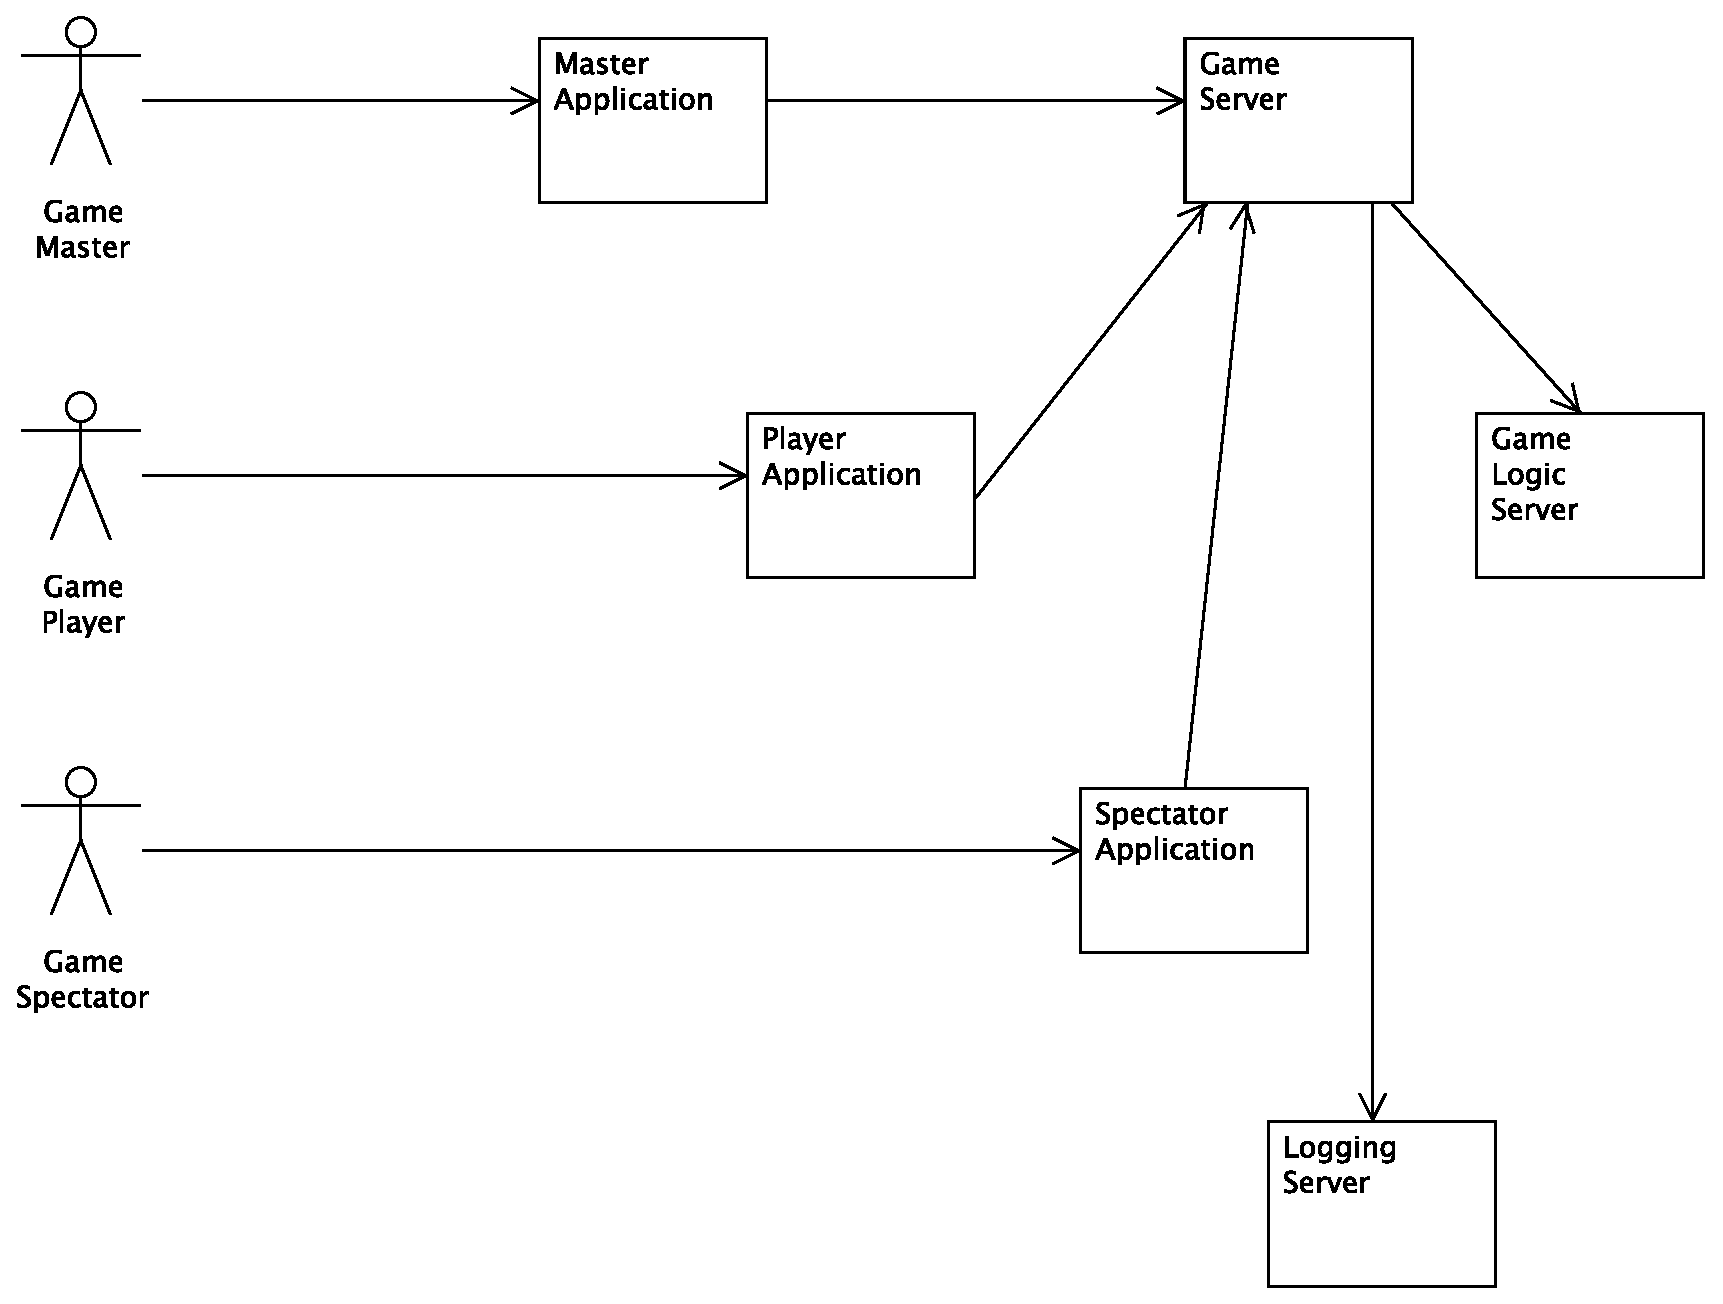
\includegraphics[scale=0.6]{Figures/_use_case_login}
\caption{Illustrative use case ---when log in using \textsf{XML-RPC}}
\label{F_use_case_login}
\end{center}
\end{figure}

\begin{figure}[htbp!]
\begin{center}
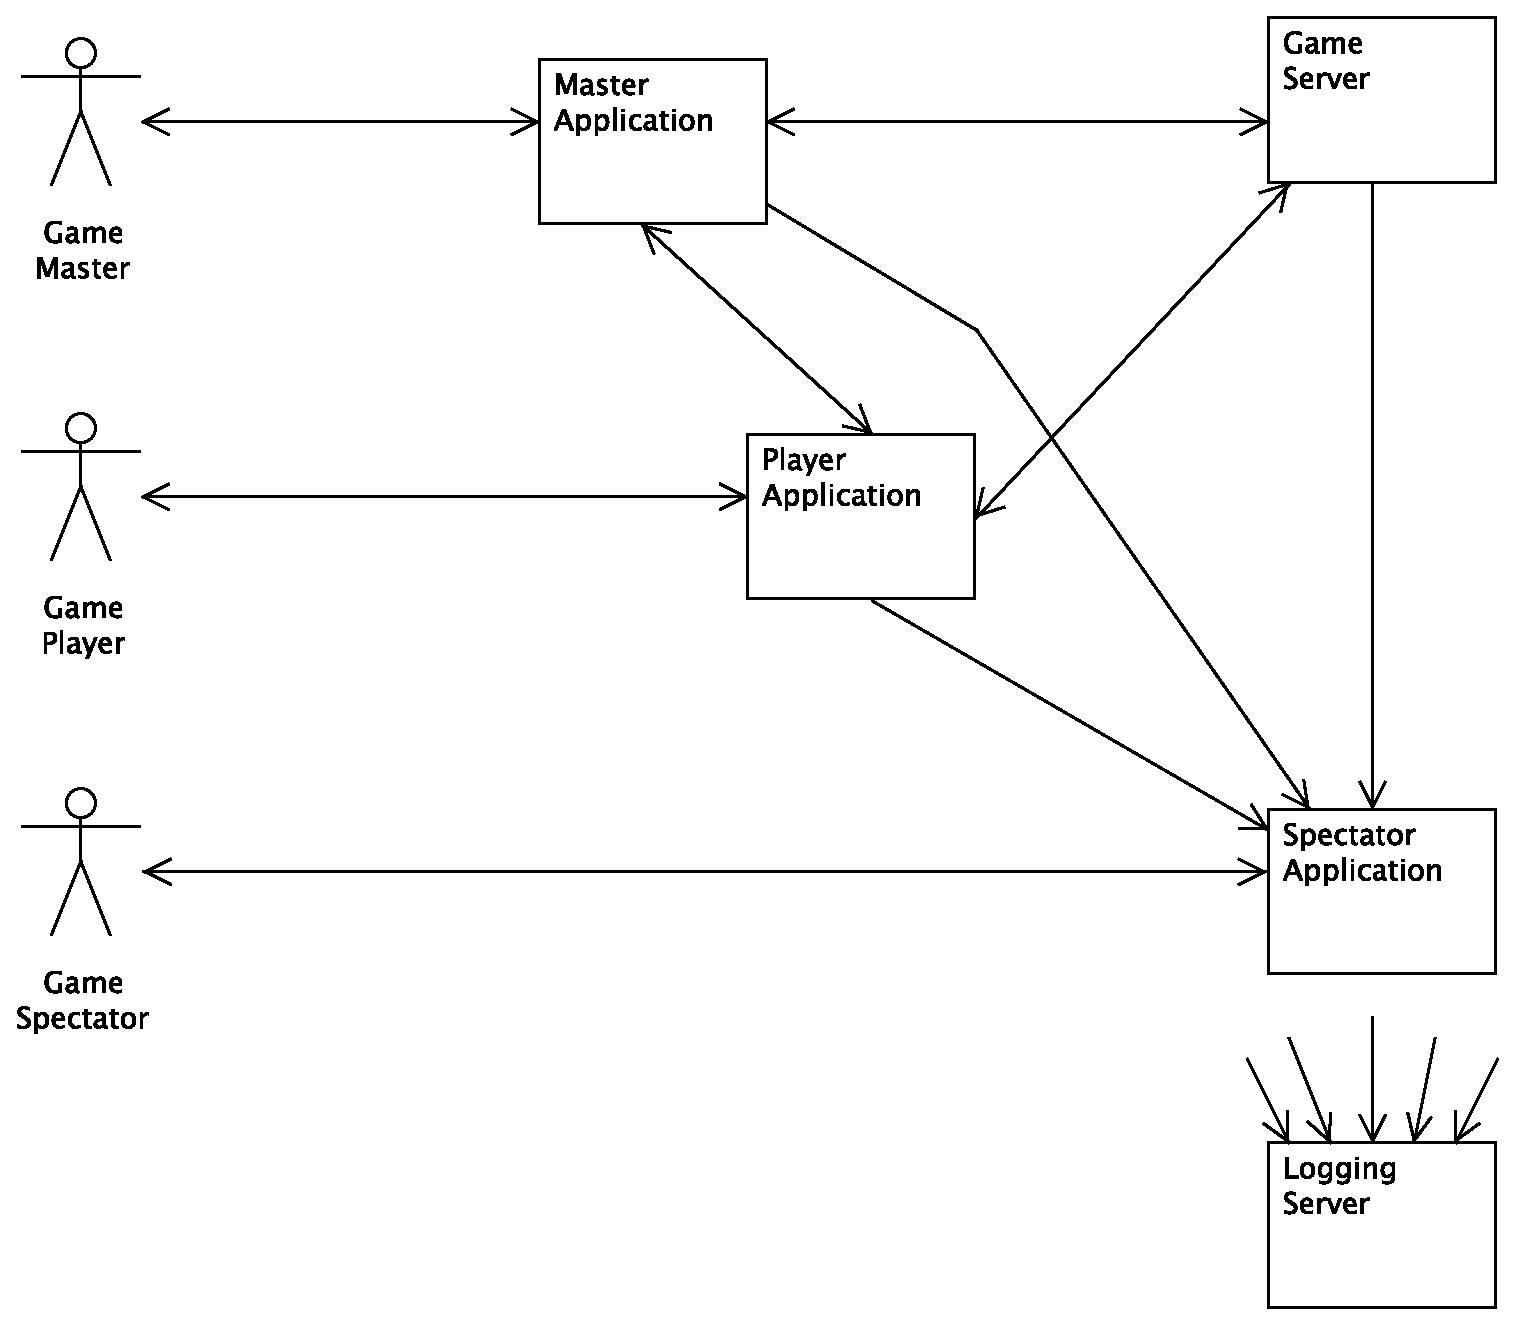
\includegraphics[scale=0.6]{Figures/_use_case}
\caption{Illustrative use case ---during the game play using\textsf{RabbitMQ}}
\label{F_use_case}
\end{center}
\end{figure}

% actors
% dessin use case avec la plate-forme TOTEM comme une bo�te noire et les acteurs
% - game platform admin
%   - Django
%   - RabbitMQ
% - game master
% - player
% - spectator

% illustrative scenario
% dessins activit�s du d�marrage d'un jeu
% - sc�nario de l'application exemple +
%   figure 4 (Activity diagram of the creation of the game and the
%             game instance, and of the joining of players and spectators)
%   - 1 couleur par acteur
%   - �v�nements, actions
%     - terminologie pour admin sys Django et RabbitMQ

\newpage
% TCM: TOTEM Communication Middleware
% Copyright: Copyright (C) 2009-2012
% Contact: denis.conan@telecom-sudparis.eu, michel.simatic@telecom-sudparis.eu
% Permission is granted to copy, distribute and/or modify this document
% under the terms of the GNU Free Documentation License, Version 1.3
% or any later version published by the Free Software Foundation;
% with no Invariant Sections, no Front-Cover Texts, and no Back-Cover Texts.
% A copy of the license is included in the section entitled "GNU
% Free Documentation License".

\section{Requirements for the communication infrastructure}
\label{S_requirements}

The requirements listed in this section are the
requirements for the communication infrastructure with their corresponding 
status.

\begin{enumerate}
\item Messaging
\label{R_1}
\begin{enumerate}
\item Destination of message
\label{R_1_a}
\begin{enumerate}
\item Point-to-point: From one entity (game server, game master, gamer
  / player, or spectator) to any other entity which the sending entity
  is aware of. (Mandatory)
\label{R_1_a_i}
\begin{itemize}
\item \done{All the bindings (between exchanges and queues) and
  the routing keys of the messages include the identity of the sender
  and of the addressee or ``all'' (all the entities).}
\end{itemize}
\item Broadcast to game players: It is possible for one entity (game
  server, game master, gamer / player, or spectator) to broadcast to
  all the other entities (including itself) (Mandatory)
\label{R_1_a_ii}
\begin{itemize}
\item \done{Using ``all'' as the addressee in the routing key, a
  message is broadcast to all the entities of the game instance. Note
  that the sender also receives its broadcast message.}
\end{itemize}
\end{enumerate}
\item Type of messages
\label{R_1_b}
\begin{enumerate}
\item Notification: An entity is able to send (``fire and forget''
  mode) an information to other entity(ies). (Mandatory)
\label{R_1_b_i}
\begin{itemize}
\item \done{This is the messaging paradigm of AMQP\footnote{The
    middleware \textsf{RabbitMQ} used for communication during the
    game play conforms to the standard AMQP, Advanced Message Queuing
    Protocol. Both AMQP and \textsf{RabbitMQ} are introduced in
    Section~\ref{S_presentation_concepts}.}.}
\end{itemize}
\item Request/Response: When an entity sends such a message, it blocks
  itself until it receives a response to its request (RPC
  mode). (Mandatory)
\begin{itemize}
\item \done{This is the messaging paradigm of XML-RPC. The login
  exchanges are performed using RPC mode.}
\end{itemize}
\label{R_1_b_ii}
\item Request/Response with ``future'': When an entity sends such a
  message, it continues operation and receives a delivery receipt at a
  later stage. (Important)
\begin{itemize}
\item \done{Futures can be implemented during the game play. This feature is 
not demonstrated in the illustrative application. But ask for
  an example to communication infrastructure designers when needed.}
\end{itemize}
\label{R_1_b_iii}
\end{enumerate}
\item Message reliability: Each message has a ``reliability''
  attribute. (Important)
\label{R_1_c}
\begin{itemize}
\item If this attribute is set to true, message will arrive to all of
  its destinations (even in the case of a broadcast message), even
  though some mobiles crashed or are disconnected.  However, if a
  mobile crashes and recovers, or disconnects for more than a given
  number of minutes (this number is configured at game server level),
  messages will be lost (this is to prevent the broker and the mobiles
  from being overflowed by undelivered messages).
\begin{itemize}
\item \done{This corresponds to the ``persistent'' attribute of
  messages in AMQP specification. By default, messages are not
  persistent. This feature is not demonstrated in the illustrative application.
  But ask for an example to communication infrastructure
  designers when needed. In addition, AMQP queues can be durable, that
  is they survive a broker crash and restart.}
\end{itemize}
\item If this attribute is set to false, messages can be lost.
\begin{itemize}
\item \done{This is the default configuration of AMQP messages.}
\end{itemize}
\end{itemize}
\item Order of messages
\label{R_1_d}
\begin{enumerate}
\item FIFO: Messages originating from the same source are received in
  the order with which they were sent by all the recipients. (Mandatory)
\label{R_1_d_i}
\begin{itemize}
\item \done{\textsf{RabbitMQ} guarantees ordering of the messages, as
  long as the messages in question follow the exact same path through
  the clients and the broker (same publisher, same exchange, same
  queue and same consumer). Be careful! This remains true as long as
  the broker does not crash and recover.}
\end{itemize}
\end{enumerate}
\item Platform-independent message encoding: The communication
  middleware is able to take care of problems related to differences
  of data encoding on the different platforms participating to the
  communication (Endian problem, Strings encoding...). (Important)
\label{R_1_e}
\begin{itemize}
\item \done{\textsf{Rabbit} treats a message payload as an opaque
  binary. We use Strings coding.}
\end{itemize}
\item Message security: Messages can be
  encrypted in order to avoid the decoding of messages contents by
  third parties. (Nice to have)
\label{R_1_f}
\begin{itemize}
\item \issue{AMQP promotes the use of SASL, which hasn't been experimented yet.}
\end{itemize}
\end{enumerate}
\item Presence service: At any time, an entity (mobile or game server)
  knows which session members are accessible.
\label{R_2}
\begin{itemize}
\item \postponed
\end{itemize}
\item Disconnection management (Mandatory, risk Medium). In case of
  disconnection (triggered by the application or not) from the broker,
  a mobile (Reminder: we assume that the game server is always
  connected to the broker) must:
\label{R_3}
\begin{enumerate}
\item Be aware of disconnection from network
\label{R_3_a}
\begin{itemize}
\item \done{Libraries developed for Java J2SE, Android and JavaScript 
applications have a ``maximum number of retries'' property, which can be set by
the user. If a disconnection occurs during the consumption or the publication 
of messages, 
the library tries to reconnect, to consume and possibly to publish messages 
(every second) until the maximum number of retries value is reached. If the 
network stays 
unreachable after this time period, the application stops its reconnection 
routine and the messages intended to this application stay on the broker 
queues.}
\end{itemize}
\item Be aware of the disconnection from the broker
\label{R_3_b}
\begin{itemize}
\item \postponed
\end{itemize}
\item Have tools to go on communicating:
\label{R_3_c}
\begin{enumerate}
\item The communication middleware always accepts messages from the
  application which uses it, even if it cannot communicate with the
  other entities (e.g. other mobiles and server) participating to the
  protocol.

  Said in other words: Messages are queued locally on the mobile
  rather than being deleted because the mobile is not connected to the
  broker. When connection to the broker is back, these queued messages are
  sent.
\label{R_3_c_i}
\begin{itemize}
\item \postponed
\end{itemize}
\item Each message can be given a delivery timeout. If such a timeout
  is set and the message is not delivered to destination after such
  timeout, an exception is sent to the application. The application
  can invoke a primitive to cancel such a message.
\label{R_3_c_ii}
\begin{itemize}
\item \postponed
\end{itemize}
\end{enumerate}
\end{enumerate}
\item Can send small messages as well as large binary blobs (e.g. from
  Location Survey tool). (Important)
\label{R_4}
\begin{itemize}
\item \done{By introducing the concept of framing, AMQP messages are
  chopped up into frames for interleaving on transport, which is
  useful for instance for large messages.}
\end{itemize}
% Functionalities developed by Totem project on top of the
% communication middleware to facilitate multiplayer game development
\item Totem offers game session concept above the communication
  middleware. In particular, broadcasts are sent to all session
  members. (Important)
\label{R_5}
\begin{itemize}
\item \done{This is the role of this document to introduce for such
  concept of game session through the AMQP concepts of virtual host,
  exchange, queue, routing key and binding.}
\end{itemize}
% Access to all of the functionalities (provided by the communication
% middleware and developed on top of it) by an application
\item Integrates with web framework
\label{R_8}
\begin{enumerate}
\item The web framework is able to send/receive messages through/from
  the communication middleware. (Mandatory)
\label{R_6_a}
\begin{itemize}
\item \donenocomment
\end{itemize}
\item The code of the broker can be integrated within the code of the
  framework. (Nice to have)
\label{R_6_b}
\begin{itemize}
\item \donenocomment
\end{itemize}
\end{enumerate}
\item An (Android) mobile client is able to send/receive messages
  through/from the communication middleware. (Mandatory)
\label{R_7}
\begin{itemize}
\item \done{The integration of Android running mobile devices is
  demonstrated in the example application of
  Section~\ref{S_integration}.}
\end{itemize}
\item A client (mobile or server) can communicate with the
  communication middleware through HTTP protocol. This protocol is
  used to connect the MPEG player and the communication
  middleware. This protocol may also be used in the case Telecom
  operators do not allow direct socket connections from mobile to the
  Internet. In this case, the mobile has to use HTTP protocol instead
  of plain socket-based library. (Mandatory)
\label{R_8}
\begin{itemize}
\item \done{Libraries are provided to enable communication between JavaScript 
applications and the broker (through a proxy). The communication is made with 
HTTP via AJAX requests.}
\end{itemize}
\item Easy setup and deployment. (Mandatory)
\label{R_9}
\begin{itemize}
\item \done{This document includes several sections in the appendix
  describing installation procedures.}
\end{itemize}
\item Standards based (Important).
\label{R_10}
\begin{itemize}
\item \done{\textsf{RabbitMQ} conforms to the version 0.9.1 of AMQP
  standard.}
\end{itemize}
\item Broker is able to push messages to game server (Mandatory, risk
  zero)
\label{R_11}
\begin{itemize}
\item \done{AMQP protocol pushes messages as soon as the consumer asks
  for it. By dedicating a thread for consuming messages in a loop,
  messages will be pushed by the broker at the speed of consumer
  calls of the AMQP command \texttt{consume}.}
\end{itemize}
\item Broker is able to push messages to mobiles (Important as it
  lowers latency for delivering messages to mobiles. Nevertheless it
  is not mandatory, as game design can limit the visibility of an
  important latency.)
\label{R_12}
\begin{itemize}
\item \done{Same answer as for Requirement~\ref{R_11}.}
\end{itemize}
\item On the mobile, if multiple communication channels (Wifi, GPRS,
  etc.) are available
\label{R_13}
\begin{enumerate}
\item When the player launches a game, the game tries to connect
  to the broker: We rely on the mobile OS to choose (or give to the
  user the choice of) the communication channel to use to connect to
  the broker (Mandatory, risk Medium: On Android, we can use method
  setNetworkPreference of the ConnectivityManager but there is little
  documentation).
\label{R_13_a}
\begin{itemize}
\item \irrelevant{Not an issue for the communication middleware.}
\end{itemize}
\item In the case the mobile was connected to Wifi and the player gets
  out of the Wifi zone, the telephone reconnects automatically to
  another available network (Nice to have because the player is not
  aware that it is going to use her data plan now).
\label{R_13_b}
\begin{itemize}
\item \irrelevant{Not an issue for the communication middleware.}
\end{itemize}
\item We keep track of ``free'' Internet connections of the user
\label{R_13_c}
\begin{itemize}
\item \irrelevant{Not an issue for the communication middleware.}
\end{itemize}
\end{enumerate}
\item Integrates with Android Cloud to Device Messaging Framework
  (Nice to have, as it is Android specific.)
\label{R_14}
\begin{itemize}
\item \irrelevant{It is a feature which allows to send small out of
  application messages. It does not have to be integrated with
  \textsf{RabbitMQ}.}
\end{itemize}
% Performance
\item Latency. Communication middleware requires a maximum of 100
  milliseconds (100 is an estimation which should fit most of Totem
  games) to send a message from a mobile client to the game server (if
  the mobile is connected with the broker thanks to a Wifi network).
\label{R_15}
\begin{itemize}
\item \done{
In the following array, we present the average performances for the publication 
and the consumption of one message containing about 10 characters. 
Results are given in milliseconds. 
\begin{tabular}{|l|l|c|c|} \hline
Client & Network & Publish & Consume  \\ \hline
\multirow{2}{*}{Android application} & WiFi & 2.9 & 7.8 \\
& 3G+ & 1.6 & 120 \\ \hline
\multirow{2}{*}{JavaScript application} & WiFi & 10.9 & 111 \\
& 3G+ & 18.2 & 371 \\ \hline
\end{tabular}
\label{mw_performances}}

\end{itemize}
\item Throughput. Communication middleware is able to withstand at
  least 1 notification per mobile client per second per game server
  (the configuration of each game server is the configuration of a
  free Amazon server), with at least 500 mobile clients. Above 500
  clients (this 500 number is currently an estimation; A more precise
  value should be computed thanks to a marketing study!), we consider
  that the game editor has enough customers to be able to pay for the
  Cloud service.
\label{R_16}
\begin{itemize}
\item \issue{Confident, but not experimented because no performance
  tests, yet.}
\end{itemize}
% Miscellaneous
\item Identity, user management (ideally via Facebook Connect, OAuth,
  OpenID, etc.) (Mandatory). If the communication
  middleware requires user login functionality, this functionality
  database can be replaced by mechanisms like Facebook Connect, OAuth,
  OpenID, etc.
\label{R_17}
\begin{itemize}
\item \irrelevant{The TOTEM \textsf{Django} game server manages the
  log-ins and passwords. Thus, it is not an issue for the
  communication middleware.}
\end{itemize}
\item Cloud support: Amazon, or Google App Engine. (Mandatory)
\label{R_18}
\begin{itemize}
\item \done{The cloud integration is not demonstrated with Google
  App. Engine (since the latter provides its own software
  infrastructure), but with Amazon
  EC2. Cf.~Section~\ref{S_installation_rabbitmq_ec2} of the appendix
  for the installation procedure.}
\end{itemize}
\end{enumerate}

\endinput

\newpage
% TCM: TOTEM Communication Middleware
% Copyright: Copyright (C) 2009-2012
% Contact: denis.conan@telecom-sudparis.eu, michel.simatic@telecom-sudparis.eu
% Permission is granted to copy, distribute and/or modify this document
% under the terms of the GNU Free Documentation License, Version 1.3
% or any later version published by the Free Software Foundation;
% with no Invariant Sections, no Front-Cover Texts, and no Back-Cover Texts.
% A copy of the license is included in the section entitled "GNU
% Free Documentation License".

\section{Presentation of EBS, AMQP, \textsf{RabbitMQ} and \textsf{Node.js}}
\label{S_presentation_concepts}

This section presents the communication infrastructure concepts of the
AMQP specification and the middleware \textsf{RabbitMQ} used for
event-based notification in the TOTEM project. The other communication
paradigm used in the TOTEM project is RPC, more precisely by
bringing into play the XML-RPC standard. Since TOTEM partners are more
used with XML-RPC, we only present AMQP.

\subsection{Presentation of Event-Based Systems}
\label{SS_presentation_ebs}

In this section, we briefly introduce the basic concepts and
terminology of event-based systems. According to the terminology of event-based systems~\cite{ebs}, an
``event'' is any happening of interest that can be observed from and
within a computer. Event examples are physical event, timer event,
etc. A ``notification'' is an object\footnote{The term ``object'' is
  employed here in its general meaning, not in the sense it possesses
  in object-oriented software engineering.} that contains data
describing the event. A ``producer'' is a component\footnote{The term
  ``component'' is employed here in its general meaning, not in the
  sense it possesses in component-based software engineering.} that
publishes notifications. A ``consumer'' is a component that reacts to
notifications delivered to it by the notification service. A
``subscription'' describes a set of notifications a consumer is
interested in.

Figure~\ref{F_models_interaction} compares the model of interaction of
event-based systems with other well-known architectures, namely RPC,
callback and anonymous RPC~\cite{ebs}:
\begin{itemize}
\item Request/reply: the consumer requests some data from the
provider whose identity is known by the consumer.
\item Callback: the consumer registers at a specific provider its
interest to be notified whenever some condition becomes true; the
identity of the components is known and must be managed on both sides.
\item Anonymous request/reply: the consumer does not know the identity
of provider(s), one request may result in an unknown number of replies.
\item Event-based: the producers of notifications initiate the
communication. Producers do not know any consumers. If
a notification matches a subscription, it is delivered to the
registered consumers.
\end{itemize}

\begin{figure}[htbp!]
\begin{center}
\begin{tabular}{c|c||p{3cm}|p{3cm}|}
\multicolumn{2}{c||}{} & \multicolumn{2}{|c|}{Initiator} \\ 
\multicolumn{2}{c||}{} & \multicolumn{1}{|c|}{Consumer}
& \multicolumn{1}{|c|}{Provider} \\
\hline
\hline
\multicolumn{1}{c|}{Addressee} & \multicolumn{1}{|c||}{Direct}
& \multicolumn{1}{|c|}{Request/Reply}
& \multicolumn{1}{|c|}{Callback}\\
\cline{2-4}
\multicolumn{1}{c|}{} & \multicolumn{1}{|c||}{Indirect} & {Anonymous
Request/Reply} & \multicolumn{1}{|c|}{Event-Based}\\
\hline 
\end{tabular}
\end{center}
\caption{Models of interaction~\cite{ebs}: ``initiator'' describes
  whether the consumer or the provider initiates the interaction;
  ``addressing'' indicates whether the addressee of the interaction is
  known or unknown. The tradeoff is between the simplicity of
  request/reply and the flexibility of event-based interaction.}
\label{F_models_interaction}
\end{figure}

The generic architecture of a distributed event-based system is
depicted in Figure~\ref{F_architecture_ebs}. The notification service
forms an overlay network in the underlying system. The overlay
consists of event brokers that run as processes on physical
nodes. Local brokers put the first message into the network. Border
and inner brokers forward the message to neighboring brokers according
to filter-based routing tables and routing strategies. Messages are
sent to local brokers. Local brokers deliver the message to the
application components.

\begin{figure}[htbp!]
\begin{center}
\includegraphics[scale=0.8]{Figures/architecture_ebs}
\caption{Generic architecture of a distributed event-based system}
\label{F_architecture_ebs}
\end{center}
\end{figure}

Event-based systems are classified according to their notification
filtering mechanisms. Four categories of notification filtering
mechanisms exist:
\begin{itemize}
\item In channel-based filtering, producers select a channel into
  which a notification is published, and consumers select a channel
  and will get all notifications published therein. Channel identifier
  is only the visible message part to the event-based service. An
  example of this mechanism is the Corba Event Service.
\item In subject-based filtering, consumers use string matching for
  notification selection. Each notification and subscription is
  defined as a rooted path in a tree of subjects. For instance, a game
  instance exchange application publishes new events of
  \textsf{GameInstanceOne} under the subject
  \textsf{Game.Instance.GameInstanceOne.ActionOne} and consumers
  subscribe for \textsf{Game.Instance.*} to get all the
  events that concerns game instances.
\item In type-based filtering, consumers use path expressions and
  subtype inclusion to select notifications.
\item In content-based filtering, filters are evaluated on the whole
  content of notifications (data and meta-data). Message delivery is
  based on a query or predicate issued by the subscriber. Available
  solutions are template matching, extensible filter expressions on
  name value pairs, XPath expressions on XML, etc.
\end{itemize}

\noindent Distributed notification routing\footnote{This paragraph is added
  for the sake of completion since the AMQP standard does not define distribution
  notification routing functionalities.}:
\begin{itemize}
\item Routing is the functionality of matching all notifications with
  all subscriptions, and of delivering notifications to all clients
  and neighboring brokers with a matching subscription.
\item The first strategy is ``flooding'': Brokers forward
  notifications to all neighboring brokers; Only brokers to which
  subscribers are connected test on matching subscriptions. The main
  advantage of flooding is that it guarantees that all the
  notifications will reach their destination. The main drawback of
  flooding is that many unnecessary messages are exchanged among
  brokers.
\item The other strategy, called ``filter-based'', depends on routing
  tables which are maintained by brokers. A routing entry is a
  filter-destination pair $(F, D)$. Entries are updated by sending
  control messages.
\end{itemize}

\subsection{Presentation of Advanced Message Queuing Protocol}
\label{SS_presentation_amqp}

\subsubsection{Introduction to AMQP}

This section is a collection of relevant excerpts from the public Web
site of the
Consortium \begin{small}\texttt{https://www.amqp.org}\end{small}.

AMQP is an open standard for messaging middleware. The initial version
(0.8) was released by the AMQP Working Group as a Published
Specification in June 2006. In December 2006, V0-9, V0-91 and V0-10
were also released as a Published Specifications. AMQP1.0 will be
licensed in the same way as previous versions but no guarantee of
backwards compatibility can be given prior to version 1.0.

JMS is an API. HTTP is a protocol. AMQP delivers the middleware
equivalent of HTTP while leaving it up to others to provide
implementations. JMS does not specify the implementation or the
wire-level protocol. JMS is not technology agnostic and only
legitimately supports Java platforms under the terms of its licensing
(there will be a product which provides a JMS interface, but a
JMS-like interface cannot legally be provided for non-Java platforms).
AMQP provides a superset of the semantics required to implement JMS,
but also enables APIs for C, C++, Python, C\# or any other language on
Linux, Solaris, Windows, Z/OS, etc. The AMQP Working Group is not
initially focusing on standardizing an API for AMQP implementations.
It will be natural for programming environments to create API's onto
AMQP which are natural for programmers of that environment; an API for
Java is likely to look like JMS but an API for Python or COBOL may
look quite different. Despite being written to different API's,
implementations which are AMQP compliant will inter-operate
seamlessly; so a Java program could use an AMQP compliant JMS to
communicate with a .NET program which is using a different API. That's
an advantage of wire-level protocols.

CORBA/IIOP is a wire-level protocol for remote object invocation. You
get a handle on an object and call a method. This is different from
DCOM, where you get a handle on an ``interface'', and ONC/RPC and DCE,
where you get a handle on a process. All of these are synchronous
networked calls, and there is no notion of guarantee, or queuing, and
little notion of QoS. Protocols like these have a place but they are
incomplete on their own. IIOP also doesn't play nice with firewalls,
which crop up frequently in real application scenarios.  AMQP is
conceptually similar to the CORBA Notification Service and CORBA Event
Service. However, there are few implementations of the Notification or
Event services in part because of the complexity of the specifications
and you need a full ORB to run it. This complexity is not amenable to
wide spread adoption.

\subsubsection{AMQP concepts}

This section is adapted from excerpts of the
specification~\cite{amqp}. The concepts are depicted in
Figure~\ref{F_amqp-concepts}. First of all, notice that AMQP is mainly
one-broker-centered and that the specification ignores distributed
notification routing. Of course, implementations of the standard are
not prevented to provide such functionalities. For instance,
\textsf{RabbitMQ} allows exhange-to-exchange bindings and a ``shovel''
binding for transferring messages from one node to other nodes in a
cluster of hosts.

\begin{figure}[htbp!]
\begin{center}
\includegraphics[scale=0.7]{Figures/amqp-concepts}
\caption{AMQP concepts}
\label{F_amqp-concepts}
\end{center}
\end{figure}

The AMQ model consists of a set of components that route and store
messages within the broker service, plus a set of rules for wiring
these components together. The AMQ model specifies a modular set of
components and standard rules for connecting these. There are three
main types of component, which are connected into processing chains in
the broker to create the desired functionality:
\begin{itemize}
\item The \textit{exchange} receives messages from publishers
  and routes these to ``message queues'', based on
  arbitrary criteria, usually message properties or content.
\item The \textit{message queue} stores messages until they can be
  safely processed by a consumer (or multiple consumers).
\item The \textit{binding} defines the relationship between a message
  queue and an exchange, and provides the message routing criteria.
\end{itemize}
Using this model, it is possible to emulate the classic
message-oriented middleware concepts of store-and-forward queues and
topic subscriptions.

A virtual host is a data partition within the broker, it is an
administrative convenience which will prove useful to those wishing to
provide AMQP as a service on a shared infrastructure. A virtual host
comprises its own name space, a set of exchanges, message queues, and
all associated objects. Each connection must be associated with a
single virtual host. All channels within the connection work with the
same virtual host. There is no way to communicate with a different
virtual host on the same connection, nor is there any way to switch to
a different virtual host without tearing down the connection and
beginning afresh. The protocol offers no mechanisms for creating or
configuring virtual hosts ---\textit{i.e.}, this is done in an
undefined manner within the broker and is entirely
implementation-dependent. The authentication scheme of the broker is
shared between all virtual hosts on a broker. However, the
authorization scheme used may be unique to each virtual
host. Administrators who need different authentication schemes for
each virtual host should use separate brokers.

The concept of virtual host is essential to TOTEM since it allows for
a complete isolation between the different application instances.

\paragraph{Message Queue.} A message queue stores messages in memory or
on disk, and delivers these in FIFO sequence to one or more
consumers. Message queues are message storage and distribution
entities. They are created and maintained by the broker and the broker
architecture. A message queue has various properties: private or
shared, durable or temporary, client-named or broker-named, etc.

In the presence of multiple readers from a queue, or client
transactions, or use of priority fields, or use of message selectors,
or implementation-specific delivery optimizations, the queue may not
exhibit true FIFO characteristics. The only way to guarantee FIFO is
to have just one consumer connected to a queue.

Message queues may be durable, temporary, or auto-deleted. Durable
message queues last until they are deleted. Temporary message queues
last until the broker shuts-down. Auto-deleted message queues last
until they are no longer used.

By selecting the desired properties, one can use a message queue to
implement conventional middleware entities such as:
\begin{itemize}
\item A shared store-and-forward queue, which holds messages and
  distributes these between consumers on a round-robin basis. Store
  and forward queues are typically durable and shared between multiple
  consumers.
\item A private reply queue, which holds messages and forwards these
  to a single consumer. Reply queues are typically temporary,
  broker-named, and private to one consumer.
\item A private subscription queue, which holds messages collected
  from various ``subscribed'' sources, and forwards these to a single
  consumer. Subscription queues are typically temporary, broker-named,
  and private to one consumer.
\end{itemize}
These categories are not formally defined in AMQP: they are examples
of how message queues can be used.

An acknowledgment is a formal signal from the consumer to a message
queue that it has successfully processed a message. There are two
possible acknowledgment models:
\begin{enumerate}
\item Automatic, in which the broker removes a content from a message
  queue as soon as it delivers it to a consumer.
\item Explicit, in which the consumer must send an \texttt{Ack} method
  for each message, or batch of messages, that it has processed. The
  client layers can themselves implement explicit acknowledgments in
  different ways, \textit{e.g.} as soon as a message is received, or
  when the application indicates that it has processed it. These
  differences do not affect AMQP or interoperability.
\end{enumerate}
Most of the time, consumers rely on the automatic acknowledgment
mechanism. Since no specific QoS requirements are expressed, this is
also our choice for TOTEM.

\paragraph{Exchange.} An exchange accepts messages from a producer
and routes these to message queues according to pre-arranged
criteria. These criteria are called ``bindings''. Exchanges are matching
and routing engines. That is, they inspect messages and using their
binding tables, decide how to forward these messages to message queues
or other exchanges. Exchanges never store messages.

A binding is a relationship between a message queue and an exchange.
The lifespan of bindings depend on the message queues they are defined
for ---\textit{i.e.}, when a message queue is destroyed, its bindings
are also destroyed.

AMQP defines a number of standard exchange types, which cover the
fundamental types of routing needed to do common message
delivery. Exchange types are named so that applications which create
their own exchanges can tell the broker what exchange type to
use. Exchange instances are also named so that applications can
specify how to bind queues and publish messages.

\paragraph{Routing key and binding key.} In the general case, an
exchange examines a message's properties, its header fields, and its
body content, and using this and possibly data from other sources,
decides how to route the message.  In the majority of simple cases,
the exchange examines a single key field, which is called the
``routing key''.  A \textit{routing key} is a virtual address that the
exchange may use to decide how to route the message.  For
point-to-point routing, the routing key is usually the name of a
message queue.  For topic pub-sub routing, the routing key is usually
the topic hierarchy value.  In more complex cases, the routing key may
be combined with routing on message header fields and/or its content.

Routing keys are used by producers in messages to indicate the
``address'' of message consumers. When binding a message queue to an
exchange, another key is given, called the \textit{binding key}. This
latter key is the parameter used by the exchange to configure the
routing protocol implemented by the exchange. Therefore, the routing
algorithm uses the routing key of a message and the binding key of the
bound message queues to route the message to consumers attached to
message queues. Note that most of the time, the terms ``routing key''
and ``binding key'' are used interchangeably.

\paragraph{Notification filtering mechanisms.} In the implementations
of the AMQP specification we are aware of, the routing key is the only
part of the header used for routing, that is the message content is
not used for routing; then, ``content-based filtering'' is allowed in
AMQP but for instance not available in the \textsf{\textsf{RabbitMQ}}
implementation. In addition, messages are arrays of bytes and are not
objects, in the object oriented acceptation; then, ``type-based
filtering'' is not part of AMQP. Therefore, the notification filtering
mechanisms available are ``channel-based filtering'' and
``subject-based filtering''. The notification filtering mechanisms are
specified via the exchange types.

\paragraph{Exchange types.} AMQP specify three main types of
echanges. In the TOTEM project, we use the most powerful type, namely
the topic exchange type that implements subject-based filtering.

The \textit{direct exchange type} implements a simplistic
form of subject-based filtering and works as follows:
\begin{enumerate}
\item A message queue binds to the exchange using a routing key
  $K$. Message queues can bind using any valid routing key value, but
  most often message queues will bind using their own name as routing
  key.
\item A publisher sends the exchange a message with the routing key
  $R$.
\item The message is passed to the message queue if $K = R$.
\end{enumerate}

The \textit{fanout exchange type} implements channel-based filtering
and works as follows:
\begin{enumerate}
\item A message queue binds to the exchange with no arguments.
\item A publisher sends the exchange a message.
\item The message is passed to the message queue unconditionally.
\end{enumerate}

The \textit{topic exchange type} works as follows:
\begin{enumerate}
\item A message queue binds to the exchange using a binding key $B$ as the
  routing pattern.
\item A publisher sends the exchange a message with the routing key
  $R$.
\item The message is passed to the message queue if $R \,
  \textrm{matches} \, B$.
\end{enumerate}
The routing key used for a topic exchange must consist of zero or more
words delimited by dots. Each word may contain the letters
\texttt{[A--Z]} and \texttt{[a--z]}, and the digits \texttt{[0--9]}.
The binding key follows the same rules as the routing key with the
addition of \texttt{*} that matches a single word, and \texttt{\#} that
matches zero or more words. Thus, the binding key
\texttt{*.player1.\#} matches the routing keys
\texttt{gameserver.player1} and \texttt{gameserver.player1.joinAction}
but not \texttt{player1.gameserver}. This exchange type is stated to
be optional in the AMQP specification, and is available for instance
in the \textsf{\textsf{RabbitMQ}} implementation.

\subsubsection{AMQP commands without any confirmations} AMQP can
dispense with confirmations because it adopts an assertion model for
all actions. Either they succeed, or entities have an exception that
closes the channel or connection.

There are no confirmations in AMQP. Success is silent, and failure is
noisy. When applications need explicit tracking of success and
failure, they should use transactions.

In the TOTEM project, we do not use transactions.

\subsubsection{AMQP terminology}

The definitions are extracted from the specification~\cite{amqp}:
\begin{itemize}
\item \textit{Connection}: A network connection, \textit{e.g.} in our case, a
  TCP/IP socket connection.
\item \textit{Channel}: A bi-directional stream of communications between two
  AMQP peers. Channels are multiplexed so that a single network
  connection can carry multiple channels.
\item \textit{Client} and \textit{server}: The initiator of an AMQP
  connection or channel. AMQP is not symmetrical. Clients produce and
  consume messages while servers queue and route messages. The server
  is the process that accepts client connections and implements the
  AMQP message queuing and routing functions. In this document, we
  prefer using the terms \textit{publishers} and \textit{consumers}
  for distinguishing to two roles of clients, and the term
  \textit{broker} instead of server for not confusing with system
  architecture concerns.
\item \textit{Content header} or \textit{header}: A specific type of
  frame that describes a content's properties.
\item \textit{Content body} or \textit{body}: A specific type of
  connection data that contains raw application data. Content body
  frames are entirely opaque; the server does not examine or modify
  these in any way.
\item \textit{Exchange}: The entity within the server which receives
  messages from producers and optionally routes these to
  message queues within the server.
\item \textit{Exchange type}: The algorithm and implementation of a
  particular model of exchange. In contrast to the ``exchange
  instance'', which is the entity that receives and routes messages
  within the server.
\item \textit{Message queue}: A named entity that holds messages and
  forwards them to consumers.
\item \textit{Binding}: An entity that creates a relationship between
  a message queue and an exchange.
\item \textit{Routing key}: A virtual address that an exchange may use
  to decide how to route a specific message.
\item \textit{Durable}: A server resource that survives a server
  restart.
\item \textit{Persistent}: A message that the server holds on reliable
  disk storage and must not lose after a restart.
\item \textit{Consumer}: A client application that requests messages
  from a message queue.
\item \textit{Producer}: A client application that publishes messages
  to an exchange.
\item \textit{Virtual host}: A collection of exchanges, message queues
  and associated objects. Virtual hosts are independent server domains
  that share a common authentication and encryption environment.
\item \textit{Subscription}: Usually a request to receive data from
  topics; AMQP implements subscriptions as message queues and
  bindings.
\end{itemize}

\subsection{Presentation of \textsf{RabbitMQ}}
\label{SS_presentation_rabbitmq}

\textsf{RabbitMQ}
(\begin{small}\texttt{http://www.rabbitmq.com}\end{small}) is an open
source implementation licensed under the Mozilla Public License of the
AMQP specification, version 0.9.1. It is supported by SpringSource, a
division of VMware, which is an active contributor to the AMQP
Consortium. For more details on the conformance to the specification,
please refer to the following
URL: \begin{small}\texttt{http://www.rabbitmq.com/specification.html}\end{small}
Through adapters, AMQP supports XMPP, SMTP, STOMP and HTTP for
lightweight web messaging. The project is very active: versions 2.0.0,
2.1.0, 2.2.0, 2.3.0, and 2.4.0 were delivered in August 2010,
September 2010, October 2010, November 2010, February 2011, and March
2011, respectively; several dozens of mails are exchanged on the
mailing list per day. The core of the broker is programmed in Erlang
and clients exist for many languages (Java, Ruby, Python, .NET, PHP,
Perl, C/C++, Erlang, Lisp, and Haskell), many operating systems
(Unix-like OSes, Windows, MacOSX, and OpenVMS), and developers make
sure that \textsf{RabbitMQ} does work on Amazon EC2 Ubuntu AMIs. The
documentation on the Web site is plentiful. The project proposes a
library for Java clients. The community proposes several clients for Python; Pika is
chosen for being alive (the authors are very reactive on the
\textsf{RabbitMQ} mailing list), for being the chosen solution for
implementing a tutorial on AMQP available on the \textsf{RabbitMQ} Web
site, for being the chosen solution for the excerpts of code in the
book~\cite{rabbitmq} and for its mailing list being the mailing list
of \textsf{RabbitMQ}.

\textsf{RabbitMQ} architecture allows for the extension of the broker
functionalities with a plug-in mechanism: for instance, a
management~/~monitoring API over HTTP, along with a browser-based UI;
a plug-in that shovels messages from a queue on one broker to an
exchange on another broker; authentication~/~authorization plug-ins
(LDAP and SSL). For the complete list of supported and experimental
plug-ins, please refer to the following
URL: \begin{small}\texttt{http://\-www.\-rabbitmq.\-com/\-plugins.html}\end{small}. In
addition, \textsf{RabbitMQ} is complemented with non AMQP
functionalities, for example clustering for better scalability.

\subsection{Presentation of \textsf{Node.js}}
\label{SS_presentation_nodejs}

\textsf{Node.js} (\begin{small}\texttt{http://www.nodejs.org}\end{small})
is a JavaScript platform for easily building fast, scalable network 
applications. It uses an event-driven, non-blocking I/O model which fits the
requirements of data-intensive real-time applications that run across 
distributed devices. It is licensed under the MIT License. 
\textsf{Node.js} has a native support of the WebSocket protocol, which could be 
a nice-to-have feature for next versions of the communication middleware.
However, for the needs of Master and Spectator JavaScript applications, 
performances of AJAX requests are sufficient.
Several points have motivated the use of \textsf{Node.js} to enable 
communication between JavaScript Web applications and the RabbitMQ broker:

\begin{itemize}
\item Implementing a RabbitMQ plugin to enable communication with JavaScript 
  applications is questionable. Indeed, a defective plugin can possibly corrupt 
  the behaviour of the broker. In addition, maintenance of a plugin is quite 
  expensive, as a new version of the plugin has to be built for each new 
  version of the RabbitMQ broker.
\item Node.js has an AMQP library, which is quite similar to the Python one
    (Pika). Hence, even developers with no skills in JavaScript or in Web 
    development will easily be able to maintain, and possibly to
    add new features to the library.
\item Building a proxy in JavaScript, instead of using PHP or Ruby, has the
    advantage of using the same language on both clients and proxy sides.
    In TOTEM, avoiding the use of another language, in addition to Java, Python 
    and JavaScript facilitates the understanding of the source code.
\end{itemize}

\endinput

\newpage
% TCM: TOTEM Communication Middleware
% Copyright: Copyright (C) 2009-2012
% Contact: denis.conan@telecom-sudparis.eu, michel.simatic@telecom-sudparis.eu
% Permission is granted to copy, distribute and/or modify this document
% under the terms of the GNU Free Documentation License, Version 1.3
% or any later version published by the Free Software Foundation;
% with no Invariant Sections, no Front-Cover Texts, and no Back-Cover Texts.
% A copy of the license is included in the section entitled "GNU
% Free Documentation License".

\section{Architecture of the communication infrastructure}
\label{S_architecture}

Figure~\ref{F_entities} displays the entities that take part into the
system architecture. This architecture corresponds to the following
design decisions:
\begin{itemize}
\item The game server and the game logic servers (of the game
  instances) are in separate processes. The game server can be
  an application inserted into the TOTEM \textsf{Django} game server.
\item Game logic servers are the ``server'' entities running the logic
  of the game instances.
\item There is one \textsf{RabbitMQ} server that includes all the
  brokers of separate virtual hosts, one per game instance. 
  \textsf{RabbitMQ} scales very well in terms of resources
  (connections, channels, exchanges, queues, and bindings). If
  necessary, \textsf{RabbitMQ} proposes a clustering extension,
  possibly at a (possibly much) higher cost of system
  administration. We have not investigated that opportunity for TOTEM.
\item Brokers are in different virtual hosts for better isolation and
  separation of concerns.
\item All the users join the game server via XML-RPC calls and are
  granted a queue to receive messages in the game instance broker.
\item Every game master, player, and spectator opens two connections,
  the first one is a XML-RPC connection to access the game server for the
  login (as described in Figure~\ref{F_step1_xmlrpc}) and the second one 
  is an AMQP connection to access the game instance broker (as described in
  Figure~\ref{F_step2_amqp}).
\item A \textsf{Node.js} proxy is used by JavaScript applications both for 
  the login with XML-RPC, and for the exchanging of messages with AMQP.
  During the login phase, JavaScript applications use this proxy to execute
  their XML-RPC calls on the game server (cf. Figure~\ref{F_step1_xmlrpc}). 
  Once they are logged in, they use the proxy to establish an AMQP connection. 
  Then, these Javascript applications are able to publish and to consume 
  messages using HTTP requests (cf. Figure~\ref{F_step2_amqp}).

\end{itemize}

\begin{figure}[htbp!]
\begin{center}
\includegraphics[scale=0.6]{Figures/_entities}
\caption{System architecture with a focus on the entities}
\label{F_entities}
\end{center}
\end{figure}


\begin{figure}[htbp!]
\begin{center}
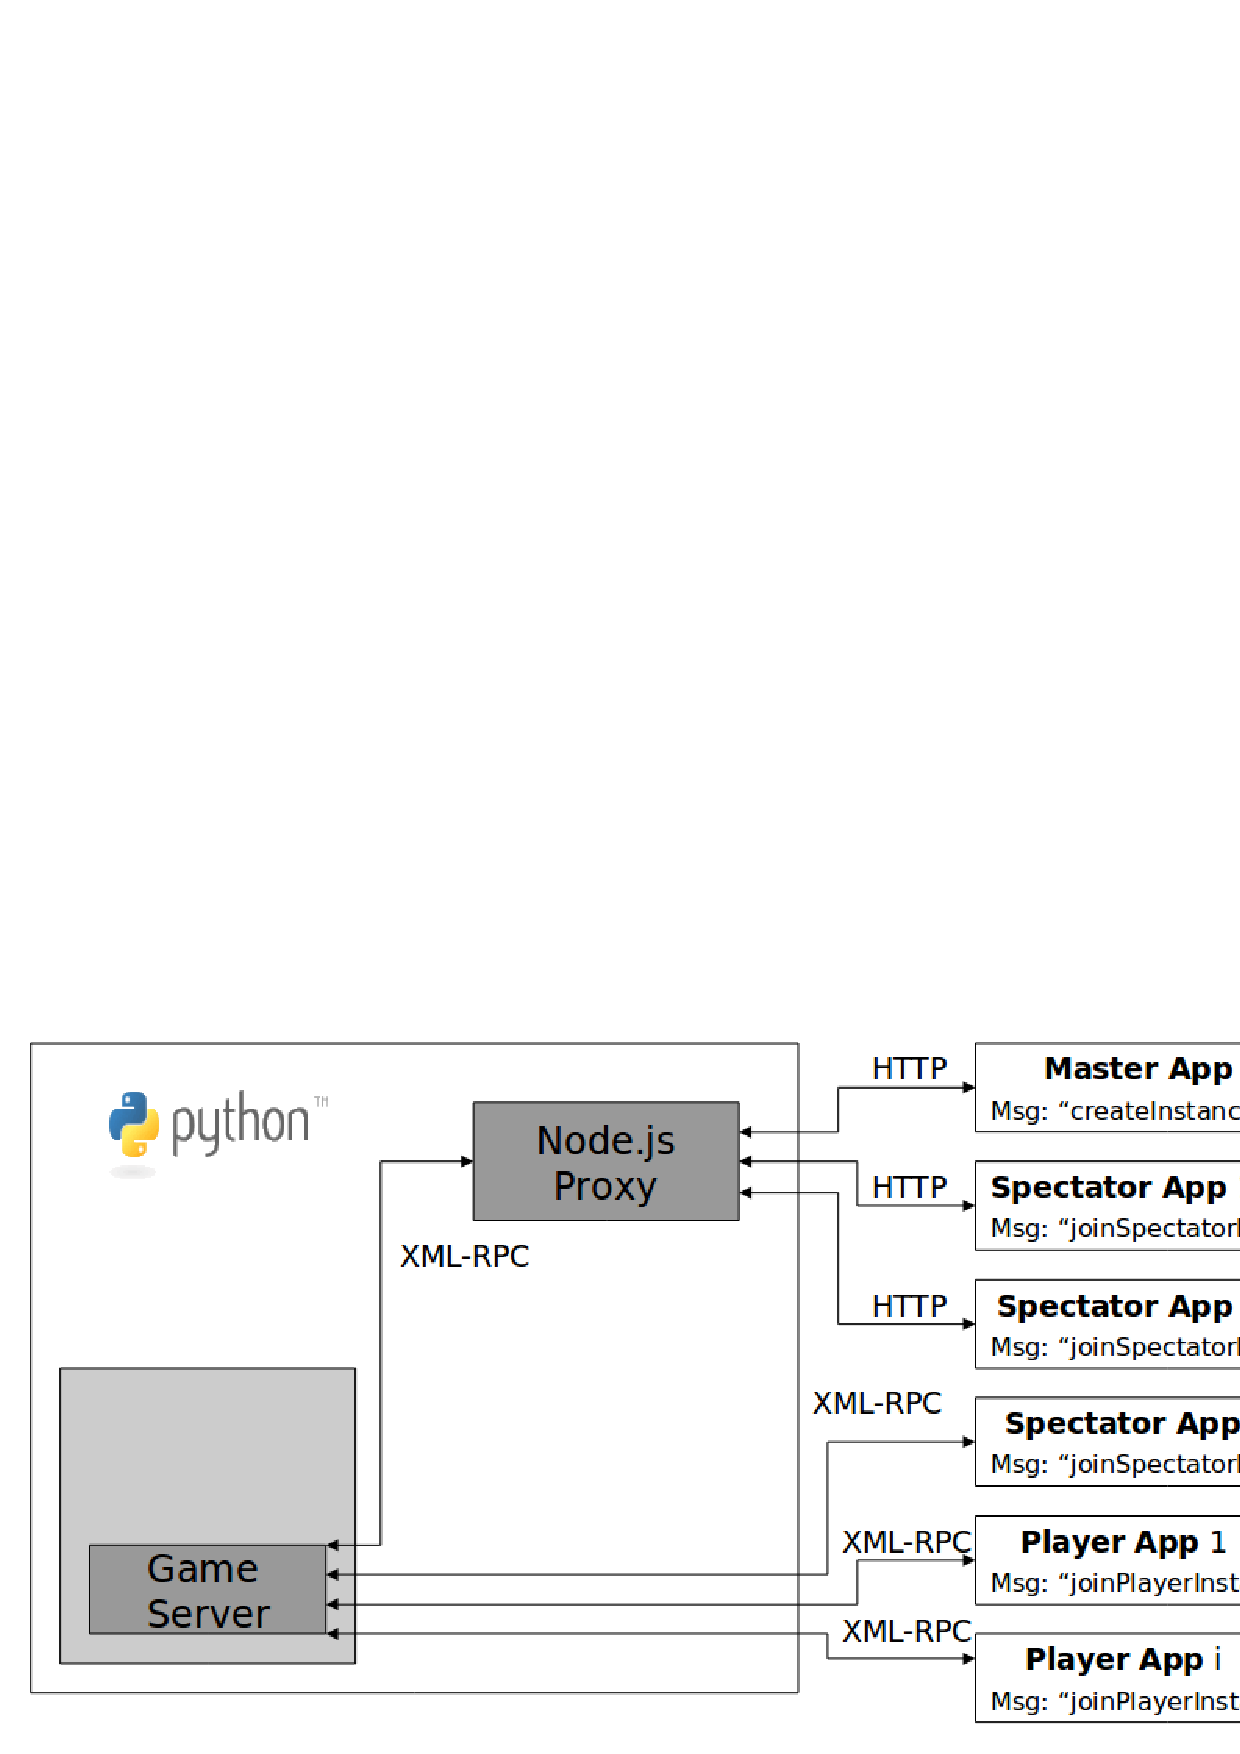
\includegraphics[scale=0.6]{Figures/_step1_xmlrpc}
\caption{System architecture with a focus on the login phase using XML-RPC}
\label{F_step1_xmlrpc}
\end{center}
\end{figure}


\begin{figure}[htbp!]
\begin{center}
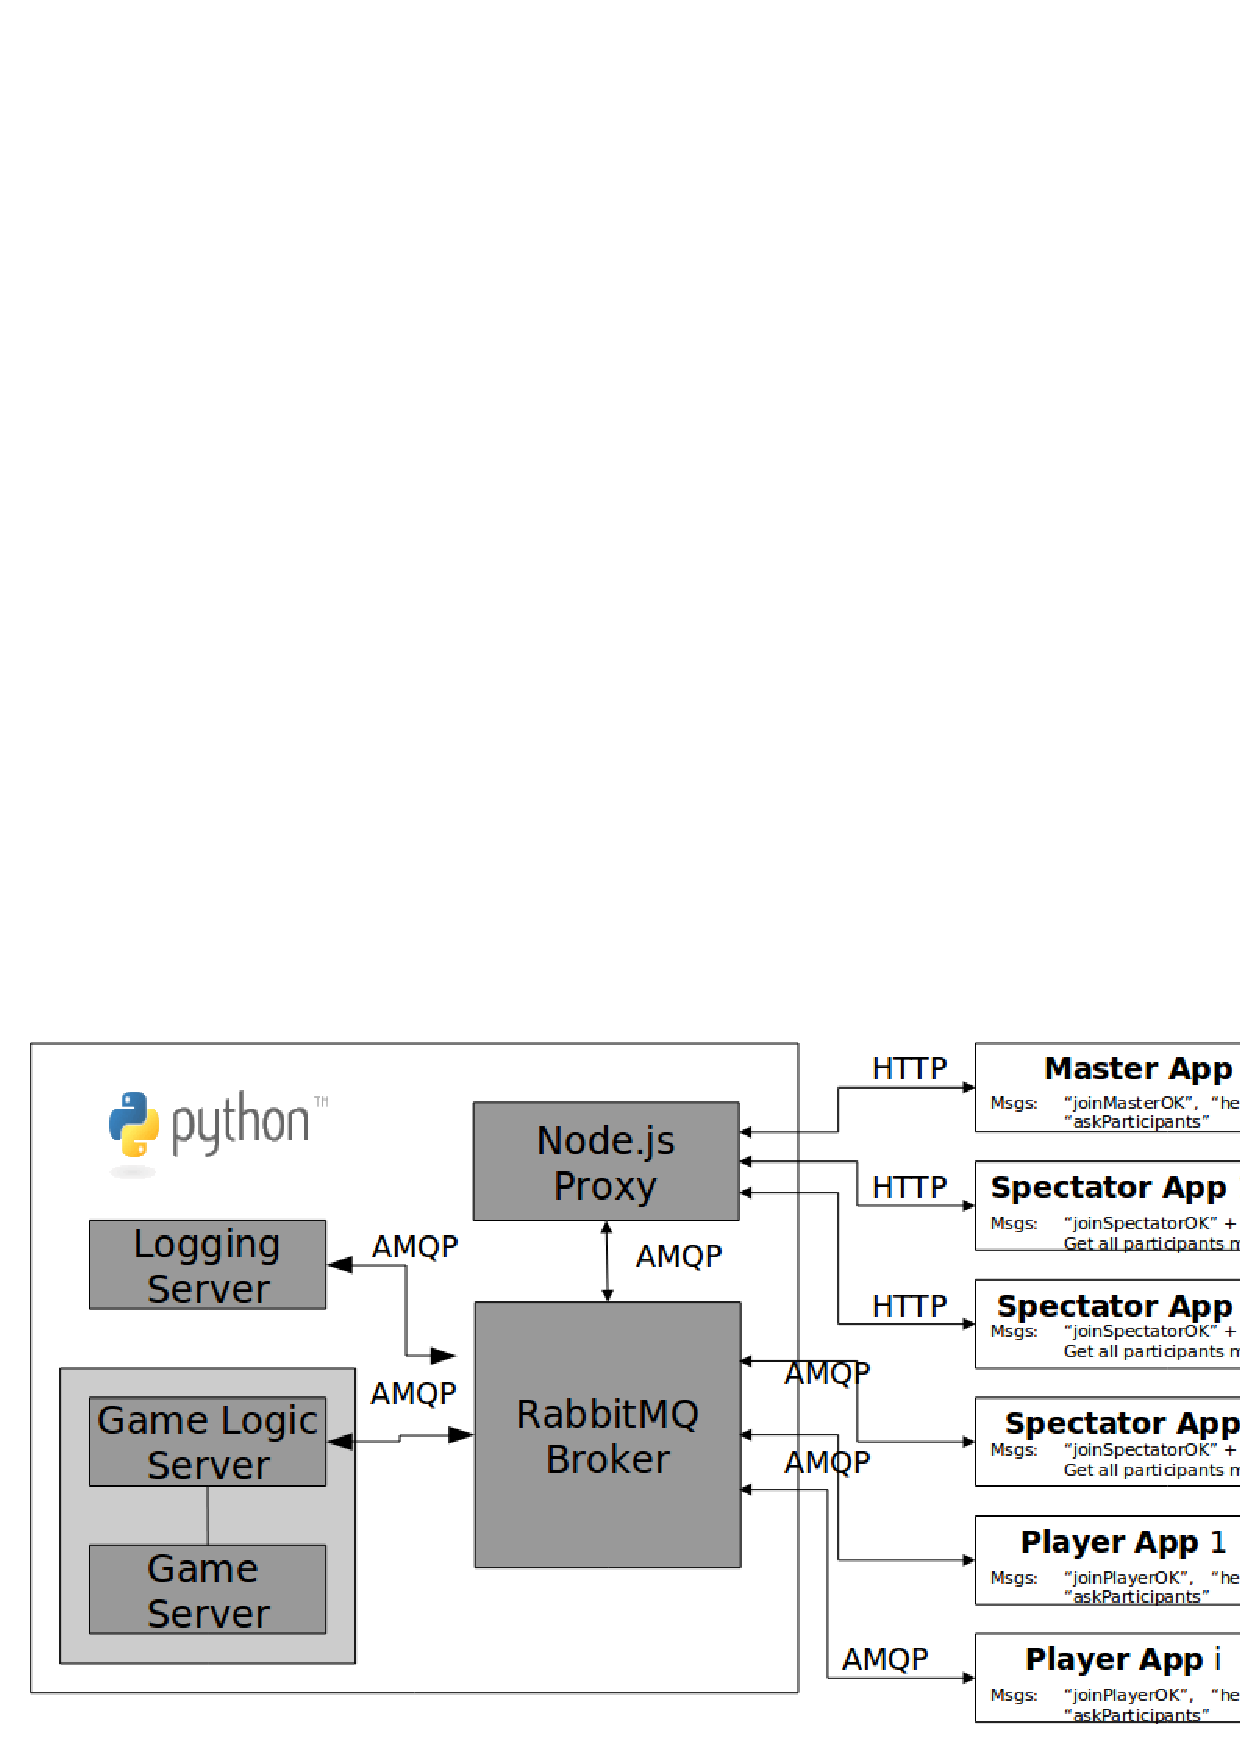
\includegraphics[scale=0.6]{Figures/_step2_amqp}
\caption{System architecture with a focus on the exchanging of messages using 
AMQP}
\label{F_step2_amqp}
\end{center}
\end{figure}

\endinput

\newpage
% TCM: TOTEM Communication Middleware
% Copyright: Copyright (C) 2009-2012
% Contact: denis.conan@telecom-sudparis.eu, michel.simatic@telecom-sudparis.eu
% Permission is granted to copy, distribute and/or modify this document
% under the terms of the GNU Free Documentation License, Version 1.3
% or any later version published by the Free Software Foundation;
% with no Invariant Sections, no Front-Cover Texts, and no Back-Cover Texts.
% A copy of the license is included in the section entitled "GNU
% Free Documentation License".

\section{Detailed design of the communication infrastructure}
\label{S_detailed_design}

This section details the design of the communication infrastructure:
the part built over the XMLRPC standard
(cf.~Figure~\ref{F_architecture_game_server}) and the part built over
the AMQP standard (cf.~Figure~\ref{F_architecture_game_instance}).

In Figure~\ref{F_architecture_game_server}, the game server receives
the login calls of the end-users. The game master calls for the
creation of the game instance. When created, the game logic server
of the game instance receives the calls forwarded by the game server
for opening the connection to the AMQP channels. At the end of the
creation and login phase, the AMQP communication infrastructure is as
depicted in Figure~\ref{F_architecture_game_instance}.

The design decisions concerning AMQP resources are the following ones:
\begin{itemize}
\item Every entity that communicates with the broker, either end-user 
applications (PlayerApplication, MasterApplication...) or processes (GameServer,
 LoggingServer...) matches with an AMQP user on the broker side. As a game 
instance is represented by a virtual host, permissions are granted to users to
access the instance(s) they are logged in. Game instances are contained into 
distinct partitions, without any possible 
inter-communication. However, a user can repeat its login procedure in 
several game instances. It can then be able to communicate separately 
to several game instances.

\item A topic exchange is used by the GameLogicServer in order to enable the 
macthing between messages and routing keys. The routing key policy used by the 
middleware associates each message to a sender, a recipient, an action kind and 
an action name. Furthermore, with the meta-characters ``*'' and ``\#'', it is 
quite easy to enable broadcast communication, or subscription to all the users' 
queues.

\item For each user, a queue is declared and named with the user's login 
name. The queue is then
bound to the topic exchange GameInstance. For example, a queue named \textit{
Player1} is declared for user Player1. This queue is bound to the exchange 
GameInstance with the routing key \texttt{*.Player1.*.*}. 
It can be understood as ``receive all the messages from any sender which are 
for Player1''. Acknowledgment flags of 
queues are set to true: this means that the broker won't send any other message
to a client as long as the previous one hasn't been acknowledged. This property 
is particularly useful for the \textsf{Node.js} proxy: if the proxy crashes, 
all the messages for a JavaScript client stay on the broker side.

\end{itemize}

\begin{figure}[htbp!]
\begin{center}
\includegraphics[scale=0.80,angle=90]{Figures/architecture_game_server}
\caption{Architecture of the XML-RPC communication infrastructure}
\label{F_architecture_game_server}
\end{center}
\end{figure}

\begin{figure}[htbp!]
\begin{center}
\includegraphics[scale=0.7,angle=90]{Figures/architecture_game_instance}
\caption{Architecture of the AMQP communication infrastructure}
\label{F_architecture_game_instance}
\end{center}
\end{figure}

The design and implementation decisions concerning AMQP message
exchanges:
\begin{itemize}
\item The style of programming is by exchanging messages and reacting
  to messages. This is ensured by the use of a state machine. In the sequel of 
  the document, the protocols of the state
  machines are sequences of messages with their type and content, and
  the reactions are the actions executed when receiving messages.
\item The Python TOTEM library is dedicated to the
  applications running on the game logic server and the logging
  server, thus using Pika in the continuous-passing programming style
  (with callbacks) in order to better scale.
\item The Java TOTEM library is dedicated to mobile Android
  applications, thus using the \textsf{RabbitMQ} Java Client with the
  blocking-calls programming style in order to limit multithreading
  and asynchrony.
\item The JavaScript TOTEM library is dedicated to Web applications, 
and communicates with the RabbitMQ broker through a proxy. The proxy itself is 
built with the JavaScript framework \textsf{Node.js}, which uses an AMQP library
 to 
publish and consume messages from the broker. Messages received by the proxy and
dedicated to a particular Web application are retrieved by this application via
AJAX requests using long polling. To publish messages, Web 
applications send them to the proxy in GET requests, and the proxy publishes 
those messages to the broker on the AMQP connection matching the Web 
application.
\item Python, Java and JavaScript idioms are built to obtain extensible state
  machines (cf.~Section~\ref{S_api}).
\item The GameLogicServer, which uses the Python library for AMQP Pika, cannot 
publish messages in separate threads, as the channel used is not thread-safe.
For Java and Android clients, with the version of the AMQP client used 
(2.7.0 or greater), there isn't anymore such a constraint. When using JavaScript, either on a Web application or on the Node.js proxy, there isn't such a constraint neither, since JavaScript is a single-threaded language.
\item As stated in the AMQP standard, when a problem
  happens, the connection is closed. In the Java
  TOTEM library, if an exception is thrown when connecting, publishing
  or consuming, then the connection is closed and re-opened in order
  to retry the operation (up to a maximum number of retries).
  For Web applications, a maximum number of retries is also given, but
  it is only used for the consumption of messages. If a disconnection 
  between the application and the proxy occurs, the Web application tries to
  reconnect to the proxy to receive messages until the maximum number of 
retries is reached. For the publication
  of messages, it's up to the Web browser to ensure the sending of the GET 
  request as soon as the network is reachable again.

\end{itemize}

The limitations of the current design and implementation, which
correspond to the example application described in
Section~\ref{S_integration}, are the following ones:
\begin{itemize}
\item No tests have been performed with several game logic servers. In
  the example application described in Section~\ref{S_integration},
  there is one virtual host for the game logic server of the sole game
  instance.
\item There is no defense programming such as checking whether the
  game instance is already created / started, the user (game master,
  player, or spectator) has already joined the game instance, a
  spectator is already a player. These kinds of verifications are business
application specific and should
  for instance lead to the definition of many new message types and
  exception classes.
\end{itemize}

\endinput

\newpage
% TCM: TOTEM Communication Middleware
% Copyright: Copyright (C) 2009-2012
% Contact: denis.conan@telecom-sudparis.eu, michel.simatic@telecom-sudparis.eu
% Permission is granted to copy, distribute and/or modify this document
% under the terms of the GNU Free Documentation License, Version 1.3
% or any later version published by the Free Software Foundation;
% with no Invariant Sections, no Front-Cover Texts, and no Back-Cover Texts.
% A copy of the license is included in the section entitled "GNU
% Free Documentation License".


\section{API of the communication infrastructure}
\label{S_api}

The API of the communication infrastructure using \textsf{RabbitMQ} is
provided in Java for Android and J2SE, in JavaScript for Web applications, 
and in Python for the the GameServer, the GameLogicServer and the LoggingServer.
 Section~\ref{SS_api_android} presents the API for Android
clients, Section presents the API for JavaScript clients, and 
Section~\ref{SS_api_python} presents the API for Python
clients.

% TCM: TOTEM Communication Middleware
% Copyright: Copyright (C) 2009-2012
% Contact: denis.conan@telecom-sudparis.eu, michel.simatic@telecom-sudparis.eu
% Permission is granted to copy, distribute and/or modify this document
% under the terms of the GNU Free Documentation License, Version 1.3
% or any later version published by the Free Software Foundation;
% with no Invariant Sections, no Front-Cover Texts, and no Back-Cover Texts.
% A copy of the license is included in the section entitled "GNU
% Free Documentation License".


\subsection{Android Java idioms for player, game master and spectator
applications}
\label{SS_api_android}

\textit{The idioms are the same for player, game master and spectator applications. But depending on client application, some class names vary. For example, 
the class GameMasterState is called 
PlayerState for the player application and SpectatorState for the 
spectator application. In this section, we provide the idioms for the 
PlayerMasterAndroid.}

\subsubsection{Class \texttt{PlayerApplication}}

The class \texttt{PlayerApplication} is the \texttt{Activity} of the Android 
application. It is used to:

\begin{enumerate}
\item Load configuration data from the file \texttt{xmlrpc.properties}:
\begin{small}
\begin{alltt}
gameServerXMLRPCHost        localhost
gameServerXMLRPCPort        8888
[...]
\end{alltt}
\end{small}
\item Load configuration data from the file \texttt{rabbit.properties}:
\begin{small}
\begin{alltt}
gameServerUserName          gameserver
gameLogicServerUserName	    gamelogicserver
loggingServerUserName       loggingserver

gameLogicServerBrokerHost   localhost
gameLogicServerBrokerPort   5672
gameLogicServerExchangeType topic
gameLogicServerExchangeName GameInstance
[...]
\end{alltt}
\end{small}
\item Create and set the logger, used to display log messages on the device 
screen:
\begin{small}
\begin{alltt}
Util.setLogger(this);
\end{alltt}
\end{small}
\item Execute the \texttt{PlayerTask}
\begin{small}
\begin{alltt}
playerTask = new PlayerTask(PlayerApplication.this);
playerTask.execute();
\end{alltt}
\end{small}
\end{enumerate}

\subsubsection{Class \texttt{PlayerTask}}


The class \texttt{PlayerTask} allows to execute the XML-RPC call for the login 
and to compute the response of the GameServer. Note that we have decided to 
make this class extend the class AsyncTask of the Android SDK to enable the 
displaying of information messages during the XML-RPC call. However, if you 
consider that such messages are not required by your application, you can 
organize your code without a class extending AsyncTask.
The class \texttt{PlayerTask} consists in the following steps:

\begin{enumerate}

\item Log-in to the game server, and either create a game instance by an 
XML-RPC call of the method \texttt{createGameInstance} or join an existing game
instance by an XML-RPC call of the method \texttt{joinGameInstance}.
\item Create the game logic state managed by the client application:
\begin{small}
\begin{alltt}
state = new PlayerState();
\end{alltt}
\end{small}
\item Instantiate the ChannelManager to communicate with the broker and
assign the game logic state and the lists of actions of
  the state machine of the client:
\begin{small}
\begin{alltt}
state.channel = ChannelsManager.getInstance(state,
                                                MyListOfGameLogicActions.ListOfActionsMaps);
\end{alltt}
\end{small}
\item Publish a message for announcing the joining to
  the broker, the second argument being the content
  of the message (\emph{e.g.}, \texttt{``Publish the String "lisa,mygamename,myinstancename"''}):
\begin{small}
\begin{alltt}
state.channel.publishToGameLogicServer(state,
                                       JoinAction.JOIN\_PLAYER,
                                       state.login
                                       + ....getProperty("bodySeparator")
                                       + state.gameName
                                       + ....getProperty("bodySeparator")
                                       + state.gameInstanceName);
\end{alltt}
\end{small}
\end{enumerate}

\subsubsection{State machine enumeration type for the game logic of the player}

The state machine for the game logic is specified into two sorts of
enumeration types: the first sort enumeration type specifies the
lists of action kinds
(cf.~Listing~\ref{L-applicationinstanceactionkinds}) and the second
enumeration type specifies the actions per action kinds
(cf.~Listing~\ref{L-applicationinstanceactionsone}
and~Listing~\ref{L-applicationinstanceactionstwo}). The protocol of the game 
logic specified in the TOTEM library is complemented by the list of actions 
specified in these classes.

\begin{lstlisting}[float=htbp,frame=bt,basicstyle=\scriptsize\sffamily,numbers=left,
   numberstyle=\tiny, stepnumber=1,
    numbersep=5pt,language=java,label=L-applicationinstanceactionkinds,caption=List of action kinds of the state machine for the game logic of the player]
public enum MyListOfGameLogicActions {
  MY_FIRST_ACTION_KIND(MyFirstActionKind.actionMap),
  MY_SECOND_ACTION_KIND(MySecondActionKind.actionMap);
	
	// Ignore the code below. Just make sure it is present in all your enums.
	// The copy and paste is due to a limitation of Java enums (no inheritance).
\end{lstlisting}

\begin{lstlisting}[float=htbp,frame=bt,basicstyle=\scriptsize\sffamily,numbers=left,
   numberstyle=\tiny, stepnumber=1,
    numbersep=5pt,language=java,label=L-applicationinstanceactionsone,caption=Player's actions of the first action kind]
public enum MyFirstActionKind implements PlayerActionInterface {
  MY_FIRST_ACTION("myFirstAction") {
    public Object execute(PlayerState state, String[] header, String body)
        throws ActionInvocationException {
      return MyGameLogicProtocol.myFirstAction(state, header,body);
    }
  },
  MY_SECOND_ACTION("mySecondAction") {
    public Object execute(PlayerState state, String[] header, String body)
        throws ActionInvocationException {
      return MyGameLogicProtocol.mySecondAction(state, header, body);
    }
  },
  MY_THIRD_ACTION("myThirdAction") {
    public Object execute(PlayerState state, String[] header, String body)
        throws ActionInvocationException {
      return null;
    }
  };
  public final static int KIND_NUMBER = 100;
  public final static int LOWER_ACTION_NUMBER = 0;
  public final static int UPPER_ACTION_NUMBER = 1000;
  // Ignore the code below. Just make sure it is present in all your enums.
  // The copy and paste is due to a limitation of Java enums (no inheritance).
  [...]
}
\end{lstlisting}

\begin{lstlisting}[float=htbp,frame=bt,basicstyle=\scriptsize\sffamily,numbers=left,
   numberstyle=\tiny, stepnumber=1,
    numbersep=5pt,language=python,label=L-applicationinstanceactionstwo,caption=Player's actions of the second action kind]
public enum MySecondApplicationInstanceActionKind implements PlayerActionInterface {
  MY_FOURTH_ACTION("myFourthAction") {
    public Object execute(PlayerState state, String[] header, String body)
        throws ActionInvocationException {
      return MyGameLogicProtocol.myFourthAction(state, header, body);
    }
  },
  MY_FIFTH_ACTION("myFitfhAction") {
    public Object execute(PlayerState state, String[] header, String body)
        throws ActionInvocationException {
      return null;
    }
  };
  public final static int KIND_NUMBER = 101;
  public final static int LOWER_ACTION_NUMBER = 0;
  public final static int UPPER_ACTION_NUMBER = 1000;
  // Ignore the code below. Just make sure it is present in all your enums.
  // The copy and paste is due to a limitation of Java enums (no inheritance).
  [...]
}
\end{lstlisting}

\subsubsection{Game logic protocol of the state machine}

In Listing~\ref{L-applicationinstanceprotocol}, the protocol of the
state machine for the game logic is specified as a set of static
methods with three arguments: the state of the client, the header of
the message received and the content of the message. The
header of the message is the routing key of the message: four strings
indicating the emitter, the addressee, the action kind and the action.

\begin{lstlisting}[float=htbp,frame=bt,basicstyle=\scriptsize\sffamily,numbers=left,
   numberstyle=\tiny, stepnumber=1,
    numbersep=5pt,language=java,label=L-applicationinstanceprotocol,caption=Game logic's protocol of the state machine for the game logic]
public class MyGameLogicProtocol {
  public static Object myFirstAction(PlayerState state, String[] header, String body) {
    Util.println("Player" + state.login + "]" + body);
    return null;
  }
  public static Object mySecondAction(PlayerState state, String[] header, String body) {
    Util.println("[Player" + state.login + "]" + body);
    return null;
  }
  public static Object myFourthAction(PlayerState state, String[] header, String body) {
    Util.println("[Player" + state.login + "]" + body);
    return null;
  }
}
\end{lstlisting}

\subsubsection{Game logic state}

The game logic state is defined in the TOTEM library and can be
extended by client applications. All the attributes presented in
Listing~\ref{L-applicationinstancestate} are public.

\begin{lstlisting}[float=htbp,frame=bt,basicstyle=\scriptsize\sffamily,numbers=left,
   numberstyle=\tiny, stepnumber=1,
    numbersep=5pt,language=java,label=L-applicationinstancestate,caption=Player's state of the state machine]
public class PlayerState {
    public String    login;
    public String    password;
    public String    gameName;
    public String    gameInstanceName;
    public String    virtualHost;
    public String    exchangeName;
    public ChannelsManager channelsManager;
    public int       numberOfRetries;
    public boolean   hasConnectionExited;
    connectionExit();
}
\end{lstlisting}

\endinput

% TCM: TOTEM Communication Middleware
% Copyright: Copyright (C) 2009-2012
% Contact: denis.conan@telecom-sudparis.eu, michel.simatic@telecom-sudparis.eu
% Permission is granted to copy, distribute and/or modify this document
% under the terms of the GNU Free Documentation License, Version 1.3
% or any later version published by the Free Software Foundation;
% with no Invariant Sections, no Front-Cover Texts, and no Back-Cover Texts.
% A copy of the license is included in the section entitled "GNU
% Free Documentation License".

\subsection{JavaScript idioms for game master and spectator applications}
\label{SS_api_JavaScript}

\textit{The idioms are the same for game master and spectator applications. 
Here, we just provide the idioms for the game master application.}

\subsubsection{\texttt{master.js} file}

The master.js file represents the game master application, and uses
the TOTEM API in JavaScript. It consists in the following steps:

\begin{enumerate}

\item Loggin to the game server, and creation of a game instance by an 
XMLRPC to the method \texttt{createGameInstance}.
\item Creation the game logic state managed by the client application:
\begin{small}
\begin{alltt}
gameMasterState = new State(``login'',''password'',''gameName'',''instanceName'');
\end{alltt}
\end{small}
\item Implementation of the \texttt{onExitConnection()} function triggered by 
the API when the connection exits:
\begin{small}
\begin{alltt}
function onExitConnection()\{
  // update the display to show the end screen
  showEnd(); 
\}
\end{alltt}
\end{small}
\item Publish the message for announcing the joigning to
  the game instance broker, the second argument being the content body
  of the message (\emph{e.g.}, \texttt{lisa,mygamename,myinstancename}):
\begin{small}
\begin{alltt}
publishToGameLogicServer(gameMasterState, "join.joinMaster", "lisa,Tidy-City,Instance-1");
\end{alltt}
\end{small}
\end{enumerate}

\subsubsection{State machine actions for the game logic}

The state machine for the game logic is specified into actions kinds and 
actions. Actions kinds can be considered as name spaces to facilitate usage 
of actions. Listing~\ref{L-javascriptactionkinds} gives an example. Please refer to section \ref{SSS_actions} for further details.


\begin{lstlisting}[float=htbp,frame=bt,basicstyle=\scriptsize\sffamily,numbers=left,
   numberstyle=\tiny, stepnumber=1,
    numbersep=5pt,language=python,label=L-javascriptactionkinds,caption=GameMaster's actions of the first action kinds]
function MyFirstActionKind () {}

MyFirstActionKind.prototype.myFirstAction = function (state, publisher, consumer, message){
        println("My first action","Message received from "+publisher+": "+message);
};
\end{lstlisting}

Such an action kind have to be declared to the game logic state:
\begin{small}
\begin{alltt}
gameMasterState.listOfActions.myFirstActionKind = new MyFirstActionKind();
\end{alltt}
\end{small}

\subsubsection{Game logic's State class}

The game logic's State class is defined in the TOTEM library. All the attributes presented in
Listing~\ref{L-gamemasterstatejs} are public.

\begin{lstlisting}[float=htbp,frame=bt,basicstyle=\scriptsize\sffamily,numbers=left,
   numberstyle=\tiny, stepnumber=1,
    numbersep=5pt,language=python,label=L-gamemasterstatejs,caption=GameMaster's state]
function State(login, password, gameName, instanceName, heartbeat, maxRetry){
    this.login = login;
    this.password = password;
    this.gameName = gameName;
    this.instanceName = instanceName;
    if (typeof heartbeat == "number"){
        this.heartbeat = heartbeat;
    }else{
        this.heartbeat = DEFAULT_HEARTBEAT_TASK_PERIOD;
    }
    if (typeof maxRetry == "number"){
        this.maxRetry = maxRetry;
    }else{
        this.maxRetry = DEFAULT_MAX_RETRY;
    }
    this.listOfActions = {  join: new JoinAction(),
                            presence: new PresenceAction(),
                            lifecycle: new LifeCycleAction()};
    [...]
}
\end{lstlisting}

\endinput

% TCM: TOTEM Communication Middleware
% Copyright: Copyright (C) 2009-2012
% Contact: denis.conan@telecom-sudparis.eu, michel.simatic@telecom-sudparis.eu
% Permission is granted to copy, distribute and/or modify this document
% under the terms of the GNU Free Documentation License, Version 1.3
% or any later version published by the Free Software Foundation;
% with no Invariant Sections, no Front-Cover Texts, and no Back-Cover Texts.
% A copy of the license is included in the section entitled "GNU
% Free Documentation License".


\subsection{Python idioms for the game logic server}
\label{SS_api_python}

This section details only the idioms for the game logic server. The protocol 
of the game logic server specified in the TOTEM library is
complemented by the list of actions specified in the listings~\ref{L-listofactions}, \ref{L-firstactionkind}, and \ref{L-secondactionkind}.

\begin{lstlisting}[float=htbp,frame=bt,basicstyle=\scriptsize\sffamily,numbers=left,
   numberstyle=\tiny, stepnumber=1,
    numbersep=5pt,language=python,label=L-listofactions,caption=List of action kinds of the state machine for the game logic server]
MyListOfActions = ListOfActionsEnumeration("MyListOfActions",
    [("myFirstActionKind", MyFirstActionKind),
     ("mySecondActionKind", MySecondActionKind)
     ])
\end{lstlisting}

\begin{lstlisting}[float=htbp,frame=bt,basicstyle=\scriptsize\sffamily,numbers=left,
   numberstyle=\tiny, stepnumber=1,
    numbersep=5pt,language=python,label=L-firstactionkind,caption=Game logic server's actions of the first action kinds]
def doNothing(state, header, body):
    pass

MyFirstActionKind = GameLogicActionEnumeration("myFirstActionKind", 100, 0, 1000,
    [("myFirstAction", myFirstAction),
     ("mySecondAction", mySecondAction),
     ("myThirdAction",doNothing)
     ])
\end{lstlisting}

\begin{lstlisting}[float=htbp,frame=bt,basicstyle=\scriptsize\sffamily,numbers=left,
   numberstyle=\tiny, stepnumber=1,
    numbersep=5pt,language=python,label=L-secondactionkind,caption=Game logic server's actions of the second action kinds]
def doNothing(state, header, body):
    pass

MySecondActionKind = GameLogicActionEnumeration("mySecondActionKind", 101, 0, 1000,
    [("myFourthAction", myFourthAction),
     ("myFitfhAction", myFitfhAction)
     ])
\end{lstlisting}


\subsubsection{Game logic server state}

The game logic server's state is defined in the TOTEM library and can be
extended by client applications. All the attributes presented in
Listing~\ref{L-gamelogicserverstate} are public.

\begin{lstlisting}[float=htbp,frame=bt,basicstyle=\scriptsize\sffamily,numbers=left,
   numberstyle=\tiny, stepnumber=1,
    numbersep=5pt,language=python,label=L-gamelogicserverstate,caption=Game logic server's state]
class MyState(GameLogicState):
    mynewstatevariable = None
class GameLogicState(object):
    createGameInstanceSemaphore = None
    vhost = None
    connection = None
    channel = None
    gamelogiclistofactions = None
    gameName = None
    instanceName = None
\end{lstlisting}


\subsubsection{Game logic server's protocol of the state machine}

In Listing~\ref{L-gamelogicserverprotocol}, the protocol of the state
machine for the game logic server is specified as methods with three
arguments: the state of the game logic server, the header of the
message received and the content of the message.

\begin{lstlisting}[float=htbp,frame=bt,basicstyle=\scriptsize\sffamily,numbers=left,
   numberstyle=\tiny, stepnumber=1,
    numbersep=5pt,language=python,label=L-gamelogicserverprotocol,caption=Game logic server's protocol of the state machine]
def myFirstAction(state, header, body):
    print ' [GameLogicServer] React to myFirstAction message'

def mySecondAction(state, header, body):
    print ' [GameLogicServer] React to mySecondAction message'

def myFourthAction(state, header, body):
    print ' [GameLogicServer] React to myFourthAction message'

def myFitfhAction(state, header, body):
    print ' [GameLogiceServer] React to myFitfhAction message'
\end{lstlisting}

\endinput


\endinput

\newpage
% TCM: TOTEM Communication Middleware
% Copyright: Copyright (C) 2009-2012
% Contact: denis.conan@telecom-sudparis.eu, michel.simatic@telecom-sudparis.eu
% Permission is granted to copy, distribute and/or modify this document
% under the terms of the GNU Free Documentation License, Version 1.3
% or any later version published by the Free Software Foundation;
% with no Invariant Sections, no Front-Cover Texts, and no Back-Cover Texts.
% A copy of the license is included in the section entitled "GNU
% Free Documentation License".

\section{Organisation of the source code}
\label{S_sourcecode}

The source code provided into the directory structure
\textsf{TOTEM.CommunicationMiddleware/Sources} is organised as
follows. Every directory contains a file \texttt{readme.txt}.

\begin{small}
\begin{alltt}

Sources
|-- IntegrationExampleApplication      \textit{# application presented in Section 9}
|   |-- GameLogicServer                \textit{# game logic of the game}
|   |-- GameServer                     \textit{# Python server part managing the broker}
|   |-- MasterApplication              \textit{# J2SE game master application}
|   |-- MasterApplicationJavascript    \textit{# Javascript game master application}
|   |-- NodeJsProxy                    \textit{# Node.js proxy used by Javascript applications}
|   |-- PlayerApplication              \textit{# J2SE player application}
|   |-- PlayerMasterAndroid            \textit{# Java Android application acting both as player and master}
|   |-- SpectatorApplication           \textit{# J2SE spectator application}
|   |-- SpectatorApplicationJavascript \textit{# Javascript spectator application}
|   `-- TerminationApplication         \textit{# Python application to call for termination}
|-- RabbitMQTOTEMLibrary               \textit{# Code extracted to be in the TOTEM library}
|   |-- Java
|   |   |-- common
|   |   |-- gamemasterapplication
|   |   |-- playerapplication
|   |   `-- spectatorapplication
|   |-- JavaScript
|   |    `-- external
|   `-- Python
|       `-- eu
|           `-- telecomsudparis
|               `-- rabbitmq
|                   |-- applicationinstance
|                   `-- configuration
`-- TutorialExamples       \textit{# RabbitMQ tutorial, cf. http://www.rabbitmq.com/getstarted.html}
    |-- Android
    |   |-- Step1, |-- Step2, |-- Step3, |-- Step4, |-- Step5, `-- Step6
    |-- J2SE
    |   |-- Step1, |-- Step2, |-- Step3, |-- Step4, |-- Step5, `-- Step6
    |-- Javascript
    |   |-- Step1, |-- Step2, |-- Step3, |-- Step4, |-- Step5, `-- Step6
    `-- Pika
        |-- Step1, |-- Step2, |-- Step3, |-- Step4, |-- Step5, `-- Step6

\end{alltt}
\end{small}

\endinput

\newpage
% TCM: TOTEM Communication Middleware
% Copyright: Copyright (C) 2009-2012
% Contact: denis.conan@telecom-sudparis.eu, michel.simatic@telecom-sudparis.eu
% Permission is granted to copy, distribute and/or modify this document
% under the terms of the GNU Free Documentation License, Version 1.3
% or any later version published by the Free Software Foundation;
% with no Invariant Sections, no Front-Cover Texts, and no Back-Cover Texts.
% A copy of the license is included in the section entitled "GNU
% Free Documentation License".


\section{Tutorial: understanding the concepts of the middleware to publish and 
consume messages}
\label{S_tutorialprotocol}

This section is a tutorial for explaining the concepts of the
middleware and of its client applications (located in the directory
\texttt{TOTEM.CommunicationMiddleware/Sources/IntegrationExampleApplication}
of the TOTEM SVN), and the use of those concepts to publish and
consume GPS coordinates using the AMQP part of the TOTEM Communication
Middleware. It is also the opportunity to briefly presents the
different XML-RPC methods used to interact with the game server.

\subsection{In a nutshell}
\label{SS_nutshell}

\subsubsection{Game server and Game Logic server}

A client of the middleware can communicate with two different 
entities: the Game server and the Game Logic server. The Game 
server represents the lobby (term used in the jargon 
of multiple-players video games): it allows the listing, the creation, 
the joining and the termination of game instances. The Game 
Logic server represents a single game instance. Two different
protocols should be used depending on the entity to communicate with: 
communication with the Game server is ensured by XML-RPC calls, whereas 
communication with the Game Logic server is based on AMQP.

\subsubsection{Interacting with the game server using XML-RPC}

A client should first either create a game instance, or list the already 
existing game instances and join one. To perform the XML-RPC calls, a 
Java/Android application calls the Game server
using XML-RPC. For JavaScript applications, the methods are 
provided by the API: they allow to send a request to the Node.js proxy which 
executes the XML-RPC calls to the GameServer. Here follows the methods that can 
be called on the Game server:

\begin{itemize}
\item 
\begin{shellcmd} 
Object[] listGameInstances(gameName)
\end{shellcmd} 
 to retrieve the list of existing instances for a given game (Object[]
 for Java clients, whose elements can be cast in String - tuple for
 Android and JavaScript clients);
\item 
\begin{shellcmd}
Boolean createGameInstance(login, password, gameName,instanceName)
\end{shellcmd} 
to create a game instance for a given game, and to join it;
\item 
\begin{shellcmd}
Boolean joinPlayerGameInstance(login, password, gameName, instanceName)
\end{shellcmd} 
to make a player application (Java or Android) join an existing game instance;
\item 
\begin{shellcmd}
Boolean joinSpectatorGameInstance(login, password,gameName,instanceName, observationKey)
\end{shellcmd} 
to make a spectator application (Java or JavaScript) join an existing game
instance ,observationKey is used to filter messages to consume;
\item 
\begin{shellcmd}
Boolean terminateGameInstance(gameName, instanceName)
\end{shellcmd} 
to terminate a given instance of a given game;
\item 
\begin{shellcmd}
Boolean terminate()
\end{shellcmd} 
to terminate the game server, and hence every existing game
instances. Note: clients don't need special permissions to call this
method.
\end{itemize}

\subsubsection{Publishing messages}

Once a client has joined a game instance, the publication and the
consumption of messages within the game instance is ensured using the
AMQP protocol. The TOTEM Communication Middleware provides high-level
methods hiding the complexity of AMQP.

Messages can be published to a given user (designed by its login) or
to the Game Logic server, or can be broadcast to all the users of a
game instance and to the Game Logic server. The three matching
(publish, publishToGameLogicServer, publishToAll)
publication methods use the following parameters:
\begin{itemize}
\item the \textbf{state} of the state machine of the user, which
  contains the information required for the publication of a
  message (login, game name, instance name...),
\item a String representing the \textbf{content} of the message,
\item an \textbf{action kind} and an \textbf{action}. Their role is described 
in Section \ref{SSS_actions}. 
\end{itemize}

As it is already mentioned in Section \ref{S_detailed_design}, the
\textbf{Game Logic server programmed in Python should not publish
  messages in separate threads}, since the AMQP mechanism for the
publication of messages is not thread-safe. There isn't such
limitation on Java Android and JavaScript applications.


\subsubsection{Computing messages: actions and action kinds}
\label{SSS_actions}
Since clients of the TOTEM Communication Middleware don't have to
handle the low-level details of reception of messages, they just need
to define a behaviour on the consumption of these messages. This is
why actions and action kinds are made for. An action represents a
particular behaviour, whereas an action kind defines a name space for
a set of actions of a whole protocol. When a client publish a message
to another client, it must give both the action kind and the action
matching with the message. When the other client consumes the message,
if the action kind and the action are defined on its state machine,
the corresponding method will automatically be triggered by the TOTEM
Communication Middleware. Otherwise, the messages are printed
nevertheless.  The implementation of actions and action kinds are
different for Java Android applications, JavaScript applications and
for the Game Logic server in Python (please refer to Chapter \ref{S_api}
for further details).  Let's see the example of a JavaScript
application which has defined the following action kind and action:
\begin{shellcmd}
function LocationActionKind () \{\}

LocationActionKind.prototype.sendCoordinates = function (state, publisher, consumer, message)\{ 
      println("Send coordinates action","New coordinates from "+publisher+": "+message); 
\};
\end{shellcmd}
and which has stored the action kind on its state machine:
\begin{shellcmd}
myState.listOfActions.LocationActionKind = new LocationActionKind();
\end{shellcmd}

From now, every client that publishes a message to this JavaScript
application, setting the action parameter of the publish method to
\texttt{"LocationActionKind.sendCoordinates"}
(\textsf{actionkind.action}) will trigger the execution of the
\texttt{sendCoordinates(state, publisher, consumer, message)} function
on the JavaScript application side.

\subsection{Publishing and consuming GPS coordinates}
\label{SS_sending_computing_GPS}

In Section \ref{SS_point_to_point_android}, a player
periodically publish a message to another player. On the consumption of
the message, the other player prints this message. In
Section \ref{SS_broadcast_gamelogic}, the player broadcast its
coordinates to the others players and to the game logic server. In
Section \ref{SS_broadcast_js}, the master application written in
JavaScript consumes the messages.

\subsubsection{Point to point communication between Android devices}
\label{SS_point_to_point_android}

In the Android project \texttt{PlayerMasterAndroid}:

\begin{enumerate}
\item Create new \textsf{actionKind} and \textsf{action} in a Java
  state machine:
\begin{itemize}
\item Copy the class \texttt{MyFirstActionKind} located in the package
\texttt{eu.telecomsudparis.integration.player.android}, paste it in the same
package, and rename it \texttt{LocationActionKind}. 
\newline
Note: If you are using an IDE like
Eclipse, every references to  \texttt{MyFirstActionKind} should be automatically
replaced by reference to \texttt{LocationActionKind}. Otherwise, you need to
replace those references by yourself.
\item In this new class:
\begin{itemize}
\item The value of the attribute \texttt{nameKind} is set to
  \texttt{"myFirstActionKind"}. Replace this value by
  \texttt{"locationActionKind"}.
\begin{itemize}
\item The action kind part of location messages is a string,
  for instance \texttt{player1.gamelogicserver.locationActionKind}
  followed by a string specifying the action.
\end{itemize}
\item The value of the attribute \texttt{KIND\_NUMBER} is to \texttt{100}. 
Replace this value by \texttt{102}.
\item The name of the first enum of the list is set to
  \texttt{MY\_FIRST\_ACTION("myFirstAction")}, Replace this name with
  \texttt{SEND\_GPS\_COORDINATES("sendGPSCoordinates")}.
\begin{itemize}
\item The action part of location messages is specified by that string,
  for instance
  \texttt{player1.gamelogicserver.locationActionKind.sendGPSCoordinates}.
\end{itemize}
\end{itemize}
\item The enumerations \texttt{MY\_SECOND\_ACTION("mySecondAction")} and
  \texttt{MY\_THIRD\_ACTION("myThirdAction")} can be removed. Note:
  Beware to keep a semicolon after the last enumeration, otherwise the source
  code does not compile.
\end{itemize}

\item Implement the required behaviour on the reception of the \textsf{action}:

\begin{itemize}
\item In the class \texttt{MyGameLogicProtocol}, add the following
  static method:
\begin{shellcmd}
public static Object computeGPSCoordinates(String player, String coordinates) \{
      Util.println(player+" GPS coordinates received : "+coordinates);
      return null;
\}
\end{shellcmd}
\item In the class \texttt{LocationActionKind}, complete the method
  \texttt{execute} of \texttt{SEND\_GPS\_COORDINATES}:
\begin{shellcmd}
public Object execute(PlayerState state, String[] header, String body) 
                     throws ActionInvocationException \{
    return MyGameLogicProtocol.computeGPSCoordinates(header[0],body);
\}
\end{shellcmd} 
\textit{Notice that \texttt{header[0]} refers to the sender of the message.}
\end{itemize}


\item Register the new \textsf{action kind} in the list of actions:
\begin{itemize}
\item Add a new enumeration in the class \texttt{MyListOfGameLogicActions},
  after MY\_FIRST\_ACTION\_KIND(MyFirstActionKind.actionMap) and
  MY\_SECOND\_ACTION\_KIND(MySecondActionKind.actionMap):
\begin{itemize}
\item \texttt{LOCATION\_ACTION\_KIND(LocationActionKind.actionMap);}
\end{itemize}
\end{itemize}

\item Simulate the publication of GPS coordinates:

\begin{itemize}
\item In the class \texttt{PlayerTask}, add the method presented in
  Listing \ref{L-GPS-thread}:
\begin{lstlisting}[float=htbp,frame=bt,basicstyle=\scriptsize\sffamily,numbers=left,
   numberstyle=\tiny, stepnumber=1,
    numbersep=5pt,language=java,label=L-GPS-thread,caption=Method to send simulated GPS coordinates]
// simulates the sending of GPS coordinates
private void startSendGPSCoordinatesThread() {
     new Thread(){
     double latitude  = -179.8642632;
     double longitude = -179.2570048;
     // the recipient is the other player
     String recipient = state.login.equals(PlayerApplication.INSTANCE_CREATOR_NAME) ? 
                                           PlayerApplication.INSTANCE_JOINER_NAME :
                                           PlayerApplication.INSTANCE_CREATOR_NAME;
     public void run() {
         while (!state.hasConnectionExited()){
	     try {
	         state.channelsManager.publish(recipient,
                                               state,
                                               LocationActionKind.SEND_GPS_COORDINATES, 
                                               latitude+"/"+longitude);
	         // increment the coordinates
	         latitude ++;
	         longitude ++;
	     } catch (IOException e) {
	         e.printStackTrace();
	     }
	     // wait for 5 seconds
	     try {
	        Thread.sleep(5000);
	     } catch (InterruptedException e) {
	        Util.println("[Player" + state.login + 
				"]Thread sleep was interrupted");
	     }
         }
     }
  }.start();
}
\end{lstlisting}
\item Complete the method \texttt{doInBackground(Void... params)} to make
the client which creates the instance calling this method:

\begin{shellcmd}
@Override
protected Integer doInBackground(Void... params) \{
    [...]
    if(res)\{
        if(state.login.equals(PlayerApplication.INSTANCE_CREATOR_NAME))\{
             startSendGPSCoordinatesThread();
        \}
        return RESULT_OK;
    \}else\{
        return RESULT_ERROR;
    \}
\}
\end{shellcmd}
\end{itemize}
\item Test the communication between two Android devices (or emulators):
\label{item_test}
\begin{enumerate}
\item Configure and start the Game server:
\begin{itemize}
\item Set the IP addresses of the GameServer and of the
  TerminationApplication. Replace the value of
  \texttt{gameLogicServerBrokerHost} in the file
  \texttt{GameServer/rabbitmq.properties}, and the values of
  \texttt{gameServerXMLRPCHost} in the files
  \texttt{GameServer/xmlrpc.properties} and
  \texttt{TerminationApplication/xmlrpc.properties}.
\item Start the server side launching the following command in a shell:
  \begin{shellcmd}  
\$ ./run_with_android_phones.sh
\end{shellcmd}
\end{itemize}
\item Configure and run the PlayerMasterAndroid on two Android devices:
\begin{itemize}
\item Set the IP addresses of the PlayerMasterAndroid. Replace the
  value of \texttt{gameLogicServerBrokerHost} in the file
  \texttt{PlayerMasterAndroid/res/raw/rabbitmq.properties} and the
  value of \texttt{gameServerXMLRPCHost} in the file
  \texttt{PlayerMasterAndroid/res/raw/xmlrpc.properties}.
\item Run the application as an Android Application on two devices.
\end{itemize}
\item Create and join the game instance to test the sending of messages:
\begin{itemize}
\item On the first device, press the menu button, and click on
  ``Create Instance''.
\item On the second device, press the menu button, and click on ``Join
  Instance''.
\item Once the two devices are correctly logged into the game instance, you 
should see on the second device the reception of new GPS coordinates from the 
first device every five seconds, and the displaying of the following message:
\begin{shellcmd}  
PLAYER_1 GPS coordinates received: -167.8642632/-167.2570048
\end{shellcmd}
This message means that the action \texttt{sendGPSCoordinates} of the
\texttt{LocationActionKind} has been properly triggered.
\end{itemize}
\item Terminate the instance, the Game server and the two Android applications:
\begin{itemize}
\item Execute the following command in a shell:
  \begin{shellcmd}  
\$ ./termination.sh
\end{shellcmd}
\end{itemize}
\end{enumerate}
\end{enumerate}

\subsubsection{Broadcast between Android devices and the Game Logic server }
\label{SS_broadcast_gamelogic}
This subsection presents how to implement the reception of GPS
coordinates on the game logic server side.

\begin{enumerate}
\item Create the new \textsf{actionKind} and \textsf{action} in the Python
  state machine:

\begin{itemize}
\item In the directory GameLogicServer, copy/paste the file
  \texttt{myfirstactionkind.py} into the new file
  \texttt{locationactionkind.py}
\item In this new file:
\begin{itemize}
\item Rename the variable \texttt{MyFirstActionKind} into
  \texttt{LocationActionKind}.

\item The value of the first argument of the constructor is set to
  \texttt{"myFirstActionKind"}. Replace this value by
  \texttt{"locationActionKind"}.
\item The value of the second argument of the constructor is set to 
\texttt{100}. Replace this value by \texttt{102}.
\end{itemize}
\end{itemize}

\item Implement the required behaviour on the reception of the \textsf{action}:
\begin{itemize}
\item In the file \texttt{myprotocol.py}, add the following method:
\begin{shellcmd}
def computeGPSCoordinates(state, header, body):
    print ' [GameLogicServer] GPS coordinates received from %r: %r' % (header[0], body)
\end{shellcmd}
\item In the file \texttt{locationactionkind.py}, the first element of
  the dictionary is set to \texttt{("myFirstAction", myFirstAction)}.
  Replace it with \texttt{("sendGPSCoordinates",computeGPSCoordinates)}
  to indicate that it's the method \texttt{computeGPSCoordinates} that
  should be called on the reception of a message \texttt{sendGPSCoordinates}.
\item You can remove the two other elements \texttt{("mySecondAction",
  mySecondAction)} and \texttt{("myThirdAction",doNothing)} from the
  dictionnary. In this case, don't forget to remove the comma
  after the first element, otherwise the source code contains a syntax
  error.
\item Add the following import at the beginning of the file: 
\newline
\texttt{from myprotocol import computeGPSCoordinates}
\end{itemize}

\item Register the new \texttt{action kind} in the list of actions:

 \begin{itemize}
\item In the file \texttt{mylistofactions.py}, add the following element at the
end of the dictionary:
\newline
\texttt{("locationActionKind", LocationActionKind)}
\item Add the corresponding import at the beginning of this file:
\newline 
\texttt{from locationactionkind import LocationActionKind}
\end{itemize}

\item Make the Player application broadcast the sending of its GPS coordinates:
\begin{itemize}
\item In the class PlayerTask of the PlayerApplicationAndroid, inside the \texttt{startSendGPSCoordinatesThread()} method, replace the method
\texttt{publish} by the following one:
\begin{shellcmd}
state.channelsManager.publishToAll(state,
                                   LocationActionKind.SEND_GPS_COORDINATES, 
                                   latitude+"/"+longitude);
\end{shellcmd}
\end{itemize}
\item Test the broadcast between Android devices and the Game 
server:
\begin{itemize}
\item Repeat the procedure described section \ref{SS_point_to_point_android} 
point \ref{item_test}.
\item On the Game server shell, you should see the reception of new
  GPS coordinates from the first device every five seconds, and the
  displaying of the following message:
\begin{shellcmd}  
[GameLogicServer] New GPS coordinates received from 'PLAYER_1':
'-148.8642632/-148.2570048'
\end{shellcmd}
This message means that the action \texttt{sendGPSCoordinates} of the
\texttt{LocationActionKind} has been properly triggered on the Game
server side.
\end{itemize}

\end{enumerate}


\subsubsection{Adding a Master application in JavaScript}
\label{SS_broadcast_js}

Another feature of the middleware is the possibility to add JavaScript
applications acting like master or spectator applications. This
Section explains how the action \texttt{LocationActionKind}/
\texttt{sendGPSCoordinates} is implemented in JavaScript.

\begin{enumerate}
\item Create new \textsf{action kind} and \textsf{action} in the
  MasterApplicationJavaScript:
\begin{itemize}
\item add a new \textsf{action kind} and a new \textsf{action} at the
  end of the file
  \texttt{MasterApplicationJavaScript/my-master-actions.js}, after the
  declaration of \texttt{MyFirstActionKind} and
  \texttt{myFirstAction}:
\begin{shellcmd}
function LocationActionKind () \{\}

LocationActionKind.prototype.sendGPSCoordinates = function (state, publisher, 
                                                            consumer, message)\{
        println(publisher,"New GPS coordinates received: "+message);
\};
\end{shellcmd}
\end{itemize}
\item Register the new \texttt{action kind} in the list of actions:
\begin{itemize}
\item In the function \texttt{\$(document).ready()} of the
  \texttt{master.js} file, add the following line after the
  instantiation of the \texttt{gameMasterState}:
\begin{shellcmd}
gameMasterState.listOfActions.locationActionKind = new LocationActionKind(); 
\end{shellcmd}
\end{itemize}
\item Test the broadcast between an Android device, the Game 
server and the MasterApplicationJavaScript:
\begin{enumerate}
\item Make sure that you have configured the IP addresses of the
  PlayerMasterAndroid and of the GameServer as described in Section
  \ref{SS_point_to_point_android}, item \ref{item_test}.
\item Configure the NodeJsProxy used by JavaScript applications:
\begin{itemize}
\item Set the IP addresses used for the NodeJsProxy, for the
  GameServer and for the RabbitMQ broker. Replace the values of
  \texttt{nodeProxyHost} and \texttt{gameServerHost} in the file
  \texttt{NodeJsProxy/resources/config.properties}, and the value of
  gameLogicBrokerHost in the file
  \texttt{NodeJsProxy/resources/rabbitmq.properties}.
\end{itemize}
\item Modify the PlayerMasterAndroid application to enable the sending of GPS coordinates:
\begin{itemize}
\item Update the method \texttt{doInBackground(Void... params)} of the
  class \texttt{PlayerTask.java}, add the following commentary:
\begin{shellcmd}
@Override
protected Integer doInBackground(Void... params) \{
    [...]
    if(res)\{
        startSendGPSCoordinatesThread();
        return RESULT_OK;
    \}else\{
        return RESULT_ERROR;
    \}
\}
\end{shellcmd}
\end{itemize}
\item Start the server side by launching the following command in a shell:
\begin{shellcmd}
\$ ./run_with_master_and_spectator_javascript_applications.sh
\end{shellcmd}
\item Create a new game instance with the MasterApplicationJavascript:
\begin{itemize}
\item Start the Master application located at the
  URL \begin{small}\texttt{http://NODE\_PROXY\_HOST:8001/Master}\end{small}
  (where NODE\_PROXY\_HOST is the address of the variable
  \texttt{nodeProxyHost} in the file
  \texttt{NodeJsProxy/resources/config.properties}).
\end{itemize}
\item Join the game instance with the PlayerMasterAndroid to test the sending of
messages:
\begin{itemize}
\item Run the application as an Android Application on a device.
\item Press the menu button, and click on ``Join Instance''.
\item Once the device is correctly logged in to the game instance, you
  should see on the master application the reception of new GPS
  coordinates from the Android device every five seconds, and the
  display of the following message:
\begin{shellcmd}
PLAYER\_2	New GPS coordinates received: -179.8642632/-179.2570048
\end{shellcmd}
This message means that the action \texttt{sendGPSCoordinates} of the 
\texttt{LocationActionKind} has been properly triggered.
\end{itemize}
\item Terminate the instance, the GameServer, the NodeJsProxy and the Android 
application:
\begin{itemize}
\item Press the ``Terminate instance'' button of the Master application.
\item Execute the following command in a shell:
  \begin{shellcmd}  
\$ ./termination.sh
\end{shellcmd}
\end{itemize}
\end{enumerate}

\end{enumerate}

\endinput

\newpage
% TCM: TOTEM Communication Middleware
% Copyright: Copyright (C) 2009-2012
% Contact: denis.conan@telecom-sudparis.eu, michel.simatic@telecom-sudparis.eu
% Permission is granted to copy, distribute and/or modify this document
% under the terms of the GNU Free Documentation License, Version 1.3
% or any later version published by the Free Software Foundation;
% with no Invariant Sections, no Front-Cover Texts, and no Back-Cover Texts.
% A copy of the license is included in the section entitled "GNU
% Free Documentation License".


\section{Example application demonstrating the integration of the technologies}
\label{S_integration}

This section presents an illustrative application that demonstrates
the communication technologies of the TOTEM project. The section
focuses on technologies, design patterns and idioms, not on
``business'' functionalities for game applications.

\subsection{Analysis}
\label{SS_integration_analysis}

\subsubsection{Subsystems, use cases and scenarios}
\label{SSS_integration_subsystems}

Figure~\ref{F_use_case} of Section~\ref{S_use_case} presents the use
cases of the illustrative application.
Figure~\ref{F_integration_use_case_game_server} lists the
functionalities of the \textsf{Game Server} and \textsf{Logging
  Server}. For the sake of simplicity, the use cases of the
\textsf{Master Application}, the \textsf{Player Application} and
\textsf{Spectator Application} are the ones accessed by these
subsystems in Figure~\ref{F_integration_use_case_game_server}.

\begin{figure}[htbp!]
\begin{center}
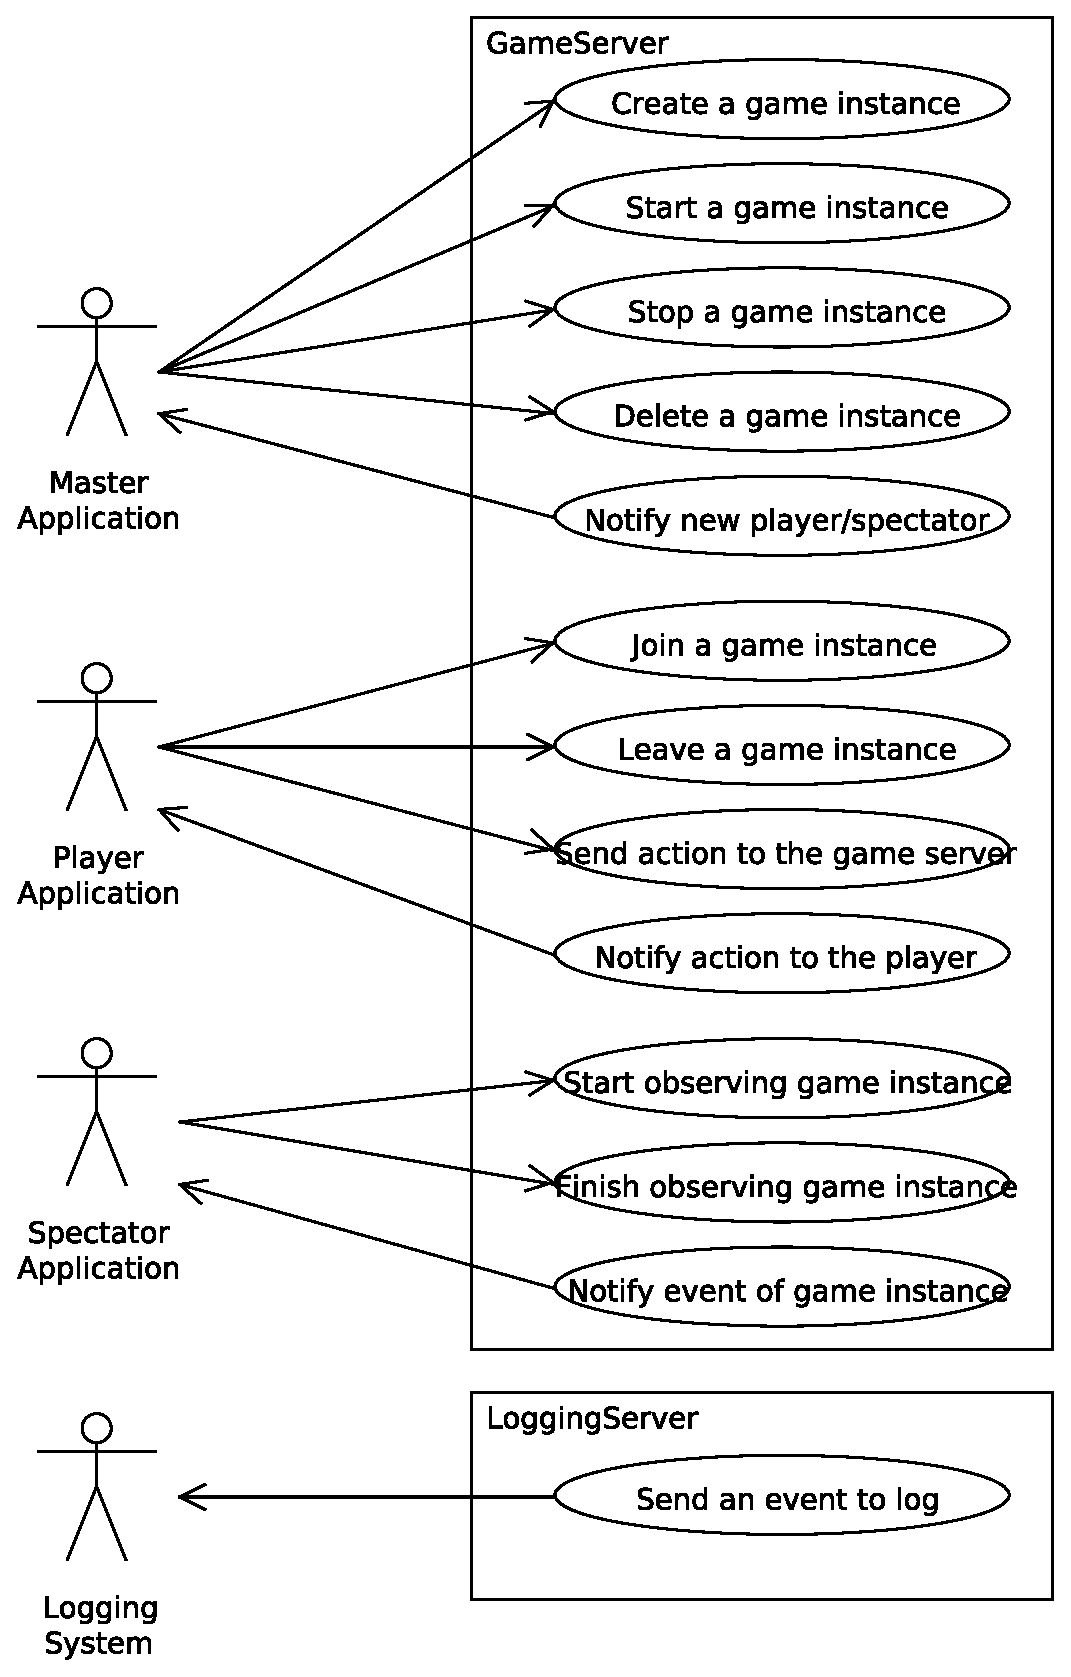
\includegraphics[scale=0.55]{Figures/_integration_use_case_game_server}
\caption{Use case diagram of the subsystem \textsf{Game Server}}
\label{F_integration_use_case_game_server}
\end{center}
\end{figure}

\newpage

The scenarios are modelled into activity diagrams:
\begin{itemize}
\item Figure~\ref{F_integration_activity_create_join} depicts the
  steps of the creation of the game and the game instances, and then
  the steps up to the beginning of the game, that is the period
  during which players and spectators can join the game instance. The
  signals are colored according to the emitter or the receiver:
  magenta is for game masters, cyan is for spectators and yellow is
  for players. Note that the game master that creates a game and the
  game master that creates a game instance may be two different
  participants; in Figure~\ref{F_integration_activity_create_join}, they
  are named $m_1$ and $m_2$, respectively.
\item Figure~\ref{F_integration_activity_be_informed_new_game_instance}
  explains how a player is informed about the list of game instances
  that she can join, and how she ask for joining the chosen game
  instance as player. A similar activity diagram can be drawn to model
  how a spectator chooses the game instance and how she ask for
  joining as a spectator.
\item Figure~\ref{F_integration_activity_leave_game_instance} shows the
  end of a game instance when the game master asks for its closure.
\end{itemize}

\begin{figure}[htbp!]
\begin{center}
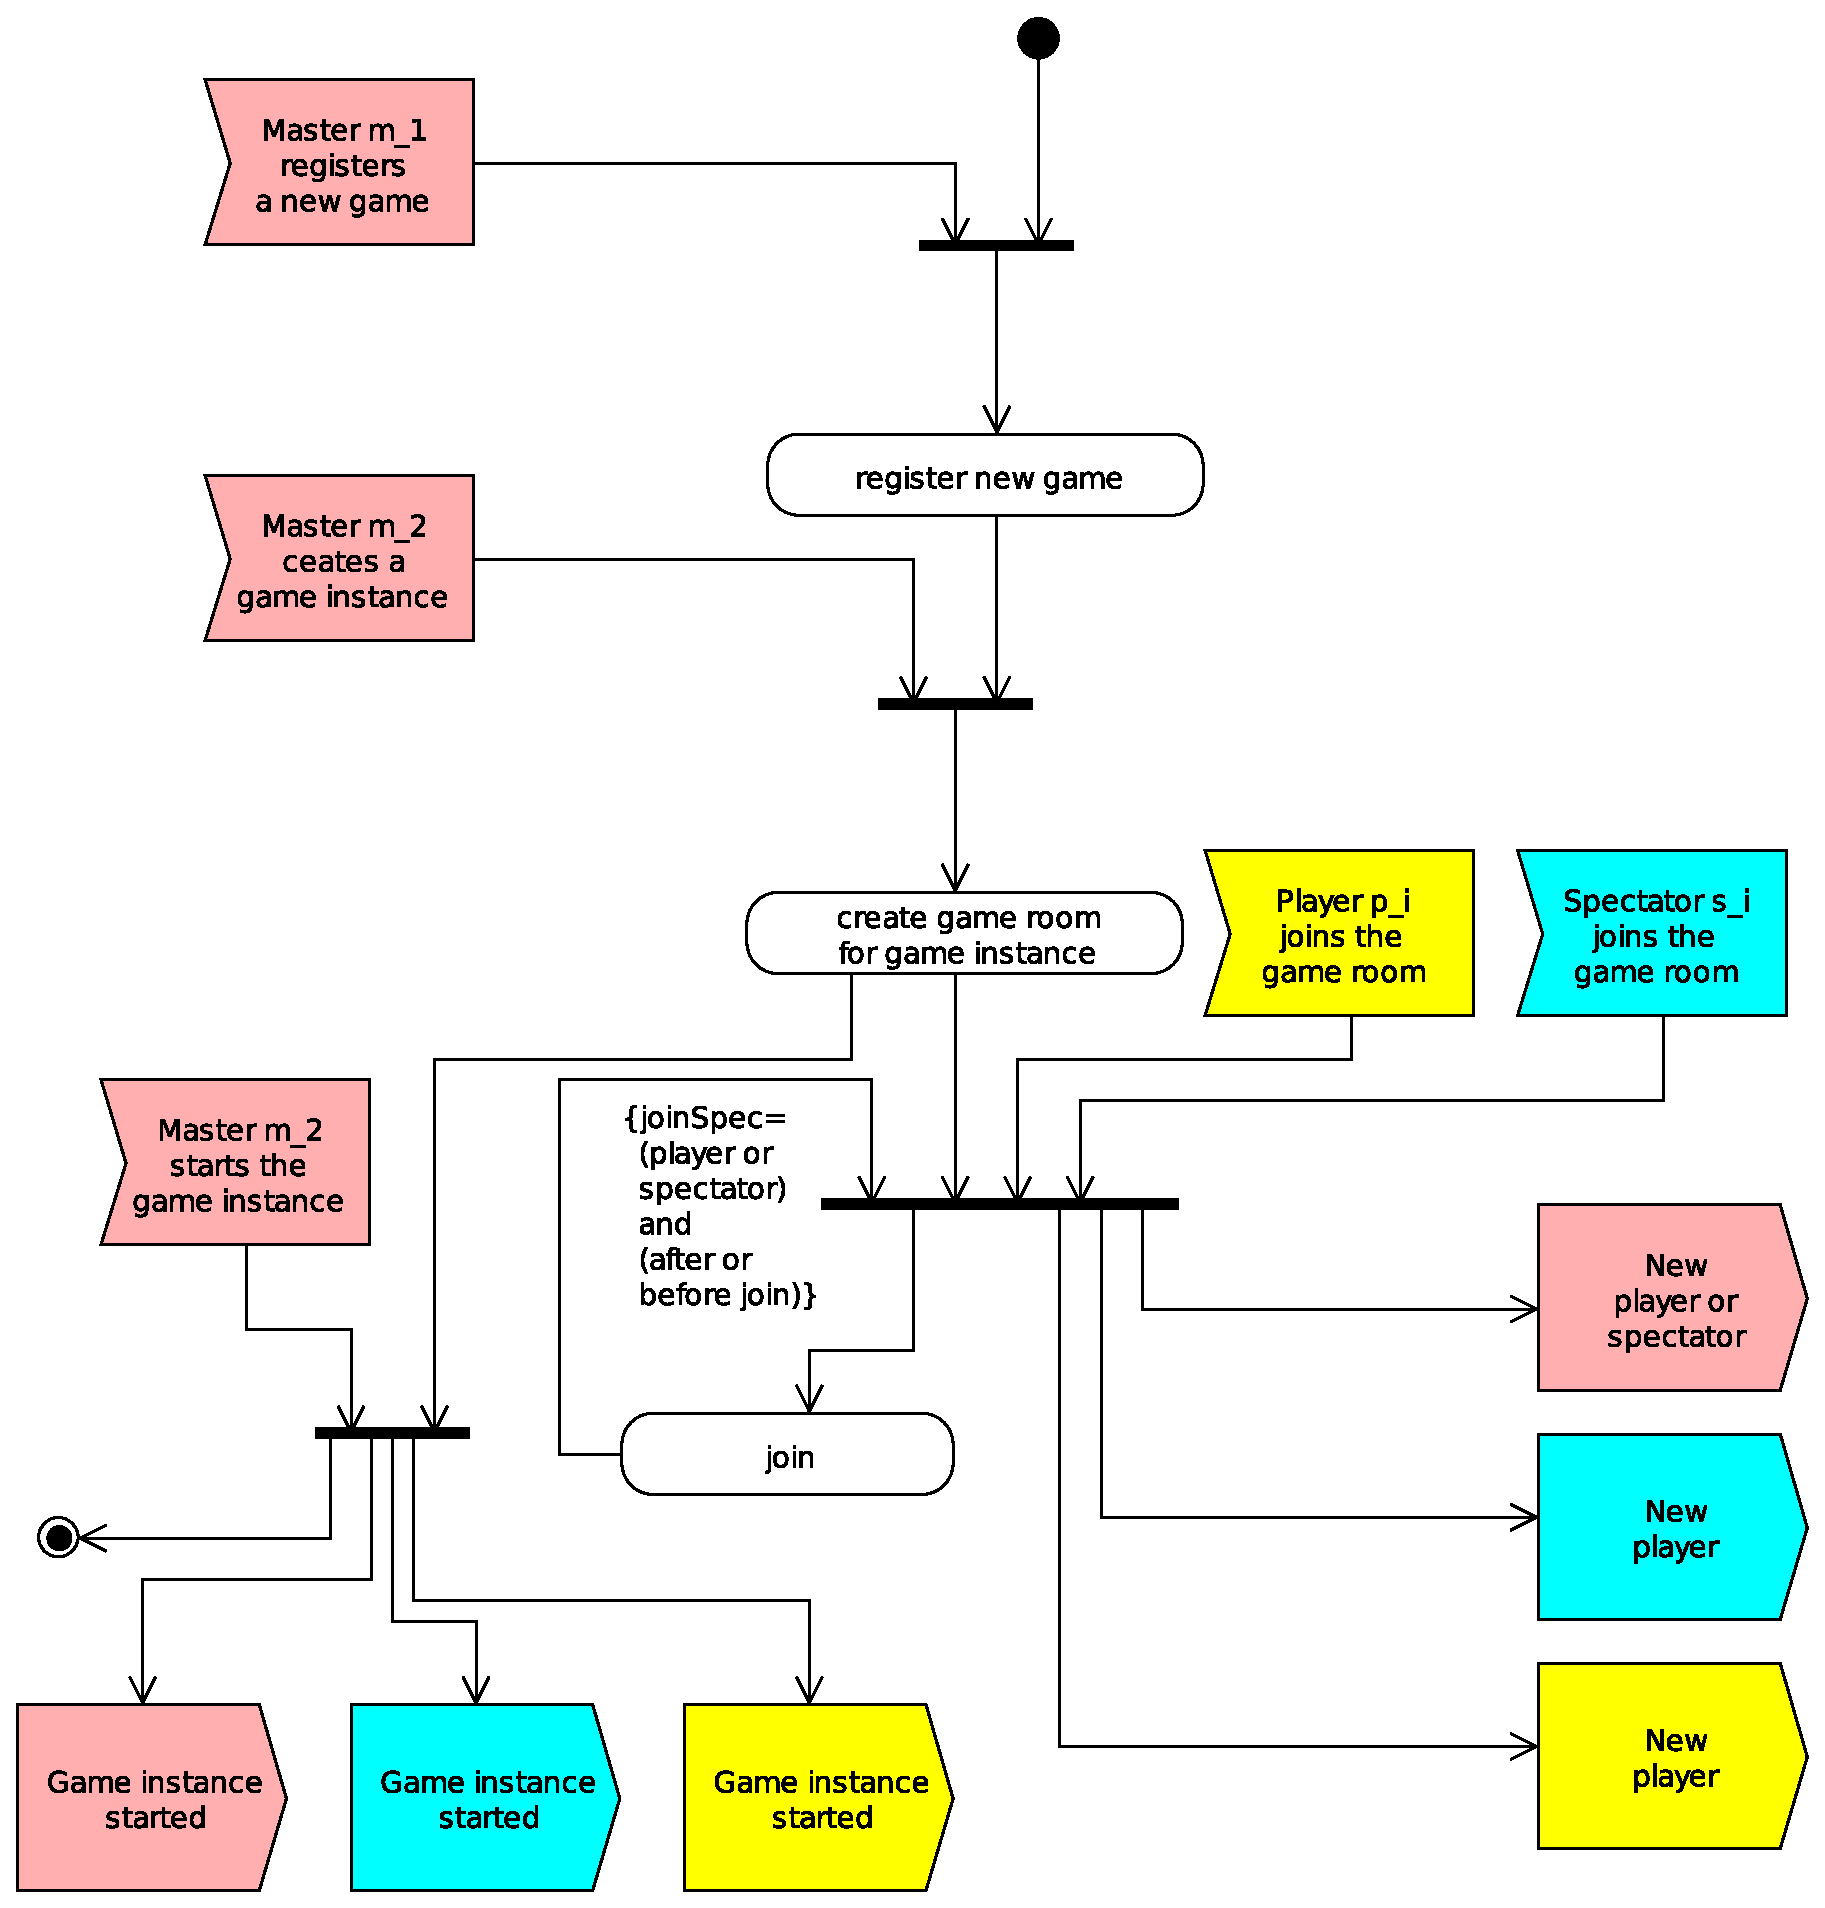
\includegraphics[scale=0.5]{Figures/_integration_activity_create_join_game_instance}
\caption{Activity diagram of the creation of the game and the game
  instance, and of the joining of players and spectators}
\label{F_integration_activity_create_join}
\end{center}
\end{figure}

\begin{figure}[htbp!]
\begin{center}
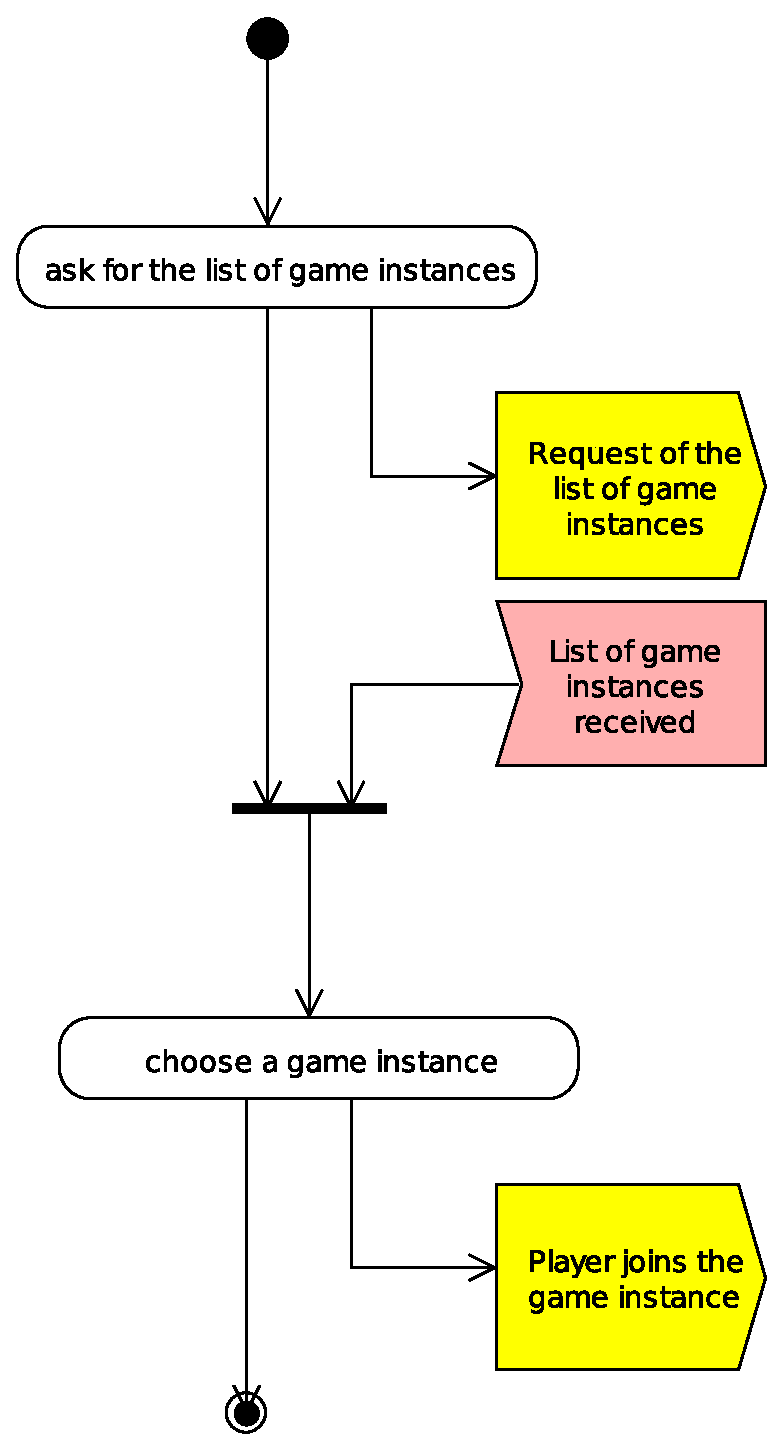
\includegraphics[scale=0.5]{Figures/_integration_activity_be_informed_new_game_instance}
\caption{Activity diagram of how a player is informed about and
  chooses a game instance}
\label{F_integration_activity_be_informed_new_game_instance}
\end{center}
\end{figure}

\begin{figure}[htbp!]
\begin{center}
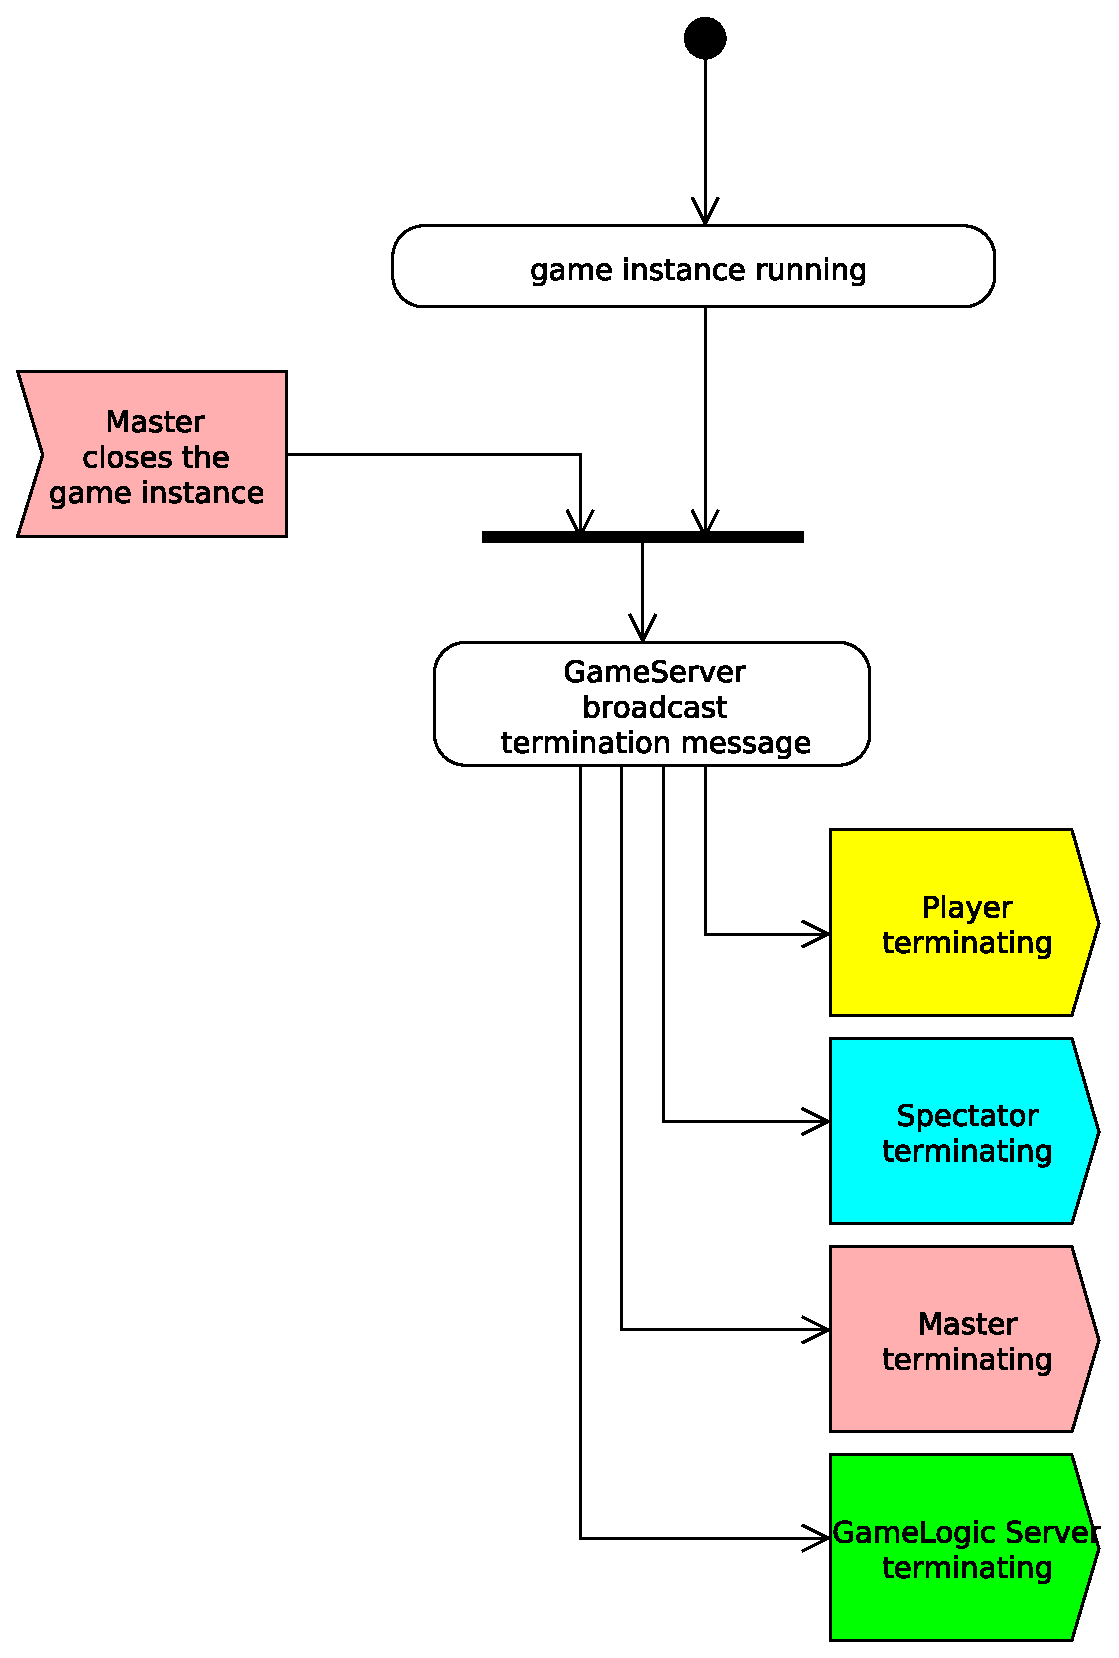
\includegraphics[scale=0.5]{Figures/_integration_activity_leave_game_instance}
\caption{Activity diagram of the end of the game instance}
\label{F_integration_activity_leave_game_instance}
\end{center}
\end{figure}

\newpage

\subsubsection{Business classes}
\label{SSS_integration_analysis}

The static aspects of the analysis of the system is presented in the
class diagram of Figure~\ref{F_integration_class}. This model is very
simple since we have simplified the business concerns in order to
focus on the architectural aspects of the communication part. A \textsf{Game} is
specified by providing a \textsf{name} only. It can be ``played''
several times (possibly in parallel), leading to several
\textsf{Game Instance}s. Each \textsf{Game Instance} is created and
controlled by a \textsf{Participant} called the \textsf{master},
involves several \textsf{Participant}s that are the \textsf{player}s,
and can be followed by other \textsf{Participant}s called the
\textsf{spectator}s. A \textsf{Participant} can take part to several
\textsf{Game Instances} either as \textsf{master}, \textsf{player} or
\textsf{spectator}. A logged message, named a \textsf{Log} for short,
is related to a \textsf{Game Instance} and a \textsf{Participant}. Not
explicitly shown in this diagram, we will allow the logging of purely
``technical messages'' from all the subsystems and that do not concern
a particular \textsf{Game Instance} or a specific
\textsf{Participant}; this is why the multiplicity of the associations
connected to the class \textsf{Log} are ``$0..n$''.

NB~1: In this illustrative application demonstrating the integration of
the different technologies into a consistant communication
architecture, we ignore rights management. In other words, every
participant can be a master and every participant can be a player or a
spectator of every game instance. The \textsf{login} and
\textsf{password} attributes of the class \textsf{Participant} serves
to have access to the communication infrastructure.

NB~2: In this illustrative application, for the sake of simplicity, we
log only events/messages that belong to a game instance.

NB~3: In this illustrative application, no information is stored in a
database, thus there is no database access. This should not be the case
if the application is integrated into the TOTEM \textsf{Django} game
server.

\begin{figure}[htbp!]
\begin{center}
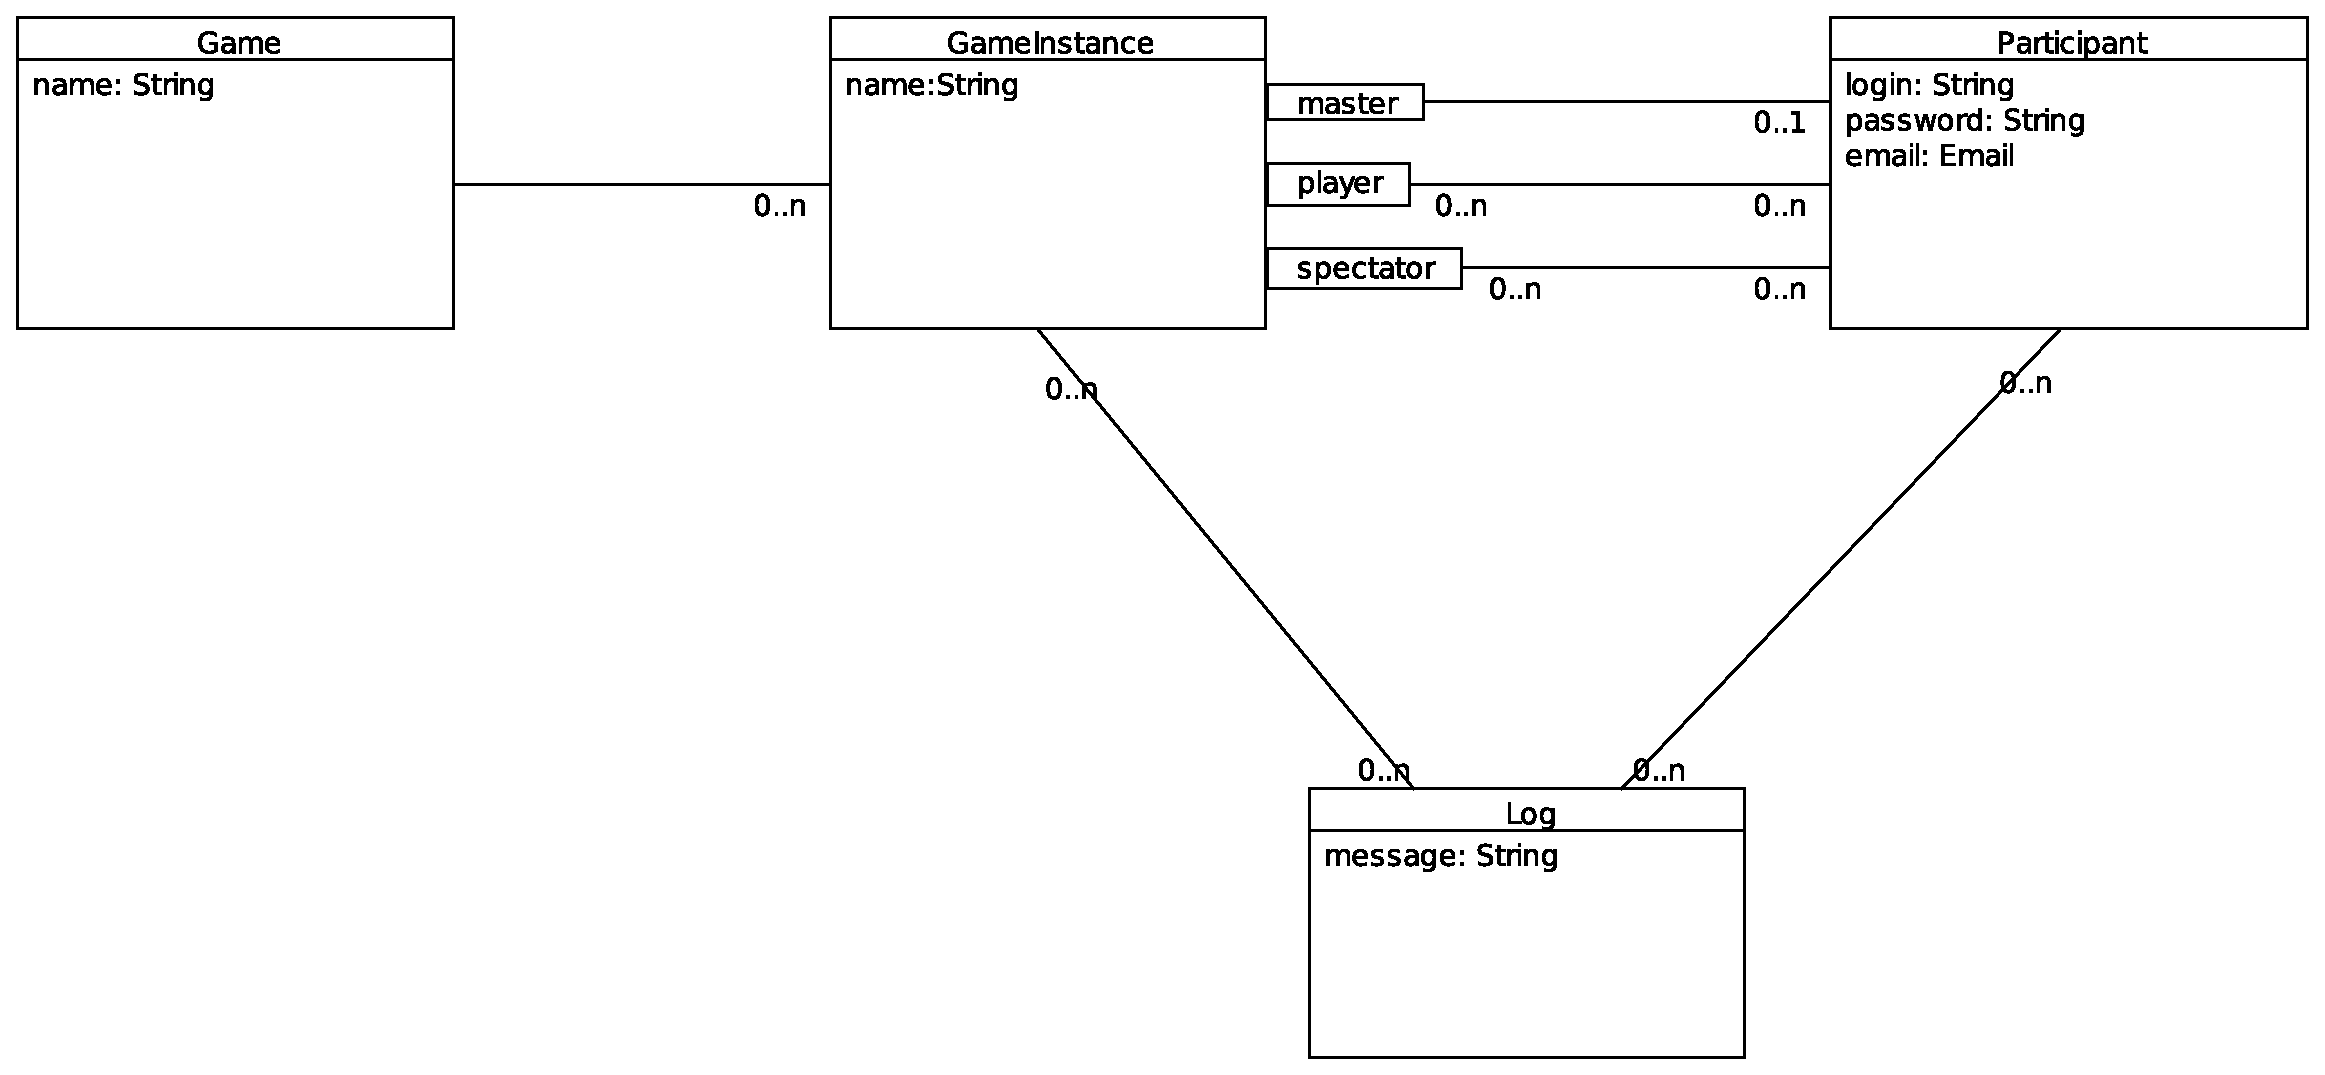
\includegraphics[scale=0.4]{Figures/_integration_class}
\caption{Class diagram of the business concepts used in the subsystems}
\label{F_integration_class}
\end{center}
\end{figure}

\newpage

\subsection{Design of the communication architecture for the game instance}
\label{SS_integration_design}

During a game instance, messages are exchanged through the event-based
system whose configuration is presented in
Figure~\ref{F_architecture_game_instance} (a game instance with a game
logic server, one game master, two players, two spectators, and the
logging mechanism activated). The figure uses the following concepts
from AMQP:
\begin{itemize}
\item The identifier of the game instance serves as the name of the
  virtual host. There is one virtual host per game instance so that
  game executions do not interfer.
\item The first entity in the system is the \textsf{Game Logic
  Server}. It is responsible for creating the topic exchange and the
  queues.
\item Every participant (game master, players, spectators, and logging
  services) has a dedicated queue to receive events.
\item The topic exchange allows filtering with routing keys decomposed
  into four parts: the identifier of the sender (for instance,
  \textsf{p1}), the identifier of the receiver (for instance,
  \textsf{m1}), the kind of action transported in the
  event (for instance, \textsf{join}), and the name of the
  action (for instance, \textsf{joinMaster}).
\item The \textsf{Game Logic Server}, the game master, and the players
  have two bindings: for instance \texttt{*.m1.\#} for receiving
  messages sent only to them, and \texttt{*.all.\#} for receiving
  broadcast messages.
\end{itemize}

The creation and the management of the game instance communication
architecture is described in the following figures:
\begin{itemize}
\item Figure~\ref{F_integration_sequence_game_instance_1} presents the
  sequence diagram of the creation of the game instance and of the
  joining of the \textsf{Master Application} to the game
  instance. The \textsf{Master Application} sends an XMLRPC request to
  the \textsf{Game Server}. The \textsf{Game Server} creates the
  \textsf{Game Logic Server} process. This process is responsible for
  creating the AMQP communication infrastructure and creating the
  thread \textsf{XMLRPC Worker}, which is reponsible for performing
  the join action of the actors. The \textsf{Game Server} and the
  \textsf{Game Logic Server} synchronize using a semaphore so that the
  first join operations are not called before the virtual host and the
  exchange are created.  Figure~\ref{F_architecture_game_instance_1}
  displays the architecture after the creation of the game instance.
  Next, Figure~\ref{F_architecture_game_instance_2} depicts the new
  architecture of the application instance when the \textsf{Master
    Application} has joined the application instance.
\item Figure~\ref{F_integration_sequence_game_instance_2} presents the
  sequence diagram of the joining of a \textsf{Spectator Application}
  to the game instance. The \textsf{Spectator Application} sends an
  XML-RPC request to the \textsf{Game Server} that forwards it to the
  \textsf{XMLRPC Worker} thread of the \textsf{Game Logic
    Server}. Figure~\ref{F_architecture_game_instance_3} depicts the
  new architecture of the application instance when the
  \textsf{Spectator Application} has joined the application instance.
\item Figure~\ref{F_integration_sequence_game_instance_3} presents the
  sequence diagram of the joining a \textsf{Player Application} to the
  game. The \textsf{Player Application} sends an XMLRPC request to the
  \textsf{Game Server} that forwards it to the \textsf{XMLRPC Worker}
  thread of the \textsf{Game Logic
    Server}. Figure~\ref{F_architecture_game_instance_4} depicts the
  new architecture of the application instance when the
  \textsf{Player Application} has joined the application
  instance.
\end{itemize}

NB: in all the models of this section, for the sake of simplicity, we
assume that the actors know their identity and obtain the information
about games and game instances from another means, for instance from
the Web framework. We also assume that they have unique identities
and that their login names do not contain any dot (since the login
names are used for binding and routing keys).

\begin{figure}[htbp!]
\begin{center}
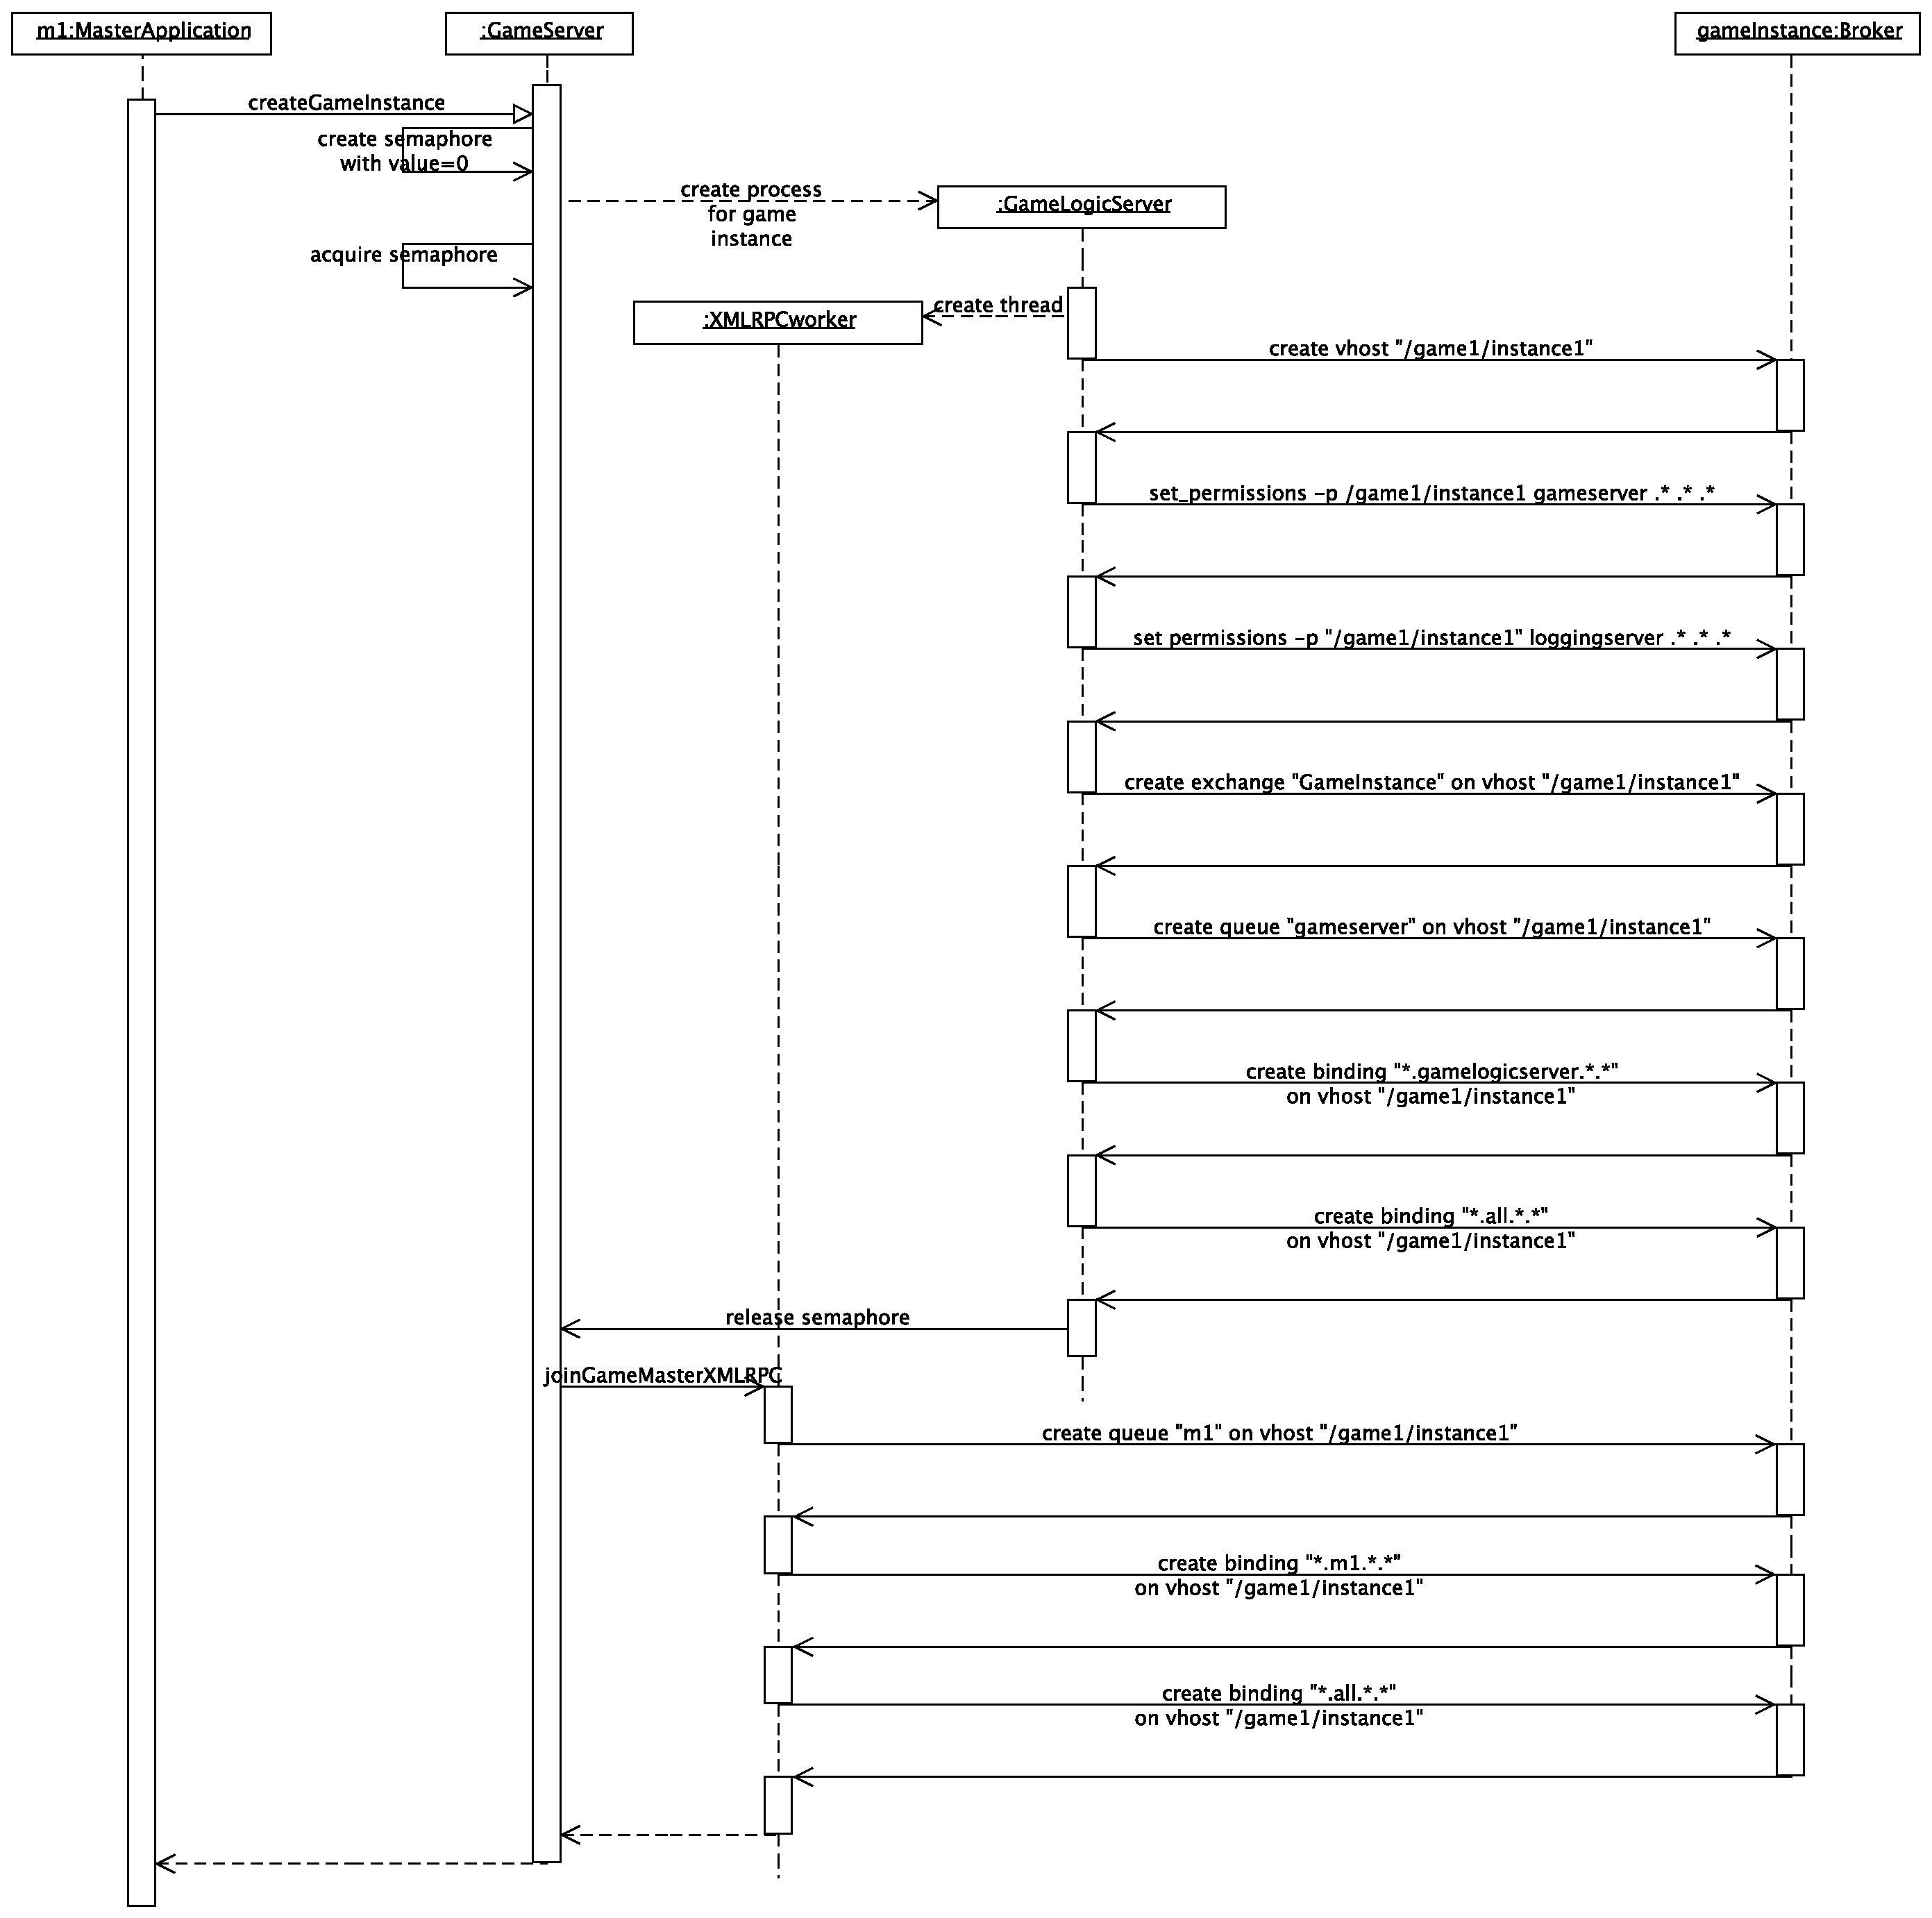
\includegraphics[scale=0.4]{Figures/_integration_sequence_game_instance_1}
\caption{Sequence diagram of the creation of the game instance}
\label{F_integration_sequence_game_instance_1}
\end{center}
\end{figure}

\begin{figure}[htbp!]
\begin{center}
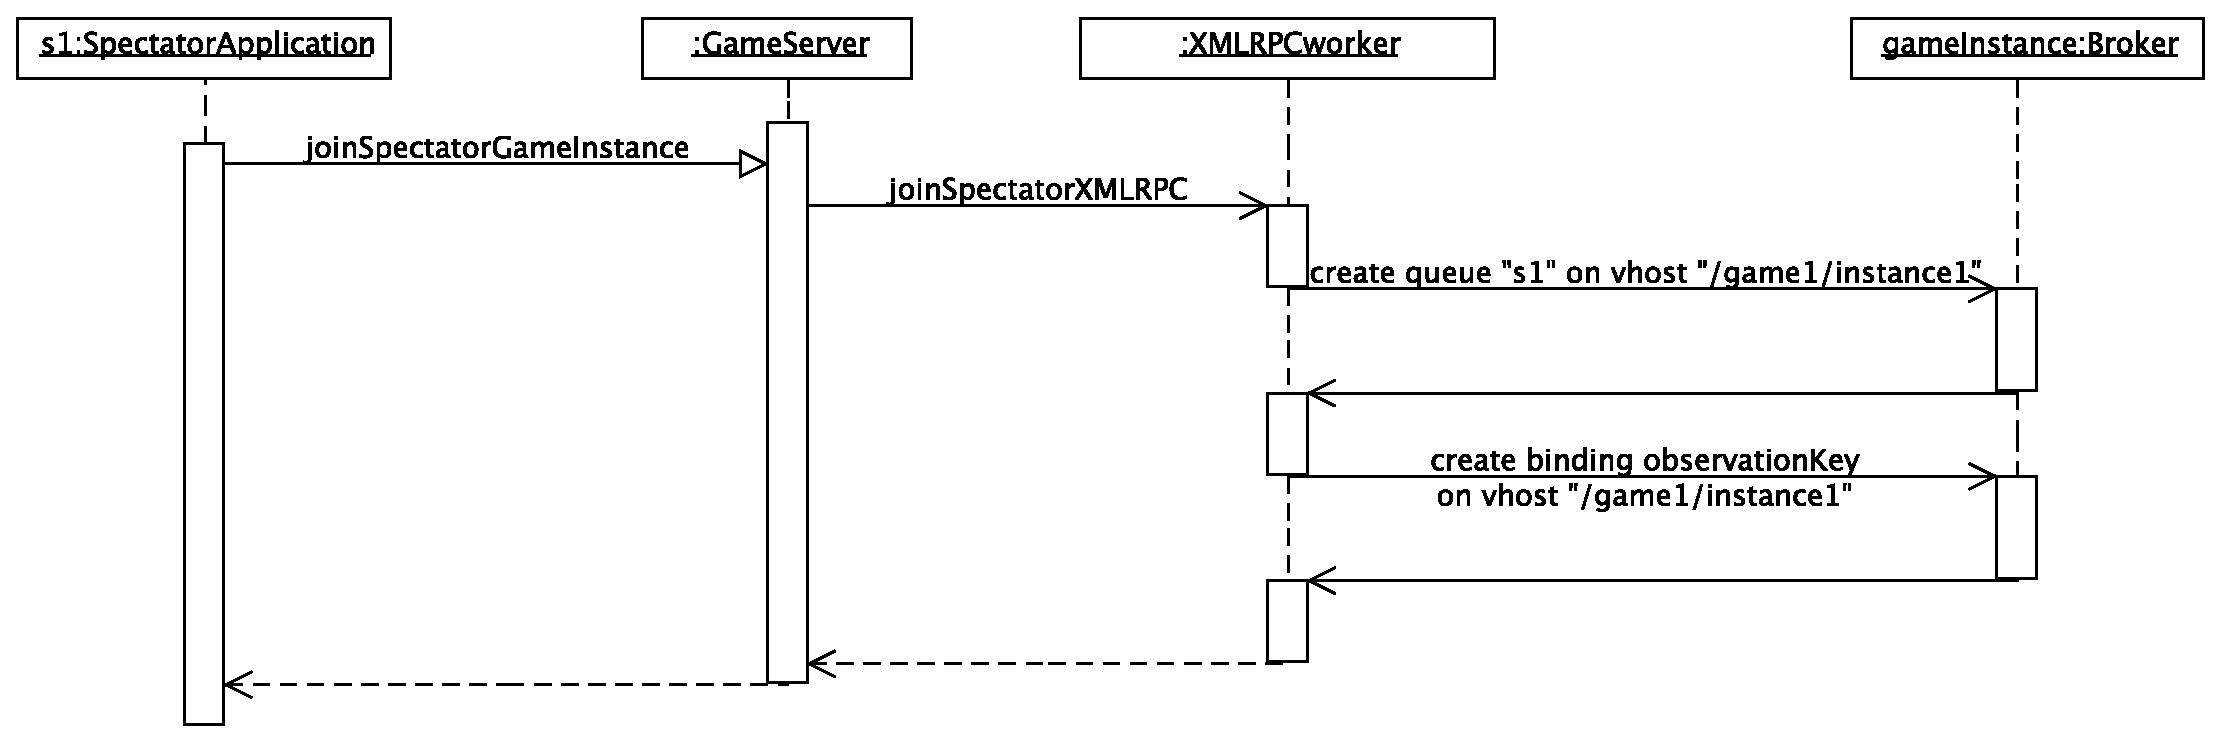
\includegraphics[scale=0.4]{Figures/_integration_sequence_game_instance_2}
\caption{Sequence diagram of the joining of the \textsf{Spectator
    Application} to the game instance}
\label{F_integration_sequence_game_instance_2}
\end{center}
\end{figure}

\begin{figure}[htbp!]
\begin{center}
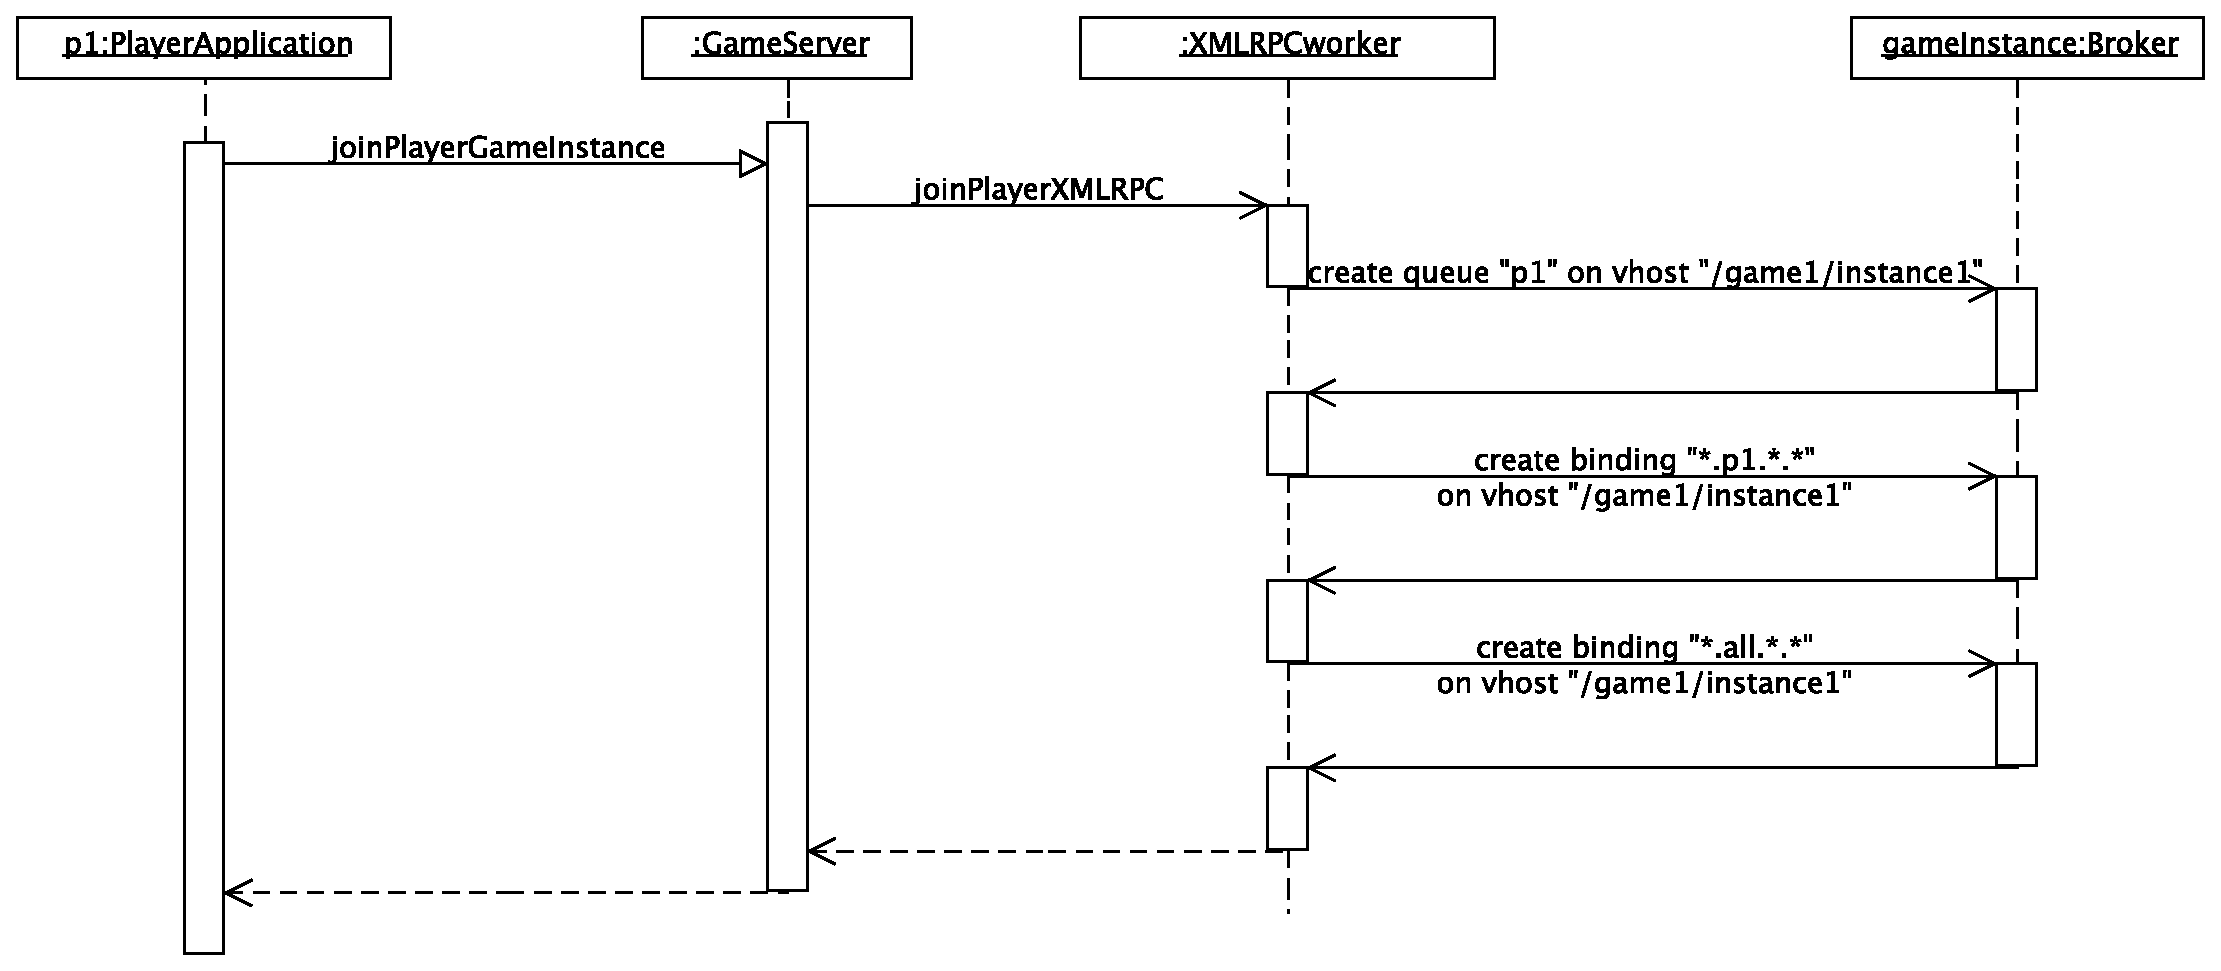
\includegraphics[scale=0.4]{Figures/_integration_sequence_game_instance_3}
\caption{Sequence diagram of the joining of a \textsf{Player
    Application} to the game instance}
\label{F_integration_sequence_game_instance_3}
\end{center}
\end{figure}

\begin{figure}[htbp!]
\begin{center}
\includegraphics[scale=0.6,angle=90]{Figures/architecture_game_instance_1}
\caption{Architecture of the subsystem for the game instance
  (at creation time)}
\label{F_architecture_game_instance_1}
\end{center}
\end{figure}

\begin{figure}[htbp!]
\begin{center}
\includegraphics[scale=0.6,angle=90]{Figures/architecture_game_instance_2}
\caption{Architecture of the subsystem for the game instance after
  the game master has joined the game instance}
\label{F_architecture_game_instance_2}
\end{center}
\end{figure}

\begin{figure}[htbp!]
\begin{center}
\includegraphics[scale=0.6,angle=90]{Figures/architecture_game_instance_3}
\caption{Architecture of the subsystem for the game instance after a
  spectator has joined the game instance}
\label{F_architecture_game_instance_3}
\end{center}
\end{figure}

\begin{figure}[htbp!]
\begin{center}
\includegraphics[scale=0.6,angle=90]{Figures/architecture_game_instance_4}
\caption{Architecture of the subsystem for the game instance after a
  player has joined the game instance}
\label{F_architecture_game_instance_4}
\end{center}
\end{figure}

\newpage

\subsection{Implementation and execution}
\label{SS_integration_implementation}

The implementation of the example application is available in the
Subversion repository of the TOTEM Redmine in the directory
structure \begin{small}\texttt{TOTEM.CommunicationMiddleware/\-Sources/\-Integration\-Example\-Application}\end{small}.

The prerequisites are listed in the file \texttt{readme.txt}:
\begin{itemize}
\item Software to install and to configure:
\begin{itemize}
\item For the server side:
\begin{itemize}
\item \texttt{Erlang} version $\geq$ R13B03,
\item \texttt{RabbitMQ Server} version $\geq$ 2.7.1,
\item \texttt{Pika} version $\geq$ 0.9.5.
\end{itemize}
\item For Android clients:
\begin{itemize}
\item \texttt{Android SDK API level} $\geq$ 7.
\end{itemize}
\item For Java clients:
\begin{itemize}
\item \texttt{Maven} version $\geq$ 2.2.1,
\item \texttt{Java JRE} $\geq$ 1.5.
\end{itemize}
\item For JavaScript clients:
\begin{itemize}
\item \texttt{Node.js} $\geq$ 0.4.10
\end{itemize}
\end{itemize}

\item Subsystems of the example application to ``install'':
\begin{itemize}
\item \textsf{GameServer}: a Python project using XML-RPC
  communication to create and control the game logic servers. This is
  the project that should be integrated into the Web Framework.
\item \textsf{GameLogicServer}: a Python project using AMQP
  communication to control the execution of the game instance. This is
  where game developers put the logic of the server of the game.
\item \textsf{MasterApplication} for Java J2SE: a Maven project using
  the \textsf{RabbitMQ} Java Client (for J2SE\footnote{As demonstrated
    with the examples written using the \textsf{RabbitMQ} and
    \textsf{XML-RPC} Java Client for Android, there is no significant
    differences between a J2SE client application and its Android
    version.}). The directory contains also the shell script
  \texttt{run.sh} to launch this subsystem.
\item \textsf{PlayerMasterAndroid} for Android device: This is the
  Eclipse Android project that can be imported into Eclipse for
  compiling and generating Android artefacts. When launching the
  application, it is possible to chose between creating or joining a
  game instance.
\item \textsf{MasterApplicationJavascript}: This is the Web application
  for the master. Before launching this application in a Web browser, 
  you have to start NodeJsProxy first, as mentionned in 
  NodeJsProxy/readme.txt.
\item \textsf{SpectatorApplication} for Java J2SE: a Maven project
  using the \texttt{RabbitMQ} Java Client (for J2SE). The directory
  contains also the shell script \textsf{run.sh} to launch this
  subsystem.
\item \textsf{SpectatorApplicationJavascript}: This is the Web application
  for spectators. Before launching this application in a Web browser, 
  you have to start NodeJsProxy first, as mentionned in 
  NodeJsProxy/readme.txt.
\item \textsf{NodeJsProxy}: This is the proxy used both by Master and 
  Spectator applications in JavaScript to log-in and to 
  establish their AMQP connections with the  RabbitMQ broker.
\item \textsf{PlayerApplication} for Java J2SE: a Maven project using
  the \texttt{RabbitMQ} Java Client (for J2SE). The directory contains
  also the shell script \textsf{run.sh} to launch this subsystem.
\end{itemize}
\end{itemize}

\textbf{NB:} All the projects / directories mentionned in the previous
list are complemented with \texttt{readme.txt} files. Please refer to
the \texttt{readme.txt} file at the root directory for installation
and execution instructions.
\bigskip 
\newline 
\important{Do not forget to adapt the \textsf{RabbitMQ} and
  \textsf{XML-RPC} configuration properties such as the IP addresses
  of the \textsf{RabbitMQ} broker and \textsf{XML-RPC} servers to your
  execution environment. Here are the files you need to modify:
\begin{itemize}
\item For the Android Application: \texttt{\-PlayerMasterAndroid/\-res/\-raw/\-rabbitmq.properties} and \texttt{\-PlayerMasterAndroid/\-res/\-raw/\-xmlrpc.properties}
\item For Java J2SE Applications: \texttt{*\-src/\-main/\-ressources/\-rabbitmq.properties} and \texttt{*\-src/\-main/\-resources/\-xmlrpc.properties}
\item For Javascript Applications: \texttt{\-NodeJsProxy/\-resources/\-rabbitmq.properties} and \texttt{\-NodeJsProxy/\-resources/\-xmlrpc.properties}
\end{itemize}} 
\newline
\newline
To launch the example application on a Unix-like operating
system with the Java J2SE
clients, execute the script \textsf{./run.sh}. This script launches
all the subsystems in sequence with some of the processes in
background mode. The sequence starts with the stopping and
initialisation of the \textsf{RabbitMQ} broker, so that no
interference can happen with another running application. 
\newline
\newline
Other scripts exist:
\begin{itemize}
\item for Unix-like operating systems:
\begin{itemize}
\item \textsf{run\_with\_android\_phones.sh}: the same as \textsf{run.sh}
  one but for running on Android phones.
\item \textsf{run\_with\_master\_and\_spectators\_javascript.sh}: the 
same as \textsf{run.sh} but using Master and Spectator Web applications.
Of course, you can also launch additional Java or Android players, and 
Java or Android spectators.
\item \textsf{termination.sh}: to send a terminate message to all the
  clients of all the available game instances. It terminates all the
  game instances and the whole server side.
\end{itemize}
\item for Windows operating systems:
\begin{itemize}
\item \textsf{run\_with\_android\_phones.bat}: the same as \textsf{run\_with\_android\_phones.sh}.
\item \textsf{termination.bat}: the same as \textsf{termination.sh}.
\end{itemize}
\end{itemize}

To run all these scripts, follow the instructions.

\endinput

\newpage

\appendix
\addcontentsline{toc}{section}{Appendix}

\newpage

% TCM: TOTEM Communication Middleware
% Copyright: Copyright (C) 2009-2012
% Contact: denis.conan@telecom-sudparis.eu, michel.simatic@telecom-sudparis.eu
% Permission is granted to copy, distribute and/or modify this document
% under the terms of the GNU Free Documentation License, Version 1.3
% or any later version published by the Free Software Foundation;
% with no Invariant Sections, no Front-Cover Texts, and no Back-Cover Texts.
% A copy of the license is included in the section entitled "GNU
% Free Documentation License".

\section{Installation of RabbitMQ}
\label{S_installation_rabbitmq_local}

In this section, we provide the procedure for installing
\textsf{RabbitMQ}: the broker, the Java client for Android phones, the
Python client for the web framework, and the JavaScript client for the
Browser. Similar instructions are included in a separate section,
namely Section~\ref{SS_ec2_configure_instance}, for installing
\textsf{RabbitMQ} on Amazon EC2 cloud.

\subsection{RabbitMQ broker on desktop computers}

In this section, we install the software from a regular archive so
that we will execute \textsf{RabbitMQ} broker as a non-\texttt{root}
user. The configuration of the environment
variables \begin{small}\texttt{RABBITMQ\_MNESIA\_BASE}\end{small}
and \begin{small}\texttt{RABBITMQ\_LOG\_BASE}\end{small} is important
to allow executing the broker as a non-\texttt{root} user. This is
done as follows.
\begin{enumerate}
\item The instructions we provide are extracted from the ``install''
  Web page at this
  URL: \begin{small}\texttt{http://www.rabbitmq.com/\-install.html}\end{small}. Refer to this Web page when necessary.
\begin{itemize}
\item At first, install Erlang and Python 2.6:
\begin{itemize}
\item On GNU/Linux, Debian distribution, check the versions that are
  installed, executing the following commands:
\begin{shellcmd}
\$ erl
Erlang R13B03 (erts-5.7.4) [source] [smp:2:2] [rq:2] [async-threads:0] [hipe] [kernel-poll:false]

Eshell V5.7.4  (abort with ^G)
...
\$ python --version
Python 2.6.6
\end{shellcmd}
\item Or execute the following commands as the user \textsf{root} or
  as a \textsf{sudouser}:
\begin{shellcmd}
apt-get install erlang
apt-get install python
\end{shellcmd}
\end{itemize}
\item Next, install \textsf{RabbitMQ} version~2.7.1 from the ``Package
  for generic Unix systems'' (file
  \textsf{rabbitmq-server-generic-unix-2.7.1.tar.gz}) or from the
  ``Windows Bundle'' (file
  \textsf{rabbitmq-server-windows-2.7.1.zip}). In the following, adapt
  the commands if you are running a Windows operationg system (cf.~the
  Web
  page \begin{small}\texttt{http://\-www.\-rabbitmq.\-com/\-install.\-html\#\-windows}\end{small}).
\begin{itemize}
\item On GNU/Linux, Debian distribution, execute the following commands:
\begin{shellcmd}
wget http://www.rabbitmq.com/releases/rabbitmq-server/ \textbackslash
     v2.7.1/rabbitmq-server-generic-unix-2.7.1.tar.gz
tar xfz rabbitmq-server-generic-unix-2.7.1.tar.gz
\end{shellcmd}
\end{itemize}
\end{itemize}
On Unix-like operating systems, the broker of \textsf{RabbitMQ},
called the server in \textsf{RabbitMQ} terminology, is now installed
in the directory
\textsf{\textsc{\$\{yourdirectory\}}/rabbitmq\_server-2.7.1}.  The
commands of \textsf{RabbitMQ} (\textsf{rabbitmq-server} to launch the
broker and \textsf{rabbitmqctl} to control the broker) are available
in the directory
\textsf{\textsc{\$\{yourdirectory\}}/rabbitmq\_server-2.7.1/sbin}.

\item

\begin{enumerate}
\item On Unix-like operating systems, in order to add the
  \textsf{RabbitMQ} commands to the shell path, and to configure the
  location of the database and the log files, add the following
  commands to the shell script that is executed when opening a shell
  connection, for instance in the file \textsf{\string~/.bashrc}:
\begin{shellcmd}
PATH=\${PATH}:\textsc{\$\{yourdirectory\}}/rabbitmq\_server-2.7.1/sbin
export RABBITMQ\_MNESIA\_BASE=\textsc{\$\{yourdirectory\}}/rabbitmq\_server-2.7.1/mnesia
export RABBITMQ\_LOG\_BASE=\textsc{\$\{yourdirectory\}}/rabbitmq\_server-2.7.1/log
\end{shellcmd}
Note that we assume that you are now going to create the directories
\textsf{\textsc{\$\{yourdirectory\}}/rabbitmq\_server-2.7.1/mnesia}
and \textsf{\textsc{\$\{yourdirectory\}}/rabbitmq\_server-2.7.1/log}.

\item On Windows systems, follow the instructions in \begin{small}\texttt{http://\-www.\-rabbitmq.\-com/\-install.\-html\#\-windows}\end{small}, that is:
\begin{itemize}
\item Set \textsf{\textsc{erlang\_home}} environment variable to where
  you actually put your Erlang installation,
  e.g. \textsf{C:\textbackslash{}Program
    Files\textbackslash{}erl5.7.4} (full path). The \textsf{RabbitMQ}
  batch files expect to execute
  \textsf{\textsc{\%erlang\_home}\%\textbackslash{}bin\textbackslash{}erl.exe}.
\item Create a system environment variable
  (e.g. \textsf{\textsc{rabbitmq\_server}}) for
  \textsf{C:\textbackslash{}Program
    Files\textbackslash{}RabbitMQ\textbackslash{}rabbitmq\_server-2.7.1}.
  Adjust this if you put \textsf{rabbitmq\_server-2.7.1} elsewhere.
\item Append the literal string
  \texttt{;\textsc{\%rabbitmq\_server}\%\textbackslash{}sbin} to your
  system path (as known as \texttt{\%PATH\%}).
\end{itemize}
Note: On Windows systems, it is not necessary to create and set the
variables \texttt{\textsc{rabbitmq\_mnesia\_base}} and
\texttt{\textsc{rabbitmq\_log\_base}}.
\end{enumerate}

\item
On Unix-like and Windows operating systems, your \textsf{RabbitMQ}
installation can be tested by launching the broker as follows:
\begin{shellcmd}
\$ rabbitmq-server -detached \# execute in the background
Activating RabbitMQ plugins ...
0 plugins activated:
\$ rabbitmqctl status
Status of node rabbit@rabbit ...
[{running\_applications,[{rabbit,"RabbitMQ","2.7.1"},
                        {mnesia,"MNESIA  CXC 138 12","4.4.14"},
                        {os\_mon,"CPO  CXC 138 46","2.2.5"},
                        {sasl,"SASL  CXC 138 11","2.1.9.2"},
                        {stdlib,"ERTS  CXC 138 10","1.17"},
                        {kernel,"ERTS  CXC 138 10","2.14"}]},
 {nodes,[{disc,[rabbit@rabbit]}]},
 {running\_nodes,[rabbit@rabbit]}]
...done.
\$ rabbitmqctl stop
Stopping and halting node rabbit@rabbit ...
...done.
\$ rabbitmqctl status
Status of node rabbit@rabbit ...
Error: unable to connect to node rabbit@rabbit: nodedown
diagnostics:
- nodes and their ports on rabbit: [{rabbitmqctl2776,45667}]
- current node: rabbitmqctl2776@rabbit
- current node home dir: /home/bitnami
- current node cookie hash: 58UmUjslvHMdJuJyRDcEag==
\end{shellcmd}
\end{enumerate}

\subsection{RabbitMQ producers and consumers on J2SE applications,
  dedicated RabbitMQ Java client library}
\label{S_rabbitmq_android_phones}

The library for Java producers and consumers of
\textsf{RabbitMQ}, called clients in \textsf{RabbitMQ} terminology, is 
downloaded using Maven. To test the library with your environment, you can do the following:
\begin{itemize}
\item At first, install Sun JDK 1.6 and Maven 2:
\begin{itemize}
\item On GNU/Linux, Debian distribution, check the versions that are
  installed, executing the following commands:
\begin{shellcmd}
\$ java -version
java version "1.6.0_24"
...
\$ javac -version
javac 1.6.0_24
\$ mvn -version
Apache Maven 2.2.1 (rdebian-4)
Java version: 1.6.0_24
Java home: /usr/lib/jvm/java-6-sun-1.6.0.24/jre
\end{shellcmd}
\item Or execute the following commands as the user \textsf{root} or
  as a \textsf{sudoer}:
\begin{shellcmd}
apt-get install sun-java6-jdk
apt-get install maven2
\end{shellcmd}
\end{itemize}
\item Download the directory  \begin{small}\texttt{Totem.CommunicationMiddleware/Sources/TutorialExamples/J2SE/Step1}\end{small}
from the TOTEM Redmine Subversion repository.
\item Launch the RabbitMQ broker, and the J2SE consumers and producers using the script \textsf{run.sh}.
\end{itemize}

\subsection{RabbitMQ producers and consumers on desktop computers,
  Python RabbitMQ client library named Pika}

To limit the number of commands requiring \texttt{root} privileges, we
propose to not install the Python packages using the \texttt{pip} or
\texttt{easy\_install} utility tools. But, of course, you can prefer
performing this installation differently using Python utility
tools. In addition, we only provide the commands for Unix-like
operating systems.

\begin{enumerate}
\item Install the software Pika, version 0.9.5 by executing the following commands
\begin{shellcmd}
\$ cd \textsc{\$\{yourdirectory\}}
\$ wget http://pypi.python.org/packages/source/p/pika/pika-0.9.5.tar.gz
\$ tar xfz pika-0.9.5.tar.gz
\end{shellcmd}
The Python packages Pika is installed in the directory
\textsf{\textsc{\$\{yourdirectory\}}/pika-v0.9.5}.  Insert this
package in the path of Python by adding the directories in the shell
variable \textsf{PYTHONPATH}:
\begin{shellcmd}
export PYTHONPATH=\$PYTHONPATH:\textsc{\$\{yourdirectory\}}/pika-v0.9.5
\end{shellcmd}
\item Check that Pika is correctly installed by trying the following
  Python commands that demonstrate that the Pika package can be
  imported in a Python script:
\begin{shellcmd}
\$ python
Python 2.6.5 (r265:79063, Apr 16 2010, 13:09:56) 
[GCC 4.4.3] on linux2
Type "help", "copyright", "credits" or "license" for more information.
>>> import pika
>>> quit()
\end{shellcmd}
\end{enumerate}

To test the library with your environment, you can do the following:
\begin{itemize}
\item Download the
  directory \begin{small}\texttt{Totem.CommunicationMiddleware/Sources/TutorialExamples/Pika/Step5}\end{small}
  from the TOTEM Redmine Subversion repository.
\item Start the \textsf{RabbitMQ} server with the following command:
\begin{shellcmd}
\$ rabbitmq-server
Activating RabbitMQ plugins ...
0 plugins activated:
...
\end{shellcmd}
\item Check that there is no exhange named \textsf{topic\_logs} by
  executing the following commands:
\begin{shellcmd}
\$ rabbitmqctl list\_exchanges
Listing exchanges ...
amq.direct	direct
amq.topic	topic
amq.rabbitmq.log	topic
amq.fanout	fanout
amq.headers	headers
	direct
amq.match	headers
...done.
\$ rabbitmqctl list\_bindings
Listing bindings ...
...done.
\end{shellcmd}
\item Launch the consumers and the producers using the script
  \texttt{run.sh}.
\end{itemize}


\subsection{RabbitMQ JavaScript producers and consumers using
JavaScript AMQP library}
\label{javascript-node.js}

The library for Javascript AMQP producers and consumers works with
\textsf{Node.js}, which is an event-driven I/O server-side JavaScript
environment. Here follows an installation procedure for Unix-like
operating systems which should be performed on the server side:

\begin{enumerate}
\item Install \textsf{Node.js}:

\begin{itemize}
\item The prerequisites to build \textsf{Node.js} from source are:
\begin{itemize}
\item \textsf{python}: version~2.4 or higher. The build tools distributed with 
\textsf{Node.js} run on python.
\item \textsf{libssl-dev}: If you plan to use SSL/TLS encryption in
  your networking, you need this library. \texttt{libssl} is the
  library used in the \texttt{openssl} tool.
\end{itemize}
\item To download and build \textsf{Node.js}, version~0.4.10 execute the 
following commands:

\begin{shellcmd}
\$ mkdir \textasciitilde/node.js
\$ cd 	\textasciitilde/node.js
\$ wget http://nodejs.org/dist/node-v0.4.10.tar.gz
\$ tar xfz node-v0.4.10.tar.gz
\$ rm node-v0.4.10.tar.gz
\$ cd node-v0.4.10
\$ ./configure --prefix=\$HOME/node.js/node-v0.4.10
\$ make
\$ make install
\$ echo "export PATH=\$HOME/node.js/node-v0.4.10/bin:\$PATH" >> \textasciitilde/.bashrc
\$ echo "export NODE_PATH=\$HOME/node.js/node-v0.4.10:\$HOME/\textbackslash
  node.js/node-v0.4.10/lib/node_modules" >> \textasciitilde/.bashrc
\$ source \textasciitilde/.bashrc
\end{shellcmd}
\item Check that \textsf{node.js} is properly installed by trying the following
command:
\begin{shellcmd}
\$ node -v
v0.4.10
\end{shellcmd}
\end{itemize}

\item Install \textsf{npm}, the package manager for installing additional 
\textsf{Node.js} libraries:
\begin{itemize}
\item If the \textsf{curl} command is not present, you should first install it:
\begin{shellcmd}
\$ sudo apt-get install curl
\end{shellcmd}
\item Then, install \textsf{npm}:
\begin{shellcmd}
\$ curl http://npmjs.org/install.sh | sh
\end{shellcmd}
\end{itemize}

\item Install \textsf{node-amqp} \textit{(version 0.1.0)}, an AMQP client for \textsf{Node.js} by 
executing the following command:
\begin{shellcmd}
\$ npm install -g amqp@0.1.0
\end{shellcmd}

\item Install \textsf{node-mxlrpc}, an XMLRPC client for \textsf{Node.js} by 
executing the following command:
\begin{shellcmd}
\$ npm install -g xmlrpc
\end{shellcmd}
\end{enumerate}

To test the AMQP library with your environment, you can do the following:
\begin{itemize}
\item Download the
  directory \begin{small}\texttt{Totem.CommunicationMiddleware/Sources/TutorialExamples/Javascript}\end{small}
  from the TOTEM Redmine Subversion repository.
\item Enter the \begin{small}\texttt{Step1}\end{small} folder, and launch 
the consumer and the producer using \texttt{run.sh}.\bigskip 
\item At the end of the execution of the script \texttt{run.sh} ,
  check that the output looks like this one:
\begin{shellcmd}
[...]
Starting node rabbit@rabbit ...
...done.
Producer connected to broker.
queue declared.
message published.
Listing queues ...
hello_queue	false	false
...done.
Consumer connected to broker.
Message received: Hello world!
Stopping and halting node rabbit@rabbit ...
...done.
END OF HELLOWORLD TUTORIAL TEST
\end{shellcmd}
\note{Warning:}{ Using the script to launch the consumer and the
  producer will delete every queues and exchanges located on your
  broker. If you don't want to do so, please refer to the
  \texttt{readme.txt} file.}
\end{itemize}

\endinput


\newpage

% TCM: TOTEM Communication Middleware
% Copyright: Copyright (C) 2009-2012
% Contact: denis.conan@telecom-sudparis.eu, michel.simatic@telecom-sudparis.eu
% Permission is granted to copy, distribute and/or modify this document
% under the terms of the GNU Free Documentation License, Version 1.3
% or any later version published by the Free Software Foundation;
% with no Invariant Sections, no Front-Cover Texts, and no Back-Cover Texts.
% A copy of the license is included in the section entitled "GNU
% Free Documentation License".

\section{Installation of RabbitMQ and Pika on Amazon EC2}
\label{S_installation_rabbitmq_ec2}

 \note{Important note:}{This appendix is deprecated since we have not
   done recent tests on the Amazon Cloud Computing Platform
   EC2. Please ask if you need an update of this section.}

In this section, we explain how to launch and configure an EC2
instance for executing the RabbitMQ broker (in Erlang), and some Pika
producers and consumers (in Python). The steps presented in this
section could be used to create a dedicated EC2 ``Amazone Machine
Image'' (AMI), as named in the Amazone EC2 vocabulary, for TOTEM.
Similar instructions are included in a separate
section (namely Section~\ref{S_installation_rabbitmq_local}) for
installing RabbitMQ on a desktop computer.

\subsection{Create an ``Instance''}
\label{SS_ec2_create_instance}

First of all, create an account on Amazon Elastic Compute Cloud
(EC2): \begin{small}\texttt{https://\-aws.\-amazon.\-com}\end{small}. Then,
connect to the ``AWS Management Console'' and create an instance as follows:
\begin{enumerate}
\item Choose the \textsf{EC2} page.
\item Select an ``Amazon Machine Image'' by ``Viewing'' all images of
  ``All platforms'' with for example the identifier
  \texttt{ami-06f80e6f}. This image is an Ubuntu operating system
  version \textsf{10.4}.
\item Launch an image using the contextual menu of the AMI you
  previously selected (by right clicking). In the ``Request Instances
  Wizard'', choose an ``Instance type'' of type \textsf{Micro} for
  instance: it is sufficient for our tests. At the ``Create Key Pair''
  step, create a new key pair and do not forget to load it in order to
  be granted an access through a SSH connection. Be careful! If you
  loose this key, you somewhat loose the instance you have just
  created.  The saved file (\textsf{*.pem}) must be put in a directory
  with restricted access (usely named \textsf{\string~/.ssh} on a
  Unix-like system, and with the rights \textsf{0700}) and must be
  assigned restricted rights (\textsf{0400}). At the ``Configure
  Firewall'' step, create a new security group. At the end of this
  procedure, the instance is running: Go to see the ``Instances'' by
  selecting the entry \textsf{Instances} in the menu on the left.
\item Browse the contextual menu of the instance that is running and
  have a look at the ``Instance Management'' menu and the ``Instance
  Lifecycle'' menu.
\item When an instance is selected, information such as the ``Public
  DNS'' are provided in the frame under the list of instances. A
  ``Public DNS'' is an IP address such as for
  example \begin{small}\texttt{ec2-174-129-122-66.compute-1.amazonaws.com}\end{small}
\end{enumerate}

\subsection{Configure the ``Instance''}
\label{SS_ec2_configure_instance}

The next step is to connect to the instance and install the software
for the example application. This is done as follows:
\begin{enumerate}
\item For the instance you have created following the steps of the
  previous section, open the TCP port number \textsf{22} for the
  procotol SSH. Go to the ``Security Groups'' frame by selecting the
  corresponding entry in the menu on the left. Select the security
  group you have previously created and add a new ``Allowed
  Connection'' of ``Connection Method'' type \textsf{SSH} and
  ``Source'' value \textsf{IP\_address\_of\_your\_computer/0}. The
  other information such as ``From Port'' and ``To Port'' are
  correctly configured to the default value \textsf{22}.
\item You can now open a shell connection to the instance using the
  following command (by adapting it to your use case):
\begin{shellcmd}
\$ ssh -i \$\{KeyPairFile.pem\} bitnami@\$\{PublicDNS\}
\end{shellcmd}
Note that you need the ``Key Pair'' file and the ``Public DNS''. The
login name \textsf{bitnami} is a default login name provided by the
AMI providers. This user is a ``sudoer'' and can thus use the command
\texttt{sudo} for executing a command as the user \texttt{root} when
necessary.
\item Install the Ubuntu package for Erlang with all its
  dependencies using the utility tool \texttt{apt-get}:
\begin{shellcmd}
sudo apt-get install erlang
\end{shellcmd}
\item Install the software RabbitMQ, version 2.7.1, by using the
  following commands:\\
\begin{shellcmd}
\$ wget http://www.rabbitmq.com/releases/rabbitmq-server/v2.7.1/\textbackslash
  rabbitmq-server-generic-unix-2.7.1.tar.gz
\$ tar xfz rabbitmq-server-generic-unix-2.7.1.tar.gz
\end{shellcmd}
Note that we do not install the Ubuntu package of RabbitMQ, but rather
prefer installing the software from a regular Unix archive so that we
will execute RabbitMQ as a non-\texttt{root} user.  The broker of
RabbitMQ, called the server in RabbitMQ terminology, is now installed
in the directory \textsf{/home/bitnami/rabbitmq\_server-2.7.1}.  The
commands of RabbitMQ (\textsf{rabbitmq-server} to launch the broker
and \textsf{rabbitmqctl} to control the broker) are available in the
directory \textsf{/home/bitnami/rabbitmq\_server-2.7.1/sbin}. In order
to add the RabbitMQ commands to the shell path, and to configure the
location of the database and the log files, execute the following
commands:
\begin{shellcmd}
\$ echo "PATH=\${PATH}:rabbitmq\_server-2.7.1/sbin" >> .bashrc
\$ mkdir /home/bitnami/rabbitmq\_server-2.7.1/mnesia
\$ echo "export RABBITMQ\_MNESIA\_BASE=/home/bitnami/rabbitmq\_server-2.7.1/mnesia" >> .bashrc
\$ mkdir /home/bitnami/rabbitmq\_server-2.7.1/log
\$ echo "export RABBITMQ\_LOG\_BASE=/home/bitnami/rabbitmq\_server-2.7.1/log" >> .bashrc
\$ . .bashrc \# to update the environment of the current shell connection
\end{shellcmd}
Note that RabbitMQ environment variables default to the values
\textsf{/var/lib/rabbitmq/mnesia} and \textsf{/var/log/rabbitmq},
preventing the launching of the broker as a non-\texttt{root} user.
We terminate the installation of RabbitMQ by following the
instructions provided in the section ``Issues with hostname'' of the
Web page \textsf{http://www.rabbitmq.com/ec2.html} and we apply the
following commands:
\begin{shellcmd}
sudo -s
echo "rabbit" > /etc/hostname
echo "127.0.0.1 rabbit" >> /etc/hosts
hostname -F /etc/hostname
exit
\end{shellcmd}
\item Your RabbitMQ installation can be tested by launching the broker
  as follows:
\begin{shellcmd}
\$ rabbitmq-server -detached \# execute in the background
Activating RabbitMQ plugins ...
0 plugins activated:
\$ rabbitmqctl status
Status of node rabbit@rabbit ...
[{running_applications,[{rabbit,"RabbitMQ","2.7.1"},
                        {mnesia,"MNESIA  CXC 138 12","4.4.14"},
                        {os\_mon,"CPO  CXC 138 46","2.2.5"},
                        {sasl,"SASL  CXC 138 11","2.1.9.2"},
                        {stdlib,"ERTS  CXC 138 10","1.17"},
                        {kernel,"ERTS  CXC 138 10","2.14"}]},
 {nodes,[{disc,[rabbit@rabbit]}]},
 {running\_nodes,[rabbit@rabbit]}]
...done.
\$ rabbitmqctl stop
Stopping and halting node rabbit@rabbit ...
...done.
\$ rabbitmqctl status
Status of node rabbit@rabbit ...
Error: unable to connect to node rabbit@rabbit: nodedown
diagnostics:
- nodes and their ports on rabbit: [{rabbitmqctl2776,45667}]
- current node: rabbitmqctl2776@rabbit
- current node home dir: /home/bitnami
- current node cookie hash: 58UmUjslvHMdJuJyRDcEag==
\$ jobs
\end{shellcmd}
\item In order to allow communication with the RabbitMQ broker
  installed on the cloud from your computer, add a new ``Allowed
  Connection'' to your security group with the following parameters:
  ``Connection Method'' is \textsf{Custom}, ``Protocol'' is
  \textsf{TCP}, ``From Port'' and ``To Port'' are \textsf{5672}
  (default port number of RabbitMQ broker), ``Source IP'' is
  \textsf{IP\_address\_of\_your\_computer/0}.
\item Install the software Pika, version 0.9.5 by executing the
  following commands
\begin{shellcmd}
\$ wget http://pypi.python.org/packages/source/p/pika/pika-v0.9.5.tar.gz
\$ tar xfz pika-v0.9.5.tar.gz
\end{shellcmd}
Note that we do not install the Python packages using the \texttt{pip}
or \texttt{easy\_install} utility tools; you can thus perform this
step differently. The Python package Pika is installed in the
directories \textsf{/home/bitnami/pika-v0.9.5}. Insert this
package in the path of Python by adding the directories in the shell
variable \textsf{PYTHONPATH}:
\begin{shellcmd}
\$ echo "export PYTHONPATH=/home/bitnami/pika-v0.9.5" >> .bashrc
\end{shellcmd}
\item Check that Pika is correctly installed by trying the following
  Python commands that demonstrate that the Pika package can be
  imported in a Python script:
\begin{shellcmd}
\$ python
Python 2.6.5 (r265:79063, Apr 16 2010, 13:09:56) 
[GCC 4.4.3] on linux2
Type "help", "copyright", "credits" or "license" for more information.
>>> import pika
>>> quit()
\end{shellcmd}
\end{enumerate}

\subsection{Create and share a TOTEM ``Amazon Machine Image''}
\label{SS_ec2_create_share_ami}

To be decided if this is the role of the project. We know how to do it.

\endinput


\newpage

\addcontentsline{toc}{section}{References}
\bibliographystyle{apalike}
\bibliography{biblio}

\end{document}
